%%%%%%%%%%%%
\thispagestyle{empty}
\epigraph{ 
``\emph{
Ár var alda, \\
þar er Ýmir byggði, \\
var-a sandur n sær \\
n svalar unnir; \\
jörð fannst æva \\
n upphiminn, \\
gap var Ginnunga \\
en gras hvergi.}
''}{3rd verse of Völuspá}
\chapter{Introduction}
\label{ch:intro}

\epigraph{``\emph{
Þá gengu regin öll \\
á rökstóla, \\
ginnheilög goð, \\
og um það gættust; \\
nótt og niðjum \\
nöfn um gáfu, \\ 
morgun htu \\
og miðjan dag, \\
undorn og aftan, \\
árum að telja.} 
''}{6th verse of Völuspá}


There is strong observational evidence that extremely compact and massive objects populate our Universe, these objects are commonly referred to as \textit{black holes}.
According to the paradigm of general relativity, black holes are extremely constrained objects, which are effectively described by the Kerr metric when near equilibrium.
This idea, partly based on rigorous mathematical theorems, but partly conjectured, has been immortalized in John Wheeler's mantra ``\textit{black holes have no hair}''~\cite{Misner:1974qy}. 


In this first chapter, after a review of the observational evidence for black holes and the general relativity black hole paradigm, we shall look into the limitations of the ``no-hair'' idea.
Some of these have been known for some time, but we shall focus on a recently discovered case: ``Kerr black holes with scalar hair''.
To describe these new solutions, we will need to briefly review a particular type of gravitating solitons called \textit{boson stars}, as well as the phenomenon of \textit{superradiance} known to occur in the Kerr spacetime.
   
\section{Observational evidence for extremely compact objects}

At the center of our galaxy resides an object known as Sagittarius A$^\star$.
From the orbits of stars in its vicinity, its mass has been estimated as $4.1\times 10^6$ M$_\odot$ (where M$_\odot$= 1 solar mass)~\cite{Ghez:2008ms}.
From the orbit with the smallest pericenter, a size constraint of $17$ light hours has been placed on the object, and this upper bound can be further refined to about $6$ light hours by using other observations~\cite{Ghez:2003qj}.
The only known theoretical candidate from well established physical models which fits these observational data is a \textit{black hole}.
Thus Sagittarius A$^\star$, as well as other similar compact objects at the center of other galaxies, is commonly referred to as a \emph{supermassive black hole}.
Black hole candidates of this type have been found in a mass range between $10^6$ and $10^{10}$ M$_\odot$~\cite{Narayan:2013gca} and they play a central role in both the formation and growth of their host galaxies \cite{Kormendy:2013pja} so understanding them is of vital importance for the models of structure formation in the Universe.

Another case of extremely compact and massive objects is found in binary systems in our galaxy, where strong X-ray sources exist.
One example of such an object is Cygnus X-1, known since the 1960s~\cite{1965Sci...147..394B}.
Using methods which have been used on ordinary stars in binary systems for over a century, the estimated masses of these $24$ binaries were found to range between $5$ and $30$ M$_\odot$~\cite{Narayan:2013gca}.
For example, Cygnus X-1 has an estimated mass of 14.8 M$_\odot$~\cite{Reid:2011nn}.
\textit{Neutron stars}, as the most compact directly observable objects currently known, have masses which are below $3$ M$_\odot$ \cite{Kalogera:1996ci,Rhoades:1974fn}.
Therefore, these X-ray sources are in all likelihood black holes and due to their mass range, have been called \textit{stellar mass black holes}.

These two types, or categories, of black holes are strictly speaking only black hole candidates, 
as there might be some, as of yet unknown, form of matter which they could be made of, making what is generically referred to as a \textit{black hole mimicker}.
On the other hand, if these objects are black holes, one should ask whether they are the paradigmatical black holes of general relativity, to be discussed in Sec. \ref{sec:bh_gr}, or black holes as described by some alternative model.
The next decade promises to shed light on both of these issues: we are on the verge of gathering observational evidence that will map the spacetime geometry close to these black hole candidates.
This evidence will be obtained by both gravitational wave astronomy~\cite{Hild:2011np,Hobbs:2009yy,Seoane:2013qna} and by large baseline interferometry measurements of the galactic center, using the Event Horizon Telescope (EHT).
In fact, gravitational wave signals were observed by the LIGO detector last year\cite{Abbott:2016blz,Abbott:2016nmj}.
The latter, promises to resolve angular scales of the order of the horizon scale for the Sagittarius A$^\star$ black hole candidate~\cite{Loeb:2013lfa}.
The EHT will study the so-called black hole \textit{shadows}~\cite{Falcke:1999pj}: the gravitational lensing effect due to the black hole on the radiation from background sources, with respect to the observer.

These forthcoming experiments make it particularly timely to explore alternative models to the general relativity black hole paradigm, and their associated phenomenology.
But before we dwell on these alternative models, let us first review the standard paradigm.
\section{The general relativity black hole paradigm}
\label{sec:bh_gr}

In physical terms, a black hole is a region of spacetime from which nothing can escape.
The boundary of this region is known as the \textit{event horizon}.
More technically, a black hole is a solution to Einstein's general relativity (or some generalization thereof) possessing an event horizon.
In the case of general relativity one solves the field equations,
\begin{align}
  R_{ab} - \frac{1}{2}g_{ab}R  &= 8\pi T_{ab},
  \label{eqn:Einstein-eqns}
\end{align}
where $R_{ab}$ is the Ricci tensor, $R$ the Ricci scalar, $T_{ab}$ the stress-energy tensor and $g_{ab}$ the metric tensor.
Here and throughout this thesis we will use geometrized units, where $G=1=c$.

The black hole solutions we will start by considering are both stationary, i.e. equilibrium states, and electrovacuum.
That is, there exists an asymptotically timelike Killing vector field in the spacetime and the only matter-energy content present are electromagnetic fields.
Surprisingly, and in sharp contrast to stars, equilibrium black hole solutions in this theory are completely described by only three parameters: their mass, angular momentum and electric charge~\cite{Chrusciel:2012jk}.
These parameters are defined by the gravitational and electromagnetic fields far away from the black hole, since they have associated Gauss laws.
In this section, we will further restrict ourselves mainly to uncharged black holes, as it is generally believed that astrophysically relevant black holes will be essentially electrically neutral, due to efficient discharging mechanisms.
What remains is a 2-parameter family, where the two parameters are the mass, $M$, and angular momentum, $J$, described by the \textit{Kerr metric} \cite{Kerr:1963ud}, named after Roy Kerr, who discovered this solution in 1963.
We shall now describe some properties of this important geometry.

In order for the Kerr spacetime to have an event horizon, the angular momentum per unit mass has an upper bound given by the mass of the black hole: $J/M\le M$.
When the angular momentum goes to zero, one obtains the non-rotating Schwarzschild black hole, while at its upper limit, one obtains the single-horizon extremal Kerr solution.
For values between these two limiting cases, the Kerr black hole has two horizons, of which the outer one is the event horizon.
Kerr black holes also posses an ergoregion where the time translation Killing vector field becomes spacelike outside the event horizon.
Within this region, observers can no longer counter rotate around the black hole.

The extraordinary importance of the Kerr metric was established in the early 1970s by the so-called \textit{black hole uniqueness theorems} \cite{Robinson:2004zz}.
These theorems, established originally for Einstein-Maxwell theory, state that the most general asymptotically flat stationary, axi-symmetric vacuum spacetime that is non-singular on and outside an event horizon, is a member of the Kerr-Newman family of solutions, a charged generalization of the Kerr solution.
In particular, in vacuum, the most general black hole solution is described by the Kerr metric.
This result showed that within Einstein-Maxwell theory black holes are very special, restricted objects, and \textit{suggested} this would remain the case even if more generic types of matter are included.
This led to the \textit{no-hair conjecture}: that regardless of the type of matter available, the end state of gravitational collapse is a Kerr-Newman (to allow for electric charge, $Q$) black hole, solely characterized by $M$, $J$ and $Q$, all of which are conserved quantities subject to a Gauss law, and no additional degrees of freedom, to which \textit{hair} provides a metaphor, are needed.
Together, the uniqueness theorems, and the no-hair conjecture, built the general relativity black hole paradigm: that the millions of stellar mass black holes and the one supermassive black hole in \textit{each} galaxy, are all, when near equilibrium, described by the Kerr metric.  

We emphasize that an important distinction has to be made between the uniqueness theorems and the no-hair conjecture.
The uniqueness theorems hold for Einstein-Maxwell theory and have been mathematically proven, while the no-hair conjecture is a more generic idea that has only been proven for a limited set of models (see e.g.~\cite{Bekenstein:1996pn}).
In fact, as we shall now discuss, examples have long been known to exist which violate the no-hair idea, at least in its most strict sense.
\section{Beyond the conventional: hairy black holes}
\label{sec:bh_beyond_gr}

One of the simplest types of ``matter'' often considered by physicists is provided by \textit{scalar fields}.
In 2012, 
the discovery of a scalar particle at the Large Hadron Collider, at CERN, tentatively identified with the standard model Higgs boson~\cite{Aad:2012tfa,Chatrchyan:2012ufa} provided observational evidence that scalar fields exist in nature. 
But for decades, scalar fields have been considered in phenomenological models, in particular within gravitational physics.
A notable example is cosmology, where various types of scalar fields have been used to model dark energy and dark matter.
One reason is that scalar fields are well motivated by some high energy physics models such as string theory.
Yet another reason is that scalar fields may be considered as a proxy to realistic matter, such as perfect fluids.

It is therefore quite natural that in testing the no-hair idea, scalar fields were one of the first types of ``matter'' considered.
This program was initiated by Chase~\cite{Chase:1970wq} who established that ``every zero-mass scalar field which is gravitationally coupled, static and asymptotically flat, becomes singular at a simply-connected event horizon''.
In other words, a black hole spacetime cannot support a regular massless scalar field in equilibrium with it; i.e. no \textit{black hole (massless) scalar hair}.
Further ``no-scalar-hair'' theorems were developed by Bekenstein~\cite{Bekenstein:1971hc,Bekenstein:1972ky} who also considered massive scalar, vector and spin 2 fields (see also the review~\cite{Bekenstein:1996pn}) and Hawking~\cite{Hawking:1972qk}, who showed that in the Brans-Dicke theory of gravity~\cite{Brans:1961sx}, in which there is a scalar field non-minimally coupled to the geometry, the regular black hole solutions are the same as in general relativity.
Hawking's theorem was then generalized~\cite{Sotiriou:2011dz} to more general \textit{scalar-tensor theories of gravity}, of which the Brans-Dicke model is an early example.

A few remarks are in order concerning ``no-scalar-hair'' results for black holes.
First of all, we are focusing on regular configurations.
Solutions where the scalar field diverges at the horizon are known (see e.g.~\cite{BBM}), but they appear to have no physical relevance.
We are also considering independent scalar fields.
Considering \textit{simultaneously} gauge fields to which the scalar fields are non-minimally coupled leads to solutions~\cite{Gibbons:1982ih,Gibbons:1987ps} - notably $p$-brane type solutions in supergravity~\cite{Horowitz:1991cd}; but these have no independent scalar charge and the scalar field vanishes when the electromagnetic field vanishes.
Finally, we are focusing on four dimensional, asymptotically flat black holes.
Considering, for instance, Anti-de-Sitter asymptotics can allow for hairy black holes, since the asymptotic nature of the spacetime yields a trapping mechanism such that the scalar field cannot escape. 

It turned out that progress in finding regular hairy black holes came from a different direction: the study of \textit{gravitating solitons}.
These are self-gravitating, horizonless, regular configurations, which are found in Einstein gravity coupled to (typically) non-linear matter sources.
An influential pioneering example was the Bartnik-Mckinnon ``particle-like'' solution of the Einstein-Yang-Mills equations~\cite{Bartnik:1988am}.
That a black hole could be added at the center of these solitons was found first by Volkov and Galtsov~\cite{Volkov:1989fi}, and later by Bizon~\cite{Bizon:1990sr}, yielding \textit{black holes with Yang-Mills hair} also dubbed \textit{colored black holes}.
Other examples along similar paths were obtained with other non-Abelian gauge fields (e.g. \cite{Droz:1991cx,Lavrelashvili:1992cp}; see also the reviews~\cite{Bizon:1994dh,Volkov:1998cc}).

The intuitive, physical reason for why these solutions exist comes about from a balance between the non-Abelian gauge-field repulsion and the gravitational attraction.
This kind of balance between two competing effects, to keep the hair in equilibrium in the vicinity of the black hole, seems to be vital for the existence of all types of hairy black hole solutions.
These examples, moreover, serve to show the \textit{mathematical} limitations of the no-hair idea.
They seem, however, of limited astrophysical relevance since it is not expected that, say, Yang-Mills fields, play an important role in macroscopic astrophysical black holes.
Moreover, some of these solutions (but not all) are  either unstable and/or do not introduce a new quantity that characterizes the black hole \cite{Mavromatos:1995fc}.

The hairy black holes we have described occur in theories that also admit gravitating solitons. This gave rise to a suggestion that hairy black holes could be regarded as bound states of ``conventional paradigm'' black holes with gravitating solitons~\cite{Ashtekar:2000nx}. But an intriguing exception to this picture was known involving, precisely, a type of self-gravitating soliton made out of a scalar field: \textit{boson stars}, which we shall now describe.





\section{Boson stars}
\label{sec:bs}
Boson stars are self-gravitating, regular, asymptotically flat, complex scalar fields, first discussed by Kaup~\cite{Kaup:1968zz} and Ruffini and Bonazzola~\cite{Ruffini:1969qy} in the late 1960s (see~\cite{Schunck:2003kk} for a review).
The simplest boson stars are solutions of Einstein's gravity minimally coupled to a complex massive scalar field, $\Psi$, i.e. \textit{Einstein-(massive)-Klein-Gordon theory}, described by the action
\begin{equation}
\mathcal{S}= \int  d^4x\sqrt{-g}\left[\frac{R }{16\pi }
   - g^{ab}\Psi_{, \, a}^* \Psi_{, \, b} - \mu^2 \Psi^*\Psi
 \right] \ ,
 \label{Introaction}
 \end{equation}
where $\mu$ is the scalar field mass.
Other models are obtained by replacing the mass term in \eqref{Introaction} by a more complicated self-interaction potential for the scalar field. 

One distinctive feature of boson stars, as compared to other gravitating solitons, is that the scalar field is \textit{time-dependent}: $\Psi(t,{\bf x})=e^{-iwt}\phi({\bf x})$, where ${\bf x}$ are the spatial coordinates and $w$ is the scalar field's frequency.
This phase-like time dependence, however, vanishes at the level of the energy momentum tensor, $T_{ab}=2 \Psi_{ , (a}^*\Psi_{,b)}-g_{ab}  [  \Psi_{,c}^*\Psi^{,c}+\mu^2 \Psi^*\Psi]$, even though an imprint of $w$ remains, thus making it possible to source a \textit{time-independent} geometry.
As such, the geometry of boson stars admits a (at least asymptotically) timelike Killing vector field and may be regarded as a stationary configuration. 

Both spherically-symmetric as well as axially-symmetric, i.e. rotating, boson star solutions are known, but only as numerical solutions -- no known closed form analytic solution has been found.
Here we shall focus on the rotating case. 

Rotating boson stars were first discussed by Yoshida and Eriguchi~\cite{Yoshida:1997qf} and Schunk and Mielke~\cite{Schunck:1996he}.
A convenient parameterization of the metric is given below (cf. eq. \eqref{eqn:HBH-ansatz}, with $r_H=0$).
The metric ansatz therefore introduces four real functions of $(r,\theta)$.
The scalar field ansatz is of the form, 
\begin{align}
  \Psi &= \phi(r,\theta)e^{i(m\varphi-w t)},
  \label{eqn:field-ansatz}
\end{align}
and thus introduces a fifth real function which describes the field's angular and radial profile.
It also introduces an azimuthal harmonic index $m\in \mathbb{Z}^\pm$.
Each value of $m$ labels a sub-family of boson star solutions.
Finally, the solutions are labelled by yet another discrete number $n\in \mathbb{N}_0$, which counts the number of nodes of the scalar field profile, $\phi(r,\theta)$.
Solutions with $n=0$ are regarded as fundamental states (for each $m$) and solutions with $n>0$ as excited states and throughout this thesis, we will only consider $n=0$ solutions.
To summarize, rotating boson stars are described by five functions of $(r,\theta)$, which are determined after fixing two integers $n,m$ and one continuous parameter $w$.
The solutions are obtained by solving five non-linear, coupled partial differential equations, with appropriate boundary conditions.
It turns out that solutions only exist in a range of frequencies between $w=\mu$ and some minimal frequency $w_{min}$ (cf. Fig. \ref{fig:HBH-parameter-space}).

An observation that will become relevant in the following is that, although the line element~\eqref{eqn:HBH-ansatz} admits two Killing vector fields, $\partial_t$ and $\partial_\varphi$, the full solution, including the scalar field \eqref{eqn:field-ansatz}, is only preserved by a single, helicoidal Killing vector field of the form
\begin{equation}
k=\partial_t+\frac{w}{m}\partial_\varphi \ . 
\label{kvf}
\end{equation}

Unlike the gravitating solitons discussed in Sec. \ref{sec:bh_beyond_gr}, it was not known, until recently, if a black hole could be added at the center of a boson star.
The investigation of this question would turn out to unveil a new type of hairy black holes, that will be discussed in Sec. \ref{sec:HBHs}.
But before that, we need to survey a particular property of Kerr black holes. 
\section{Superradiance of Kerr black holes}

Kerr black holes can amplify scalar (and other types of bosonic) waves.
This phenomenon is called \textit {superradiant scattering}~\cite{Misner:1972kx} (following the work on the analogous particle like phenomenon in~\cite{Penrose:1969pc,Christodoulou:1970wf}).
This has been shown to occur if the frequency of an ingoing monochromatic wave -- with a temporal and azimuthal dependence of type \eqref{eqn:field-ansatz} -- satisfies the condition 
\begin{equation}
w<m\Omega_H \ , 
\label{super_cond}
\end{equation}
where $\Omega_H$ is the angular velocity of the outer black hole horizon~\cite{Bardeen:1972fi,Starobinsky:1973a,Press:1972zz}.
During this scattering process, energy is extracted from the black hole in a way consistent with the second law of black hole dynamics~\cite{Bardeen:1973gs}, i.e. the area of the black hole does not decrease.
Therefore, it is only rotational energy that is being extracted from the black hole.

If there is a trapping mechanism present, which confines the field in the vicinity of the black hole, a \textit{superradiant instability} occurs, since the field is recurrently scattered and amplified, triggering a potentially explosive phenomenon, some times referred to as a \textit{black hole bomb}~\cite{Press:1972zz}. 
A massive field or a timelike asymptotic (conformal) boundary provide two examples of natural trapping mechanisms while a more artifical example is to impose a mirror-like boundary condition for the field at a finite distance from the horizon, i.e. put it in a box.
The superradiant instability has been studied in depth in recent years, mostly at the linear level (see e.g. \cite{Dolan:2007mj,Dolan:2012yt} and \cite{Cardoso:2013krh} for a review); fully non-linear studies, in which the backreaction of the field's amplification is taken into account on the geometry, are still under development~\cite{Okawa:2014nda,East:2013mfa}.
Consequently the end-state of the instability is still an open question.

As a side note, let us remark that for non-rotating but electrically charged black holes, it is possible to obtain superradiant scattering as long as the field itself possesses an electric charge~\cite{Bekenstein:1973mi}.
However, superradiant instabilities do not occur even if the field is massive in asymptotically flat spaces~\cite{Hod:2013eea,Hod:2013nn}, whereas they do in asymptotically Anti-de-Sitter spaces (see e.g.~\cite{Wang:2014eha}).
In the former case the instability can be still triggered by imposing a mirror-like boundary condition for the field\cite{Herdeiro:2013pia,Hod:2013fvl,Degollado:2013bha}.
This may be regarded as a toy model for the astrophysically more relevant rotating case, but it turns out to have both quantitative and qualitative differences when compared to the latter.  
For this toy model, a recent study showed that a hairy black hole solution is obtained dynamically from the instability\cite{Sanchis-Gual:2015lje}.

Turning back to the rotating case, at the threshold of the instability, i.e. considering field modes with $\omega=m\Omega_H$, \textit{true stationary bound states} (in the sense of quantum mechanics) can exist, as there is neither decay nor growth of the field.
Even though considerable literature exists about superradiance, only recently these test field, stationary bound states have been studied in detail, and dubbed (in the scalar field case) \textit{scalar clouds around Kerr black holes}~\cite{Hod:2012px,Hod:2013zza,Herdeiro:2014goa}.
These configuration form a discrete set of solutions labelled by $3$ numbers, $(n,\ell,m)$, where $n$ corresponds to the node number of the radial part of the ``wave function'' in \eqref{eqn:field-ansatz} and $\ell$ and $m$ are the quantum numbers of the spheroidal harmonics that are used to separate the Klein-Gordon equation in the Kerr background (see e.g.~\cite{Brill:1972xj}).
It turns out that a given cloud, specified by a set $(n,m,l)$, does not exist for any Kerr background.
A quantization condition exists for the background parameters implying that a given cloud only exists along a $1$-dimensional \textit{existence line} of the $2$-dimensional Kerr parameter space.
This is illustrated in Fig. \ref{fig:clouds}, where a few existence lines are plotted (in dotted blue) in a ($\Omega_H$,$M$) diagram -- both in units of the scalar field mass $\mu$ -- for Kerr black holes. 
%
\begin{figure}[H]
  \begin{center}
  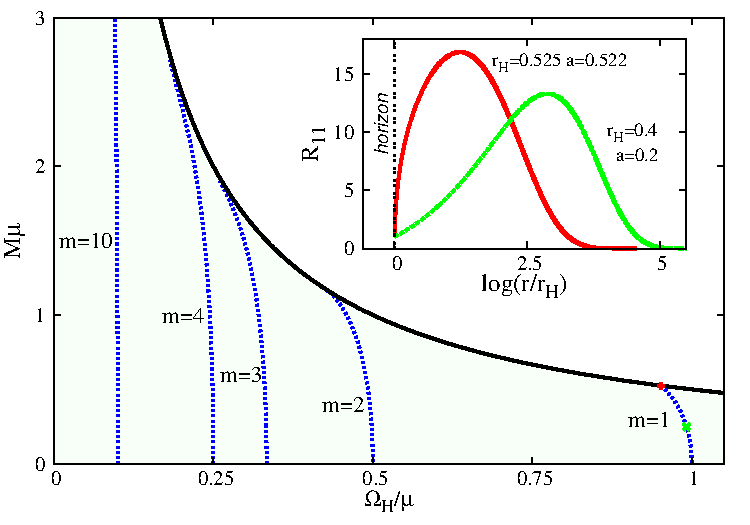
\includegraphics[height=2.78in]{Figs/unstable-OmegaH-M-clouds.pdf}
  \end{center}
  \caption{(Large plot) Mass vs. angular velocity diagram for Kerr black holes. Extremal black holes exist along the black solid line and other Kerr black holes below that line. A few existence lines for scalar clouds are plotted for $n=0$ and for different values of $l=m$ (blue dotted lines). (Inset) Two radial profiles of two particular clouds with $m=1=l$. The clouds are non-zero at the horizon, reach a maximum value at some radial distance and, asymptotically, decrease to zero exponentially. From Ref.~\cite{Herdeiro:2014goa}.}
  \label{fig:clouds}
\end{figure}

Thus, the existence of superradiance admits the existence of bound state solutions (clouds) which are zero modes of this instability.
In the next section we will describe how the backreaction of these clouds on the geometry leads to new black holes with scalar hair.

\section{A new type of hairy black holes}
\label{sec:HBHs}
The scalar clouds described in the previous section suggest that \textit{asymptotically flat rotating black holes with complex scalar hair} could exist.
Such solutions were indeed found in~\cite{Herdeiro:2014goa}, corresponding to a $5$-parameter family of solutions of the Einstein-(massive)-Klein-Gordon theory as described by \eqref{Introaction}.
Three of the parameters are continuous: the ADM mass, $M$, the ADM angular momentum, $J$, and a Noether charge, $Q$.
The last one is obtained by integrating the time component of the scalar field $4$-current on a spacelike slice and may be regarded as measuring the amount of scalar hair outside the horizon.
It is convenient to introduce a normalized Noether charge $q\equiv \frac{Q}{2J}$; then, $q$ is a compact parameter in the full space of solutions: $q\in\left[0,1\right]$.
The value $q=0$ corresponds to Kerr black holes, showing that these hairy black holes are continuously connected to the standard Kerr family, while for $q=1$ rotating boson stars are recovered, which obey $Q=2J$.
The solutions in~\cite{Herdeiro:2014goa} were dubbed \textit{Kerr black holes with scalar hair}.
The two remaining parameters of the solutions found in~\cite{Herdeiro:2014goa} are discrete and have already been described for boson stars: the azimuthal harmonic index $m\in \mathbb{Z}^\pm$ and the node number $n\in \mathbb{N}_0$. 

The hairy black hole solutions were found numerically using a metric ansatz of the form
\begin{align}
  ds^2 &= e^{2F_1}\left( \frac{dr^2}{N} + r^2d\theta^2 \right) + e^{2F_2}r^2\sin^2\theta \left( d\varphi - Wdt \right)^2 - e^{F_0}Ndt^2,
  \label{eqn:HBH-ansatz}
\end{align}
with $N\equiv 1-r_H/r$, and where $F_0,~F_1,~F_2,~W$ are functions of $r$ and $\theta$ only.
$r_H$ is the position of the event horizon of the black hole in this coordinate system.
We remark these are \textit{not} Boyer-Lindquist coordinates in the Kerr limit. 
This metric, or slight variations of it, will be used for all solutions in this thesis.

In~\cite{Herdeiro:2014goa} the parameter and phase space for the solutions with $n=0$, $m=1$ were discussed in detail -- see Fig. \ref{fig:HBH-parameter-space}.
Here are some other relevant features of these solutions.
There is a region of overlap of hairy and Kerr black holes with the same $M,J$ and in that sense there is non-uniqueness.
However, this degeneracy is raised by the introduction of $q$, i.e. no two solutions share the same set of $M,J,q$.
Some of these hairy black solutions violate the Kerr bound: $J\le M^2$.
This is not surprising since this is known to occur for rotating boson stars~\cite{Ryan:1996nk}, and hairy black holes are continuously connected to these stars.
It is indeed a generic feature that hairy black holes are more \textit{star-like} than Kerr black holes, i.e. they are not as tightly constrained in their physical properties as Kerr black holes.
This observation also has implications for possible astrophysical phenomenology of these hairy black holes.
It was observed in~\cite{Herdeiro:2014goa} that both the quadrupole moment and the angular frequency at the innermost stable circular orbit (ISCO) can differ significantly for hairy black holes, as compared to the standard Kerr values.
Finally, hairy black holes have a richer structure of ergo-regions than Kerr, with the occurrence of \textit{ergo-Saturns}, besides ergo-spheres, in a region of parameter space~\cite{Herdeiro:2014jaa}.

\begin{figure}[H]
  \begin{center}
  \includegraphics[height=2.78in]{Figs/BH-w-M.pdf}
 %   \includegraphics[width=\textwidth]{BH-w-M.pdf}
  \end{center}
  \caption{(Large plot) Domain of existence of hairy black holes for $n=0$, $m=1$ in $M$-$w$ space (shaded blue region). The black solid curve corresponds to extremal Kerr black holes, which obey $M={1}/(2\Omega_H)$; Kerr black holes exist below it. For $q=0$, the domain of existence connects to Kerr solutions (dotted blue line). For $q=1$, $r_H$ vanishes and hairy black holes reduce to boson stars (red solid line). The final line that delimits the domain of existence of the hairy black holes corresponds to extremal hairy black holes (dashed green line), i.e. with zero temperature. (Inset) Boson star curves for $m=1,2$. The units in the axes are normalized to the scalar field mass $\mu$. Adapted from Ref.~\cite{Herdeiro:2014goa}.}
  \label{fig:HBH-parameter-space}
\end{figure}

A few observations of these solutions are in order.
As for boson stars, the $t,\varphi$ dependence of the scalar field appears as a phase factor implying that the stress-energy tensor is independent of both these variables which is required for the spacetime to be stationary and axi-symmetric.
The stress-energy tensor will however depend on both $m$ and $w$ and so will the geometry.
Just as for boson stars, there is a single Killing vector field which leaves the whole system invariant given by Eq. \eqref{kvf},
which coincides with the horizon null generator due to Eq. \eqref{super_cond}.
Thus the preservation of the scalar field by this Killing field is reinterpreted as the absence of flux of the scalar field into the black hole.

These solutions also clarify the intriguing aspect discussed at the end of Sec. \ref{sec:bs}.
One can indeed add a black hole at the center of a boson star -- as for other gravitating solitons -- but rotation is mandatory for both the boson star and the black hole.
And this requirement can be understood from the black hole side: only rotating black holes have superradiant instabilities and can thus support scalar clouds. 

In Chapter \ref{ch:Q} we will start with a study of so-called $Q$-clouds which arise from the test field analysis of the Klein-Gordon equation with self-interactions on a Kerr background.
They are generalizations of flat space $Q$-balls to curved spacetimes.
In Chapters \ref{ch:SI}, \ref{ch:proca} and \ref{ch:KN}, we will present generalizations of the hairy black holes discussed above.
Namely, in Chapter \ref{ch:SI}, we will consider two types of self-interactions of the scalar field and show that hairy black hole solutions can also be found there.
In Chapter \ref{ch:proca}, we will consider a Proca field instead of a scalar field.
Finally in Chapter \ref{ch:KN}, we will study electrically charged black holes surrounded by either electrically neutral or charged scalar hair.

In Appendix \ref{appendixb} we give the equations of motion for the model discussed in Chapter \ref{ch:proca} as an illustrative example and show the explicit form of the metric functions for stationary Proca clouds.
In Appendix \ref{BCs} we discuss briefly the boundary conditions and calculation of physical quantities of the Kerr black holes with scalar hair.
This serves as an example as both the boundary conditions and physical quantities are obtained by similar means for all models.
The differences for each model will be discussed in the respective chapters.
For Chapter \ref{ch:SI}, the boundary conditions and physical conditions are identical while for Chapter \ref{ch:KN} there are slight modifications which are discussed in Section \ref{KNBCs}.
In Chapter \ref{ch:proca}, the model is different enough to warrant a longer discussion on both the boundary conditions and physical quantities though much of Appendix \ref{BCs} still applies there.

All numerical solutions in this thesis were obtained with the FIDISOL/CADSOL elliptical solvers\cite{schoen}.
\chapter{$Q$-clouds}
\label{ch:Q}

\epigraph{``\emph{
Ask veit eg standa, \\
heitir Yggdrasill, \\
hár baðmur, ausinn \\
hvíta auri; \\
þaðan koma döggvar \\
þær er í dala falla, \\
stendur æ yfir grænn \\
Urðarbrunni. 
} 
''}{19th verse of Völuspá}
%%%%%%%%%%%%%%%%%%%%%%%%%%%%%%%%%%%%%%%%%%%%%%%%%%%%%%%%%%%%%%%%%%%%%%%%%%%%%%%
\section{Introduction}

$Q$-balls are complex scalar field solitons, obtained with a non-renormalizable self-interaction, arising in some effective field theories. 
These non-topological solitons circumvent the standard Derrick-type argument~\cite{Derrick:1964ww} by virtue of having a
time-dependent phase for the scalar field.
The global phase-invariance of the scalar field theory leads to a conserved Noether
charge $Q$, corresponding to particle number.
Such configurations have a rich structure and
have a number of
of physically interesting applications;
for example, they appear in supersymmetric generalizations of the standard model \cite{Kusenko:1997zq}, 
and have been suggested to generate baryon number or to be dark matter candidates~\cite{Kusenko:1997si}.

\bigskip

Here, we report that $Q$-balls can become $Q$-clouds, when replacing the near (Minkowski) origin region with a black hole horizon\footnote{
Boson shells harbouring black holes have been studied in \cite{Kleihaus:2010ep}.
However, these solutions require a V-shaped scalar potential which
is not of the form (\ref{QU}).}.
This fits into a general pattern observed in soliton physics~\cite{Bizon:1994dh,Volkov:1998cc,Herdeiro:2014ima}; for the case discussed herein, however, the black hole \textit{must rotate}, by virtue of condition (\ref{super_cond}), and the scalar field's frequency is closely related to the rotation of the black hole.
The relation between the scalar field's parameters and the horizon angular velocity can actually be seen as a \textit {rotation synchronization condition}.
%
%
%%%%%%%%%%%%%%%%%%%%%%%%%%%%%%%%%%%%%%%%%%%%%%%%%%%%%%%%%%%%%%%%%%
\section{The model}
%%%%%%%%%%%%%%%%%%%%%%%%%%%%%%%%%%%%%%%%%%%%%%%%%%%%%%%%%%%%%%%%%%



We consider the action for a complex scalar field with a self-interaction potential $U(\left| \Phi \right|)$:
\begin{equation}
\label{Qaction}
S=-\int d^4x\sqrt{-g} \left[ 
   \frac{1}{2} g^{ab}\left( \Phi_{, \, a}^* \Phi_{, \, b} + \Phi _
{, \, b}^* \Phi _{, \, a} \right) + U( \left| \Phi \right|) 
 \right] 
\ . 
\end{equation}
A usual choice for the potential in the $Q$-ball literature is 
\begin{equation}
U(|\Phi|) =  \mu^2 |\Phi|^2-\lambda |\Phi|^4 +\beta |\Phi|^6,
\label{QU} 
\end{equation}
with $\mu$ being the boson mass and $\lambda,\beta>0$.
This potential is chosen such that non-topological soliton solutions
exist in a flat spacetime background, see $e.g.$ the discussion in \cite{Volkov:2002aj}.

Variation of Eq. \eqref{Qaction} with respect to the scalar field
leads to the non-linear Klein-Gordon equation,
\begin{equation}
\label{KG}
 \Box\Phi= \frac{\partial U}{\partial\left|\Phi\right|^2}\Phi \ ,
\end{equation}
where $\Box$ represents the covariant d'Alembert operator.
%
%
The stress-energy tensor $T_{ab}$ of the scalar field is
\begin{eqnarray}
T_{ab} 
=  \Phi_{, \, a}^*\Phi_{, \, b}
+\Phi_{, \, b}^*\Phi_{, \, a} -g_{ab} \left[ \frac{g^{cd} }{2} 
\left( \Phi_{, \, c}^*\Phi_{, \, d}+
\Phi_{, \, \beta}^*\Phi_{, \, \alpha} \right)+U(|\Phi|)\right]
 \ .
\label{tmunu} 
\end{eqnarray}

For the background metric,
we consider a general 
ansatz with two Killing vectors   $\xi=\partial_t$ and $\eta=\partial_\varphi$ (with $t$ and $\varphi$
the time and azimuthal coordinates, respectively),
which in an appropriate coordinate system
can be written as
\begin{eqnarray}
\label{metric-ansatz}
ds^2= g_{rr}dr^2+g_{\theta \theta} d\theta^2 +g_{\varphi\varphi}d\varphi^2+2 g_{\varphi t}d\varphi dt +g_{tt} dt^2 \ .
\end{eqnarray}
$g_{\mu\nu}$ 
are functions of the spherical coordinates $r$ and $\theta$ only. We assume asymptotic flatnes and thus, as $r\to \infty$, $g_{rr} \to 1$,
$g_{\theta \theta} \to r^2$,
$g_{\varphi\varphi} \to r^2\sin^2 \theta$,
$g_{\varphi t} \to 0$
and
$g_{tt} \to -1$.
We also assume the existence of an event horizon, located
at a constant value of $r=r_H$.
This 
is a Killing horizon of the Killing vector field
$\chi=\xi+\Omega_H \eta$,
where $\Omega_H$ is computed as
\begin{eqnarray}
\label{OmegaH}
\Omega_H=-\frac{\xi^2}{\xi \cdot \eta}\bigg |_{r_H}=-\frac{g_{tt}}{g_{t\varphi}}\bigg |_{r_H}.
\end{eqnarray}

The scalar field ansatz is of the form of Eq. \eqref{eqn:field-ansatz}, 
 where $\phi$ is a real function, $w>0$ is the frequency and $m=\pm 1,\pm 2$\dots
is the azimuthal harmonic index. 
As was discussed in the introduction, the $(t, \varphi)$-dependences of $\Phi$ occur as phase factors only.
This implies that $T_{\mu\nu}$ is $(t, \varphi)$-independent, which is required for
a configuration to be stationary and axisymmetric.
The energy-momentum tensor, however,  will 
 depend on both $m$ and $w$.

With the scalar field and metric ansatz given by Eqs. \eqref{eqn:field-ansatz} and (\ref{metric-ansatz}), 
the Klein-Gordon equation Eq. \eqref{KG}
reduces to
\begin{eqnarray}
\label{KG1}
\frac{1}{\sqrt{-g}}\frac{\partial}{\partial r}\left(g^{rr}\sqrt{-g}\frac{\partial \phi}{\partial r} \right)+
\frac{1}{\sqrt{-g}}\frac{\partial}{\partial \theta} \left(g^{\theta \theta}\sqrt{-g}\frac{\partial \phi}{\partial \theta} \right)
\nonumber\\
-\left(
m^2 g^{\varphi \varphi}-2g^{\varphi t} +w^2 g^{tt} 
\right)\phi
=(\mu^2-2 \lambda \phi^2+3\beta \phi^4)\phi.~{~}
\end{eqnarray}
We are interested in 
localized, particle-like solutions of this equation,
 with a finite scalar amplitude $\phi$ and a regular energy density distribution.
These axially symmetric configurations carry a nonzero 
  mass-energy and angular momentum,  which are defined as
\begin{eqnarray}
\label{scalar-charges}
E=-2\pi \int_{r_H}^\infty dr \int_0^\pi d\theta \sqrt{-g}T_t^t\ , \qquad 
J= 2\pi \int_{r_H}^\infty dr \int_0^\pi d\theta \sqrt{-g}T_\varphi^t \ .
 \end{eqnarray}
%
Moreover, a conserved charge $Q$ exists, associated with the complex scalar field $\Phi$, since the Lagrange density is invariant under the global phase transformation
$\Phi \to \Phi e^{i\alpha}$, 
 leading to the conserved current
 \begin{eqnarray}
\label{scalar-current}
j^{a}=-i\left[\Phi^* \partial^a\Phi+\Phi \partial^a\Phi^*\right]\ , \qquad \nabla_aj^{a}=0 \ .
 \end{eqnarray}
The corresponding conserved charge $Q$ is the integral of $j^t$ on spacelike slices.
One can easily see that in the absence of backreaction the following relation holds:
 \begin{eqnarray}
\label{rel1}
J=m Q\ ,
\end{eqnarray}
such that  angular momentum  is quantized.
Moreover,
in view of this relation, the spinning solutions
can be thought of as corresponding to minima of energy with fixed angular
momentum.
 
 
In our approach, $Q$-clouds are found by solving the Klein-Gordon equation Eq. \eqref{KG1}
with suitable boundary conditions.  
Then the energy and angular momentum are computed
from the numerical output.
The boundary conditions result from the study of the solutions
on the boundary of the integration domain. 
The behavior of the scalar field as $r\to \infty$ must agree
with linear analysis: $\phi=f(\theta)  {e^{-\sqrt{\mu^2-w^2}r}}/{r}+\dots$;
thus $\phi|_{r=\infty}$=0, while the existence of a bound state requires $w <\mu $.
Axial symmetry and
regularity impose that the scalar field vanishes on the symmetry axis ($\theta=0,\pi$).
At the horizon, we suppose the existence of a power series expansion of the scalar field,
of the form
\begin{eqnarray}
\label{scalar-horizon}
\phi(r,\theta)=\phi_{0}( \theta)+\phi_{1}( \theta)(r-r_H)+\phi_{2}( \theta)(r-r_H)^2+\dots,
\end{eqnarray}
with finite coefficients $\phi_{k}$.
%
It turns out that, if one assumes $\phi_{0}\neq 0$, such an expansion holds if and only if condition \eqref{super_cond} holds. 
Thus, the synchronization condition is required by regularity and not only as a consequence of wanting to obtain clouds.
After substituting the expansion given by Eq. \eqref{scalar-horizon} into the Klein-Gordon equation, one obtains an involved condition between the coefficients
$\phi_{0}$, $\phi_{1}$ and $\phi_{2}$ 
which should be satisfied at $r=r_H$.
The explicit form of this condition depends on the coordinate system one chooses to work with,
and shall be discussed below.

 

%%%%%%%%%%%%%%%%%%%%%%%%%%%%%%%%%%%%%%%%%%%%%%%%%%%%%%%%%%%%%%%%%%
\section{The solutions}
%%%%%%%%%%%%%%%%%%%%%%%%%%%%%%%%%%%%%%%%%%%%%%%%%%%%%%%%%%%%%%%%%%

 
Similarly to previous works 
\cite{Volkov:2002aj,Kleihaus:2005me}, 
the  numerical solutions reported here have been found for 
the following parameters in 
the potential
defined by Eq. \eqref{QU}:
%
\begin{equation}
\lambda = 2,~~\beta=1,~~\mu^2=1.1~.
\label{param}
\end{equation} 
But solutions with other choices of $\lambda,\beta$
have also been considered.
%
In particular, preliminary results indicate that the constraints
on the potential $U$  required
for the existence of flat space $Q$-balls~\cite{Coleman:1985ki}, 
also hold for the black hole background. 
%
Let us also remark that,
for given $(\mu,w,m)$,
solutions with other values of $\lambda$, $\beta$
can be generated by using the scaling symmetry
\begin{equation}
\phi^{(\lambda_2,\beta_2)}=\sqrt{\frac{\lambda_1}{\lambda_2}}\phi^{(\lambda_1,\beta_1)},~~
E^{(\lambda_2,\beta_2)}=\frac{\lambda_1}{\lambda_2}E^{(\lambda_1,\beta_1)},~~Q^{(\lambda_2,\beta_2)}=\frac{\lambda_1}{\lambda_2}Q^{(\lambda_1,\beta_1)},~~
{\rm with}~~\beta_2=\frac{\lambda_2^2}{\lambda_1}.
\label{symm}
\end{equation} 

All quantities and variables of interest are expressed in natural units set by the scalar field mass $\mu$.

The $Q$-clouds discussed here are invariant under a reflection along  
the equatorial plane; these are commonly referred to, in this context, as \textit{even parity solutions}. Odd parity
solutions, on the other hand, should also exist, and their $Q$-ball limit has been considered in 
\cite{Volkov:2002aj,Kleihaus:2007vk}.

Finally, here we focus on a Kerr black hole background, but similar solutions are likely to exist on any spinning black hole.

%%%%%%%%%%%%%%%%%%%%%%%%%%%%%%%%%%%%%%%%%%%%%%%%%%%%%%%%%%%%%%%%%%
\subsection{Limiting known cases: flat space $Q$-balls and Kerr linear clouds}
%%%%%%%%%%%%%%%%%%%%%%%%%%%%%%%%%%%%%%%%%%%%%%%%%%%%%%%%%%%%%%%%%% 



$Q$-clouds have two known limiting cases: (i) flat space $Q$-balls and (ii) Kerr linear clouds. We shall now briefly review some relevant properties of both these cases which are of interest to understand $Q$-clouds. 

\bigskip


Spinning $Q$-balls have been constructed  in 
\cite{Volkov:2002aj,Kleihaus:2005me};
a review of their properties can be found in \cite{Radu:2008pp}.
%
One imposes that the scalar field
vanishes at the origin, in a spherical coordinate system,  $\phi|_{r=0}=0$, which is implied by demanding regularity of the energy density.
Treating $w,m$ and the parameters in the potential $U$
as input variables, $Q$-balls 
exist only in a certain frequency range, 
$w_{min} < w < w_{max}=\mu$.
An estimate for $w_{min}$
is given by the condition 
\cite{Volkov:2002aj,Kleihaus:2005me}
\begin{eqnarray}
 w_{min}^2\sim  {\rm min} [U(\phi)/\phi^2]=\mu^2-\frac{\lambda^2}{4\beta}<w^2,
\end{eqnarray}
even though this limit could not be reached for spinning solutions.
%
At a critical value of the frequency in the interval $]w_{min}, w_{max}[$, 
both the $Q$-balls' mass-energy and angular momentum attain their minimum value,
from where they monotonically increase towards both limiting values
of the frequency.
%
Thus, considering the $Q$-balls' mass as a function of their Noether charge $Q$,
there are two branches of solutions, merging and ending
at the minimal charge and mass. 
$Q$-balls are stable along (most of) the lower frequency branch~\cite{Radu:2008pp}.
%
For a given frequency, the spatial distribution of the amplitude of the field, i.e. $\phi(r,\theta)$, energy-momentum and charge densities are maximal on the equatorial plane.
The energy is then concentrated in a toroidal region encircling the symmetry-axis.

The limiting behaviour of the spinning $Q$-balls near the boundaries of the allowed frequency interval
is rather intricate, and has not yet been discussed in a systematic way  in the literature. 
It appears that 
both $E$ and $Q$
increase without bound at the limits of the $w$-interval, even though these limits are difficult to investigate.
Additionally, $Q$-balls become there in terms of their spatial distribution there;
as $w\to w_{min}$,
they can be viewed as squashed spheroids, homogeneously filled inside.
For $w\to w_{max}$, the solutions
also become large spheroids, but this time they are hollow, with the maximal energy density
concentrated at the surface and being close to zero everywhere else.  

\bigskip
  
A very different picture has been found in~\cite{Herdeiro:2014goa,Benone:2014ssa}
for the simpler case of a non-self-interacting
scalar field
on a fixed Kerr black hole background.
These linear scalar clouds
satisfy the same boundary conditions as stated above.
However, their study is  simpler, since in this case
the Klein-Gordon equation admits separation of variables. 
%
Then the problem reduces to solving
an ordinary differential equation for 
the radial function $R_{nlm}(r)$.
This has been done in~\cite{Herdeiro:2014goa,Benone:2014ssa} and determines the position of the existence lines for a cloud with quantum numbers $(n,l,m)$. Three examples of these lines are exhibited in Fig. \ref{existencelines}, in a mass ($M$) vs. horizon angular velocity ($\Omega_H$) diagram for Kerr black holes.
%
Analytical estimates for these lines have been found in 
\cite{Hod:2012px,Hod:2013zza}
for the case of a (nearly-)extremal Kerr black hole.


\begin{figure}[h!]
\centering
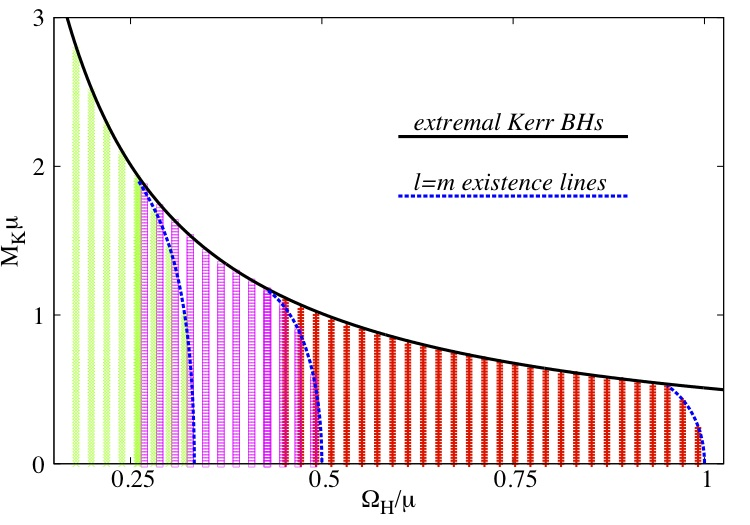
\includegraphics[height=2.8in]{papers/QClouds/Mw.jpeg}
\caption{Existence (blue dotted) lines with $n=0$, $m=l=1,2,3$, from right to left, respectively, for linear clouds on the Kerr background.  Kerr black holes exist below the solid black line, which corresponds to extremal Kerr solutions. For each $m$, $\Omega_H^{extremal}$ is the value of $\Omega_H$ at which the corresponding existence line intersects the curve of extremal black holes. The (vertical sets of) filling points in the diagram correspond to examples of $Q$-cloud solutions with $m=1$ (red/dark grey), $m=2$ (purple/medium grey) and $m=3$ (green/light grey). $Q$-clouds with a given value of $m$ exist between the existence line for linear clouds with $n=0$, $m=l$ and a minimal frequency.} 
\label{existencelines}
\end{figure}

The existence line with $n=0$ and $l=m$ divides the Kerr parameter space in two regions. To the left (right) of the line stand the Kerr backgrounds which are superradiantly stable (unstable) against scalar field perturbations with azimuthal harmonic index $m$.


%%%%%%%%%%%%%%%%%%%%%%%%%%%%%%%%%%%%%%%%%%%%%%%%%%%%%%%%%%%%%%%%%%
\subsection{Non-linear $Q$-clouds on the Kerr black hole background}
%%%%%%%%%%%%%%%%%%%%%%%%%%%%%%%%%%%%%%%%%%%%%%%%%%%%%%%%%%%%%%%%%%

When turning on the scalar field self-interactions in the potential, i.e. giving them a small but non-zero value, the non-linearities prevent a separation of variables.
For given $(w,m)$,
the scalar field $\phi$ is a superposition of
spheroidal harmonics, whose amplitudes, however, differ from $R_{nlm}(r)$.
Then following \cite{Volkov:2002aj}, one can write
% 
\begin{eqnarray}
\phi(r,\theta)=\sum_{k=0}^\infty f_k(r)S_{m+2k,m} (\theta),
\end{eqnarray}
%
which results in an infinite set of ordinary differential
equations for $f_k(r)$.
In principle, this set can be truncated for some $k_{max}$
and then solved numerically.
In our approach, however, we have chosen to solve
 directly the partial differential equation (\ref{KG1}). But instead of using Boyer-Lindquist coordinates -- 
 which yield a complicated boundary condition at  $r=r_H$,  in terms of the scalar function and its first and second derivatives -- we have used quasi-isotropic coordinates for Kerr (see e.g.~\cite{Cook:2000vr}).  In parallel, a large set of solutions have been computed  by using a radially shifted version of the Boyer-Lindquist coordinate system, for which $r\to r-\frac{a^2}{r_H}$.
%
Both these coordinate systems yield a near horizon expansion for the scalar field, defined in Eq. \eqref{scalar-horizon}, with the $\phi_1$ term absent, thus allowing us to impose a standard Neumann boundary condition there.
                                                                
  
Our central result in this chapter is
that {\it all flat space Q-ball solutions can be generalized to Q-clouds on a Kerr black hole background}.
The black hole parameters, however, are not arbitrary, as implied by condition (\ref{super_cond}).
%
%
The solutions are found by starting with a flat spacetime
configuration with given $(w,m)$ and increasing the size of the black hole
(as given $e.g.$ by the event horizon area)
via the parameter $r_H$.  
We have constructed in a systematic way solutions with $m=1,2,3$. A subset of the solutions for each of these values of $m$ has been plotted in Fig.~\ref{existencelines}.  When varying the horizon size, there are two 
possible behaviours for the solutions with a given $w$: 
\begin{itemize}
\item[(i)]

For $m\Omega_H^{extremal}/\mu\leq w/\mu <1$,  $Q$-clouds start from flat spacetime $Q$-balls (i.e. with zero horizon size)
 and end on the existence line for linear clouds with $n=0$, $l=m$. The value of $\Omega_H^{extremal}$ depends on $m$; for instance,  $\Omega_H^{extremal}\simeq 0.95,0.43,0.26$  for $m=1,2,3$, respectively (see $e.g.$~\cite{Hod:2013zza}). As the existence line is approached,
the amplitude of the scalar field
decreases to zero and 
the linear scalar clouds are recovered.
 
\item[(ii)]
For  $m\Omega_H^{min}\leq w <m\Omega_H^{extremal}$,
any Kerr black hole with $\Omega_H=w/m$ is allowed as a background for a $Q$-cloud solution.
In particular, one finds scalar clouds also on extremal Kerr black holes,
which provide one boundary for the domain of existence. Again, the value of $\Omega_H^{min}$ depends on $m$ and they seem to coincide, in terms of $w_{min}$, with the corresponding value for $Q$-balls.
%

\end{itemize}
%
The bottom line is that $Q$-clouds exist between the $l=m$, $n=0$ existence line for linear clouds and a minimal frequency/horizon angular velocity -- cf. Fig. \ref{existencelines}. A number of configurations with $m=4,5$
have also been found, not presented here;
thus we expect their existence for any $m\geq 1$.

A generic $Q$-cloud solution has nonzero mass and angular momentum,
with a toroidal distribution for the corresponding densities -- Fig. \ref{densities}.
% 
The scalar profile looks rather similar to that known in the flat spacetime limit
(with the region $r<r_H$ removed from it).
Note, however, that similarly to the behaviour observed for linear scalar clouds~\cite{Benone:2014ssa}, 
the scalar field amplitude does not vanish at the horizon,
approaching its maximum on the equatorial plane.
The energy density $-T_t^t$
vanishes on the symmetry axis, except for $m=1$ solutions.


\begin{figure}[h!]
\centering
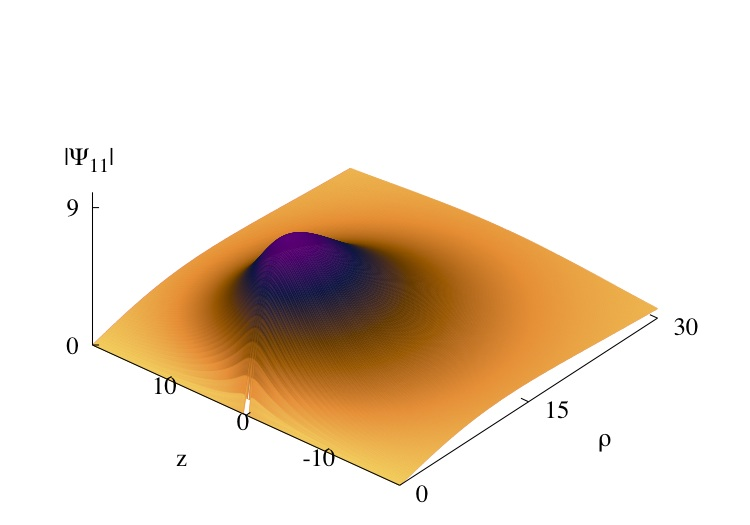
\includegraphics[height=2.2in]{papers/QClouds/Z-3d.jpeg}
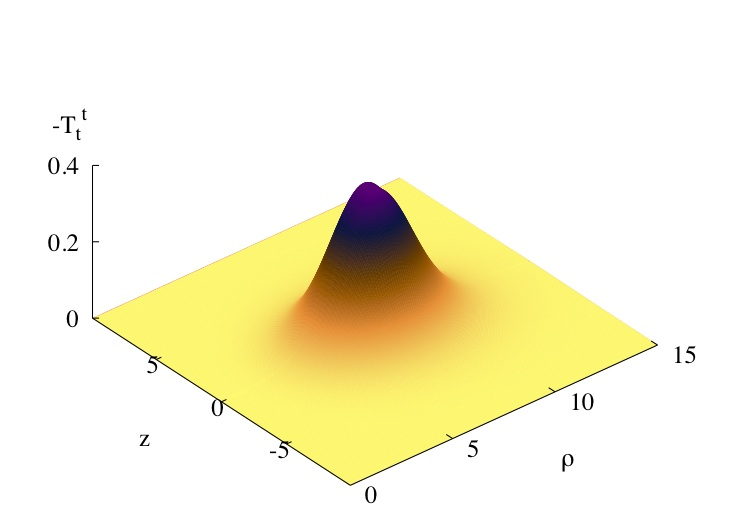
\includegraphics[height=2.2in]{papers/QClouds/E-3d.jpeg}
\caption{The scalar field and the energy density are shown for a typical
 non-linear $Q$-cloud with $m=2$, $w =1$ (in terms of `polar' coordinates $\rho=r\sin \theta$,
 $z=r \cos \theta$).
The Kerr black hole background has an event horizon radius (in quasi-isotropic coordinates) at
 $r_H=0.03$. 
} 
\label{densities}
\end{figure}

In Fig. \ref{energy1}, we plot the energy 
of $Q$-clouds as a function of several parameters of the Kerr black hole background. These results have been obtained for $m=1$, but a similar picture has been found for $m=2,3$. A similar pattern is observed for the angular momenta $J$.

\begin{figure}[h!]
\centering
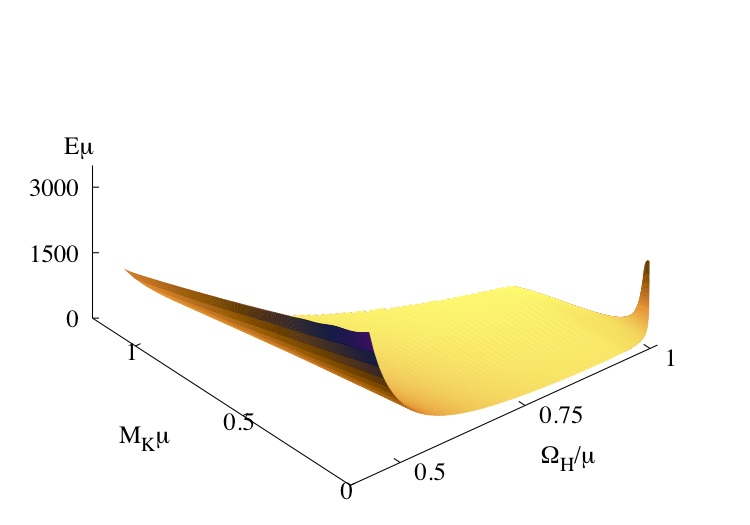
\includegraphics[height=2.15in]{papers/QClouds/EMw-3D.jpeg}
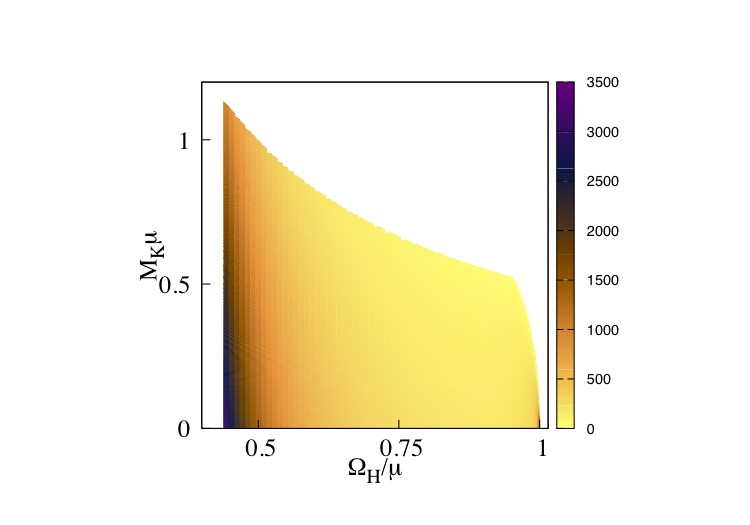
\includegraphics[height=2.15in]{papers/QClouds/EMw-2D.jpeg}
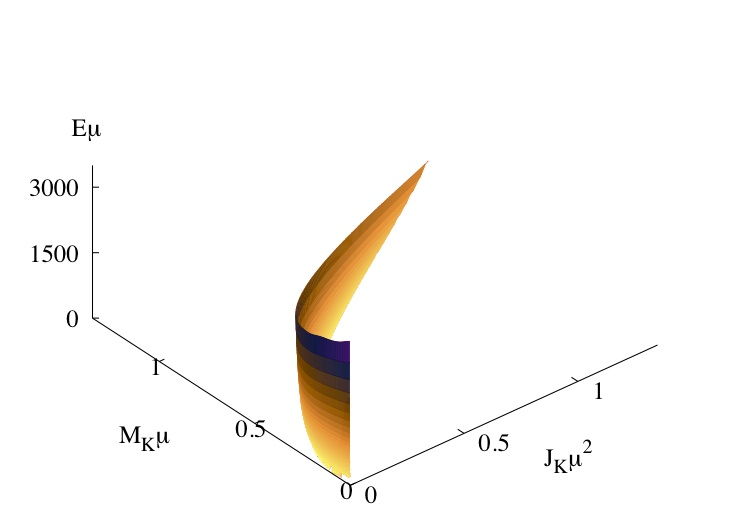
\includegraphics[height=2.15in]{papers/QClouds/EMJ-3D.jpeg}
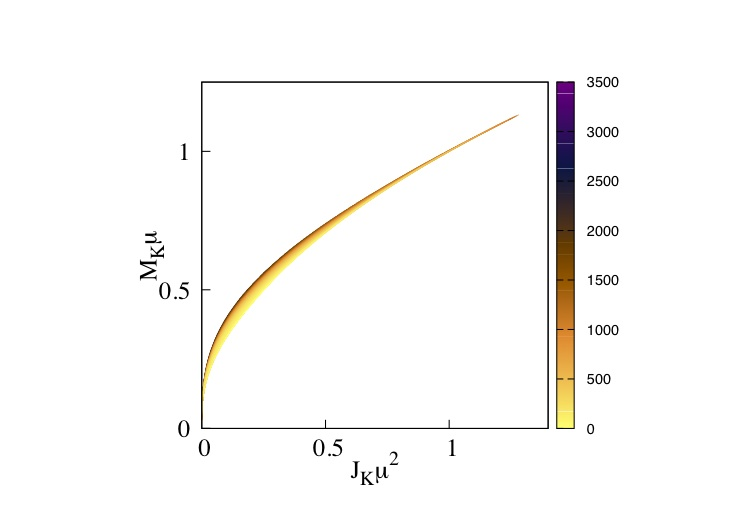
\includegraphics[height=2.15in]{papers/QClouds/EMJ-2D.jpeg}
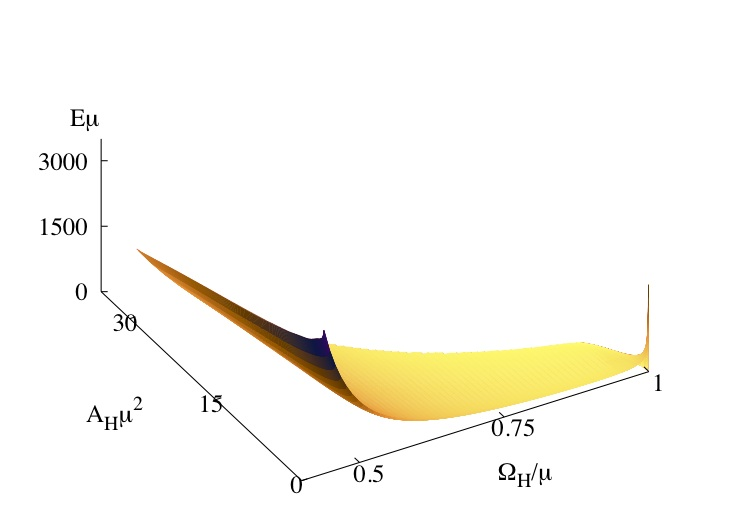
\includegraphics[height=2.15in]{papers/QClouds/EAHw-3D.jpeg}
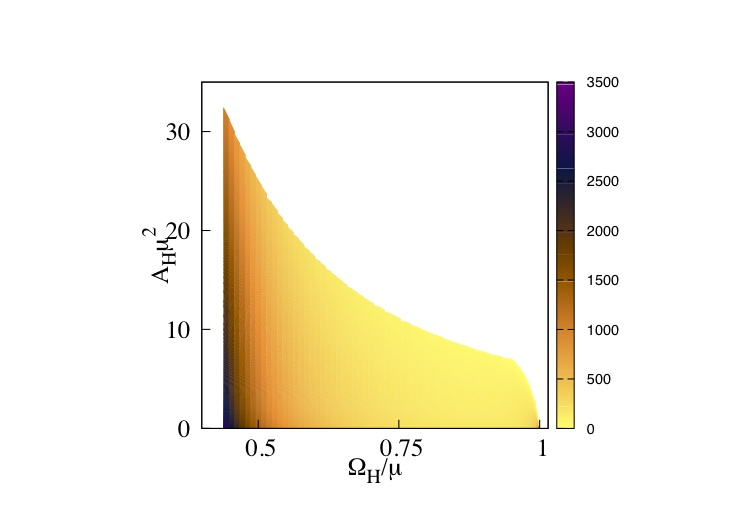
\includegraphics[height=2.15in]{papers/QClouds/EAHw-2D.jpeg}
\caption{$Q$-clouds energy, $E$, as a function three different combinations of parameters for the Kerr background, exhibited in both 3-dimensional (left panel) and 2-dimensional (right panel) plots: (top panel) mass $M_K$ and event horizon velocity $\Omega_H$; (middle panel) $M_K$ and angular momentum $J_K$; (lower panel) event horizon area $A_H$ and  $\Omega_H$.   
} 
\label{energy1}
\end{figure}

Similarly to the flat spacetime case,
  the study of the solutions with $w\to w_{min}$
  is rather difficult, since
 both the energy and angular momentum of the $Q$-clouds 
 take very large values in this limit. 
 At the same time, and in contrast to flat space $Q$-balls, the charges of $Q$-clouds
 remain finite as the maximal frequency is approached. In this case, the black hole background plays the role of a regulator.
 %
 These limiting behaviours are illustrated in Fig. \ref{spectrum}, where we plot the energy spectrum of $m=1$ $Q$-balls,
 $E(w)$,
 for several fixed values of the horizon area $A_H$.
 One can see that $Q$-clouds on a ``small''  Kerr black hole
 approach  for $w_{max}<\mu$,
 a critical configuration with zero global charges; this configuration sits 
 on the corresponding ($n=0,~l=m$)  existence line.
On the other hand, $Q$-clouds on a ``large'' Kerr black hole 
 end at a critical configuration with nonzero mass-energy and angular momentum;
 the corresponding Kerr backgrounds have $T_H=0$. 
 
 \begin{figure}[h!]
\centering
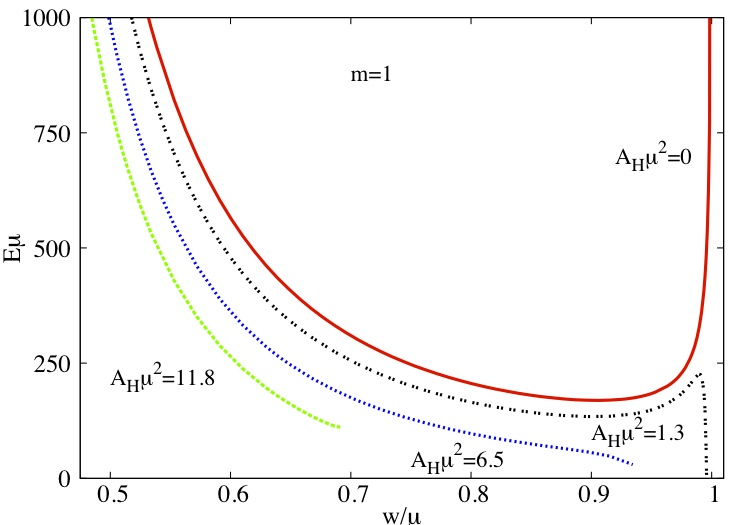
\includegraphics[height=2.8in]{papers/QClouds/Ew-fixed-AH.jpeg}
\caption{The spectrum of $Q$-clouds for several
fixed values of the event horizon area $A_H$.
The solutions with $A_H=0$
are the flat space $Q$-balls.} 
\label{spectrum}
\end{figure}
   
 
 
 %%%%%%%%%%%%%%%%%%%%%%%%%%%%%%%%%%%%%%%%%%%%%%%%%%%%%%%%%%%%%%%%%%%%%%%%%%%%%%%
\section{Discussion} 
%%%%%%%%%%%%%%%%%%%%%%%%%%%%%%%%%%%%%%%%%%%%%%%%%%%%%%%%%%%%%%%%%%%%%%%%%%%%%%%

We have shown that
the well-known flat space $Q$-balls 
possess generalizations to a rotating black hole background -- $Q$-clouds. These bound states are 
in synchronous rotation with the black hole horizon, i.e. they obey condition (\ref{super_cond}).
Remarkably,
the self-interactions allow the existence of non-linear clouds 
in a \textit{2-dimensional} subspace of the full parameter space of Kerr black holes.
%
This subspace is bounded by the flat spacetime $Q$-balls,
the  $n=0,l=m$ existence line of linear clouds~\cite{Benone:2014ssa}
and a critical curve delimited by the minimal frequency of the scalar field,
and extremal Kerr black holes.
 
The backreaction of $Q$-clouds leads to a new family of Kerr black holes with scalar hair in the full Einstein-scalar field system, when this type of self interactions are included. The new solutions have quantitative and qualitative differences, relatively to the Kerr black holes with scalar hair found in~\cite{Herdeiro:2014goa}. We have obtained some examples of these solutions, both for the self interactions studied here and another case.
This will be discussed at the end of Chapter \ref{ch:SI}.

Finally, let us mention that we have found no bound state solutions on the Kerr background for self-interacting scalar fields with the renormalizable potential $U(|\Phi|) =  \mu^2 |\Phi|^2+\lambda |\Phi|^4$.
However, as we will see in the next chapter, hairy black holes with such a potential do exist.
In a similar spirit,  boson stars can exist for this potential~\cite{Colpi:1986ye,Schunck:2003kk},  but they trivialize in the flat space limit, since the potential does not support $Q$-balls. 
\chapter{Kerr black holes with self-interacting scalar hair}
\label{ch:SI}

\epigraph{``\emph{
Það man hún fólkvíg \\
fyrst í heimi, \\
er Gullveigu \\
geirum studdu \\
og í höll Hárs \\
hana brenndu, \\
þrisvar brenndu, \\
þrisvar borna, \\
oft, ósjaldan; \\
þó hún enn lifir. 
} 
''}{21st verse of Völuspá}


%%%%%%%%%%%%%%%%%%%%%%%%%%%%%%%%%%%%%%%%%%%%%%%%%%%%%%%%%%%%%%%%%%%%%%%%%%%%%%%
\section{Introduction}
% %%%%%%%%%%%%%%%%%%%%%%%%%%%%%%%%%%%%%%%%%%%%%%%%%%%%%%%%%%%%%%%%%%%%%%%%%%%%%%%
Boson stars are self-gravitating solitons.
In their simplest guise, they arise as solutions of General Relativity minimally coupled to a massive, free, complex scalar field\cite{Kaup:1968zz,Ruffini:1969qy}.
This simple model presents only two dimensionful parameters (or scales): Newton's constant $G$ (which can be rephrased as the Planck mass $M_{\rm Pl}$) and the scalar field mass $\mu$.
As for fermionic stars, the effective pressure of the scalar field cannot withstand an infinite amount of mass without undergoing gravitational collapse into a black hole (BH).
Intuitively, the smaller the scalar field mass, the larger the maximal mass of the star can be, since the scalar particle's Compton wavelength is larger and hence these particles are less confined. 
Actual calculations show this maximal mass to be of the order of the scalar field's Compton wavelength
\begin{equation}
 M_{\rm ADM}^{\rm max}\simeq \alpha_{\rm BS} \frac{M_{\rm Pl}^2}{\mu}\simeq \alpha_{\rm BS} \, 10^{-19}M_\odot\left(\frac{\rm GeV}{\mu}\right)\ , 
\label{mini}
\end{equation}
where $M_{\odot}$ is the Sun's mass and $\alpha_{\rm BS}$ is found, numerically, to be of order of unity.
Observe that the maximal mass is small, by astrophysics standards, for scalar field masses within the range of the standard model of particle physics.
As such, in the literature these boson stars are known as \textit{mini-}boson stars\cite{Schunck:2003kk}. 

The scalar field profile of such a boson star generally has a number of nodes, or roots, $n\in \mathbb{N}_0$. The $n=0$ case corresponds to fundamental states whereas $n>0$ are excited states. We shall focus on the former, since they are the most stable configurations.
Furthermore, we will study solutions with $m=1$, where $m$ is the azimuthal harmonic index.
It has been shown that the maximal mass increases with increasing $m$.\cite{Liebling:2012fv,Yoshida:1997qf,Grandclement:2014msa}
This increase, however, requires  unreasonably high values of $m$, for the mass to be of order $M_{\odot}$, when $\mu$ is in the mass range of standard model particles. Ultra-light scalar fields
, on the other hand, can yield astrophysical masses even for small $m$. 

A different approach to increase the maximal mass of boson stars is to include self-interactions for the scalar field.
It was found by Colpi et al.\cite{Colpi:1986ye} that for spherically symmetric \textit{quartic}-boson stars the maximal mass can be considerably higher:

\begin{equation}
 M_{\rm ADM}^{\rm max}\simeq 
0.062  \sqrt{\lambda}\frac{M_{\rm Pl}^3}{\mu^2}\simeq 0.062  \sqrt{\lambda}M_\odot \left(\frac{\rm GeV}{\mu}\right)^2\ .
\label{csw}
\end{equation}
Here, $\lambda>0$ is the self-interaction coupling where the self-interaction potential is given by $V(|\Psi|)=\lambda|\Psi|^4$.
It is therefore clear that by choosing a suitable $\lambda$, an astrophysically relevant mass can be obtained for boson stars, even for typical standard model particles.

For rotating boson stars, similar results were found by Ryan~\cite{Ryan:1996nk} for the large self-interaction limit, while later work considered a single value of the coupling and higher $m$ solutions~\cite{Grandclement:2014msa,Kleihaus:2015iea}.
In this chapter, we will present a more systematic study of rotating quartic-boson stars in terms of $\lambda$.
In particular, the analogue of Eq.~\eqref{csw} was obtained for $m=1$ solutions ($cf.$ Fig.~2 in Ref.~\cite{Herdeiro:2015tia}):
%
\begin{equation}
M_{\rm ADM}^{\rm max}\simeq 
0.057  \sqrt{\lambda}\frac{M_{\rm Pl}^3}{\mu^2}\simeq 0.057  \sqrt{\lambda}M_\odot \left(\frac{\rm GeV}{\mu}\right)^2\ .
\label{quartic_rotating}
\end{equation}

However, our interests do not lie solely in the area of boson stars.
We want to consider black hole solutions with self-interacting scalar hair.
Therefore one may ask, what the maximal \textit{horizon} mass, rather than ADM mass, for KBHsSH is and whether this mass is affected by self-interactions.
The former is well defined in terms of a Komar integral.
A first analysis of horizon mass and angular momentum for KBHsSH was presented in~\cite{Herdeiro:2015moa} where it was pointed out that the Kerr bound can be violated in terms of horizon quantities.

We will start this chapter by discussing the model in question, though there are very few differences between it and the model discussed in Chapter \ref{ch:intro}.
We will then study quartic-boson stars, i.e. boson stars with a $\phi^4$ self-interaction coupling.
In the following two sections, we will look at KBHsSH with quartic self-interactions.
Namely, first their asymptotic quantities and then their horizon quantities.
Finally, we will discuss some of the consequences of our results and show that they might be a general phenomena to all self-interaction potentials.

% The goal of this chapter is to make a different observation: the maximum horizon mass $M^{\rm max}_H$ for KBHsSH is attained at a particular configuration we dub the \textit{Hod point}, corresponding to the extremal (vacuum) Kerr BH obtained in the vanishing hair limit, and precisely one of the points studied in~\cite{Hod:2012px}.
% For KBHsSH this maximal mass obeys the same form as \eqref{mini},
% \begin{equation}
%   M_{\rm H}^{\rm max}\simeq \alpha_{\rm Hod} \frac{M_{\rm Pl}^2}{\mu}\simeq \alpha_{\rm Hod} \, 10^{-19}M_\odot\left(\frac{\rm GeV}{\mu}\right)\ , 
% \label{hodpoint}
% \end{equation}
%  but with the constant $\alpha_{\rm Hod}<\alpha_{\rm BS}$. For instance, for $m=1;2$, $\alpha_{\rm Hod}=0.526; 1.165$. 
 
%%%%%%%%%%%%%%%%%%%%%%%%%%%%%%%%%%%%%%%%%%%%%%%%%%%%%%%%%%%%%%%%%%%%%%%%%%%%%%%
\section{The model}
\label{SIsec_model}
%%%%%%%%%%%%%%%%%%%%%%%%%%%%%%%%%%%%%%%%%%%%%%%%%%%%%%%%%%%%%%%%%%%%%%%%%%%%%%% 
 
We shall consider a massive, complex scalar field, $\Psi$, minimally coupled to Einstein's gravity. The action is:
%
\begin{eqnarray}
  \label{Intaction}
  &&
	\mathcal{S} = \int d^4x \sqrt{-g}\left[\frac{R}{16\pi G}- g^{ab}\Psi^*_{,a}\Psi_{,b} - U(|\Psi|)\right],~~{~~} \ \  
\\
\label{pot}
&&~~~~{\rm with}~~~U(|\Psi|)= \mu^2\left|\Psi\right|^2 + \lambda\left|\Psi\right|^4,
\end{eqnarray}  
where $G$ is Newton's constant, $\mu$ is the scalar field mass and the self-coupling is positive, $ \lambda>0$. 
%
To describe both spinning boson stars and KBHsSH we take the metric and field ansatz defined by Eq. \eqref{eqn:HBH-ansatz} and \eqref{eqn:field-ansatz}.

The Einstein-Klein-Gordon equations obtained from \eqref{Intaction} yield a system of five coupled, non-linear PDEs, together with two constraint equations, found 
by taking $\mu^2\to \mu^2+ \lambda \phi^2$ ($\mu^2\to \mu^2+2\lambda \phi^2$) in the Einstein (Klein-Gordon) equations, as displayed in~\cite{Herdeiro:2015gia}.
The boundary conditions used to solve these
equations are different depending whether one considers boson stars or KBHsSH, but do not depend on $\lambda$, and can be found in Appendix \ref{BCs} for the black hole case.


%%%%%%%%%%%%%%%%%%%%%%%%%%%%%%%%%%%%%%%%%%%%%%%%%%%%%%%%%%%%%%%%%%%%%%%%%%%%%%%
\section{Quartic-Boson Stars}
\label{sec_II}
%%%%%%%%%%%%%%%%%%%%%%%%%%%%%%%%%%%%%%%%%%%%%%%%%%%%%%%%%%%%%%%%%%%%%%%%%%%%%%% 
We start by considering quartic-boson star solutions and their dependence on the coupling $\lambda$. These solutions are  conveniently presented in an ADM mass $vs.$ scalar field frequency diagram, as shown in Fig. \ref{fig:w-vs-M-BSs}. In this type of diagram, for $\lambda=0$, it is well known that the boson star solutions form a spiraling curve (see $e.g.$~\cite{Herdeiro:2015gia}). The solutions start from vacuum ($w=\mu$), at which point they trivialize. As $w$ decreases from this value, their ADM mass increases until reaching a maximum value at $w_{\rm max}\simeq 0.775 \mu$. A minimum frequency is then reached after which the curve backbends towards a second branch. A second backbending and a third branch can be seen in  Fig. 1 of~\cite{Herdeiro:2015gia}.

\begin{figure}[h!]
  \begin{center}
    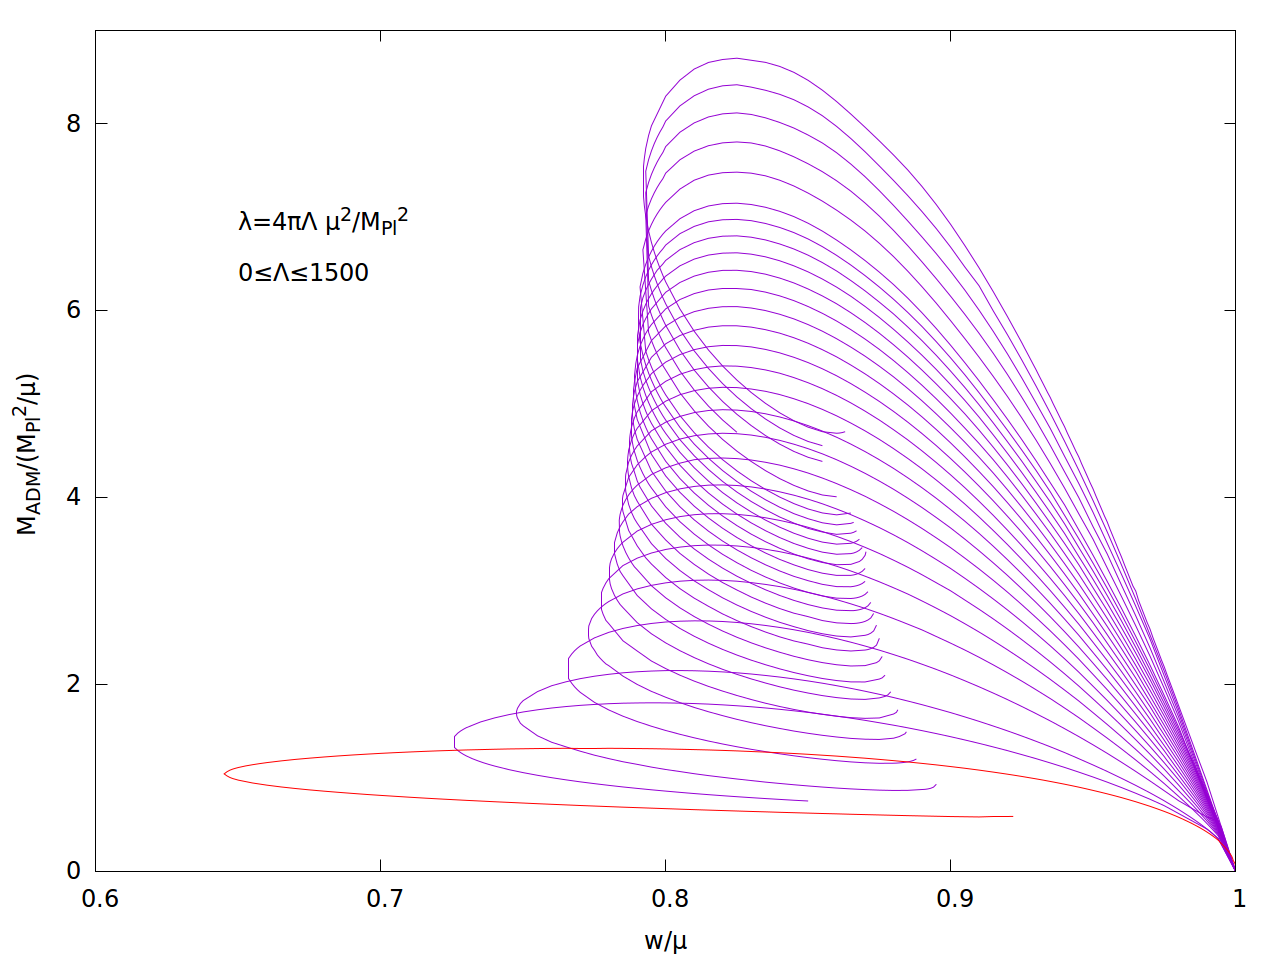
\includegraphics[width=0.7\textwidth]{papers/selfInteractions/w-vs-M-BSs2.png}
  \end{center}
  \caption{ADM mass of $m=1$, nodeless boson stars, as a function of $w$, for various values of $\lambda$ (defined by $\Lambda$, used in numerics): (from bottom to top) $\Lambda=0$ (red curve), $\Lambda=25$, $\Lambda=50-1000$ in steps of $50$, and $\Lambda=1000-1500$ in steps of $100$. Each curve was drawn from, typically, one hundred solution points.}
  \label{fig:w-vs-M-BSs}
\end{figure}



A similar description applies for $\lambda\neq 0$. In Fig. \ref{fig:w-vs-M-BSs} we can see how boson star spiral changes as the quartic coupling parameter $\lambda$ varies from zero -- the mini-boson star case -- to a large value. The typical trend is that the spiral-like behaviour is still kept as $\lambda$ increases, with an increase of the maximal mass. The range of frequencies becomes slightly smaller with increasing coupling. Each curve in Fig. \ref{fig:w-vs-M-BSs} continues after the local minimum of the mass towards a third branch which has been omitted for simplicity, but can be observed in the plots of the next section for a handful of values. Finally, observe that all boson star curves merge at the origin, where they trivialize. 

From the data exhibited in Fig.~\ref{fig:w-vs-M-BSs} one obtains the maximal mass $M_{\rm ADM}^{\rm max}$ $vs.$ $\lambda$ exhibited in Fig.~\ref{max_mass_0}; for large $\lambda$ the data points are well fitted by Eq. \eqref{quartic_rotating}.
%
\begin{figure}[h!]
  \begin{center}
    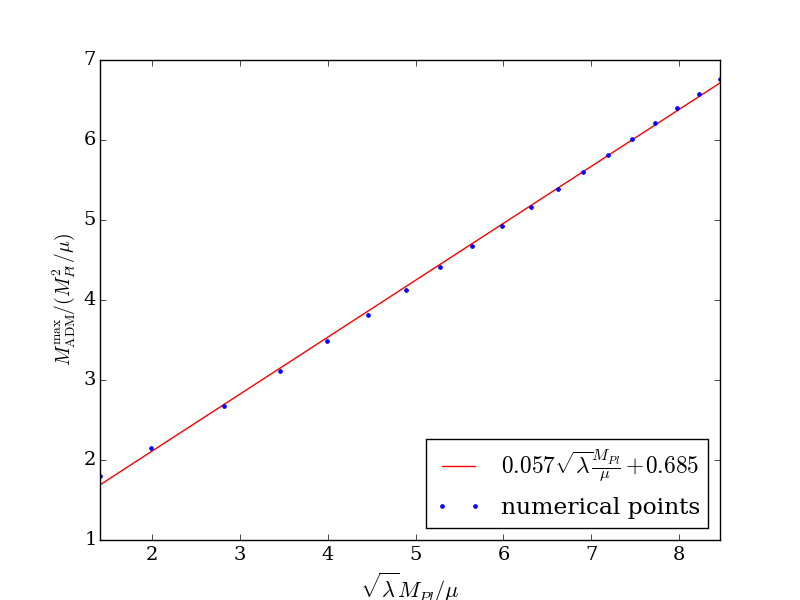
\includegraphics[width=0.7\textwidth]{papers/selfInteractions/max-mass.png}
  \end{center}
  \caption{$M_{\rm ADM}^{\rm max}$ for boson stars $vs.$ the coupling constant $\lambda$, using the data in Fig.~\ref{fig:w-vs-M-BSs}, together with a numerical fit.}
  \label{max_mass_0}
\end{figure}
%






%%%%%%%%%%%%%%%%%%%%%%%%%%%%%%%%%%%%%%%%%%%%%%%%%%%%%%%%%%%%%%%%%%%%%%%%%%%%%%%
\section{Quartic-KBHsSH: ADM quantities}
\label{sec_III}
%%%%%%%%%%%%%%%%%%%%%%%%%%%%%%%%%%%%%%%%%%%%%%%%%%%%%%%%%%%%%%%%%%%%%%%%%%%%%%%
We now turn to KBHsSH and consider first no self-interactions. For nodeless, $m=1$ KBHsSH, their domain of existence, in an ADM mass $vs.$ $w$~\cite{Herdeiro:2014goa,Herdeiro:2015gia} is shown in the left panel of Fig.~\ref{kbhsh1}.  The black solid line represents extremal BHs {with horizon angular velocity}
\begin{eqnarray}
\label{SIcond}
 \Omega_H=\frac{w}{m} \ .
\end{eqnarray} 
We recall this is the synchronization condition which underlies KBHsSH. (Vacuum) Kerr BHs exist in this diagram below this line.
The domain of existence of KBHsSH is bounded by the same curves as discussed in Chapter \ref{ch:intro} and shown in Fig. \ref{fig:HBH-parameter-space}.
% \begin{description}
% \item[i)] the corresponding boson star curve (red solid line), for which we display the first three branches;
% \item[ii)] by a line of extremal ($i.e.$ zero temperature) KBHsSH (green dashed line);
% \item[iii)] and by a line of (vacuum) Kerr BHs (blue dotted line), corresponding to the Kerr solutions that allow the existence of stationary scalar clouds with the appropriate set of quantum numbers~\cite{Herdeiro:2014goa,Benone:2014ssa}.   
% \end{description}
We want to draw attention to the so-called ``Hod point" (grey dot in the figures of this section), which lies at the intersection of boundaries ${\bf ii)}$ and ${\bf iii)}$, corresponding to the extremal (vacuum) Kerr BH obtained in the limit of vanishing scalar field.
Remarkably, at the Hod point, the scalar field possesses a relatively simple closed form~\cite{Hod:2012px}.
% in terms of hypergeometric functions and spheroidal harmonics.


When a quartic self-interaction is included for the scalar field, it was already shown in~\cite{Kleihaus:2015iea} that a similar pattern occurs, for a particular value of the coupling. In the right panel of Fig.~\ref{kbhsh1} we show the domain of existence of KBHsSH for four different values of the coupling $\lambda$, given by $\Lambda=0,100,350,750$. Each domain of existence has been filled in by thousands of numerical points. As can be observed, as the coupling is varied, boundaries  ${\bf i)}$ and ${\bf ii)}$ change, and seem to be delimiting a gradually thinner ribbon in this diagram. Boundary  ${\bf iii)}$, however, is invariant, and so is the Hod point, as the self-interaction of the scalar field become irrelevant in the probe limit. In particular, this analysis confirms that the maximal ADM mass for quartic-KBHsSH is that of the corresponding boson stars, and so it is still given by~\eqref{quartic_rotating}.




\begin{figure}[h!]
  \begin{center}
    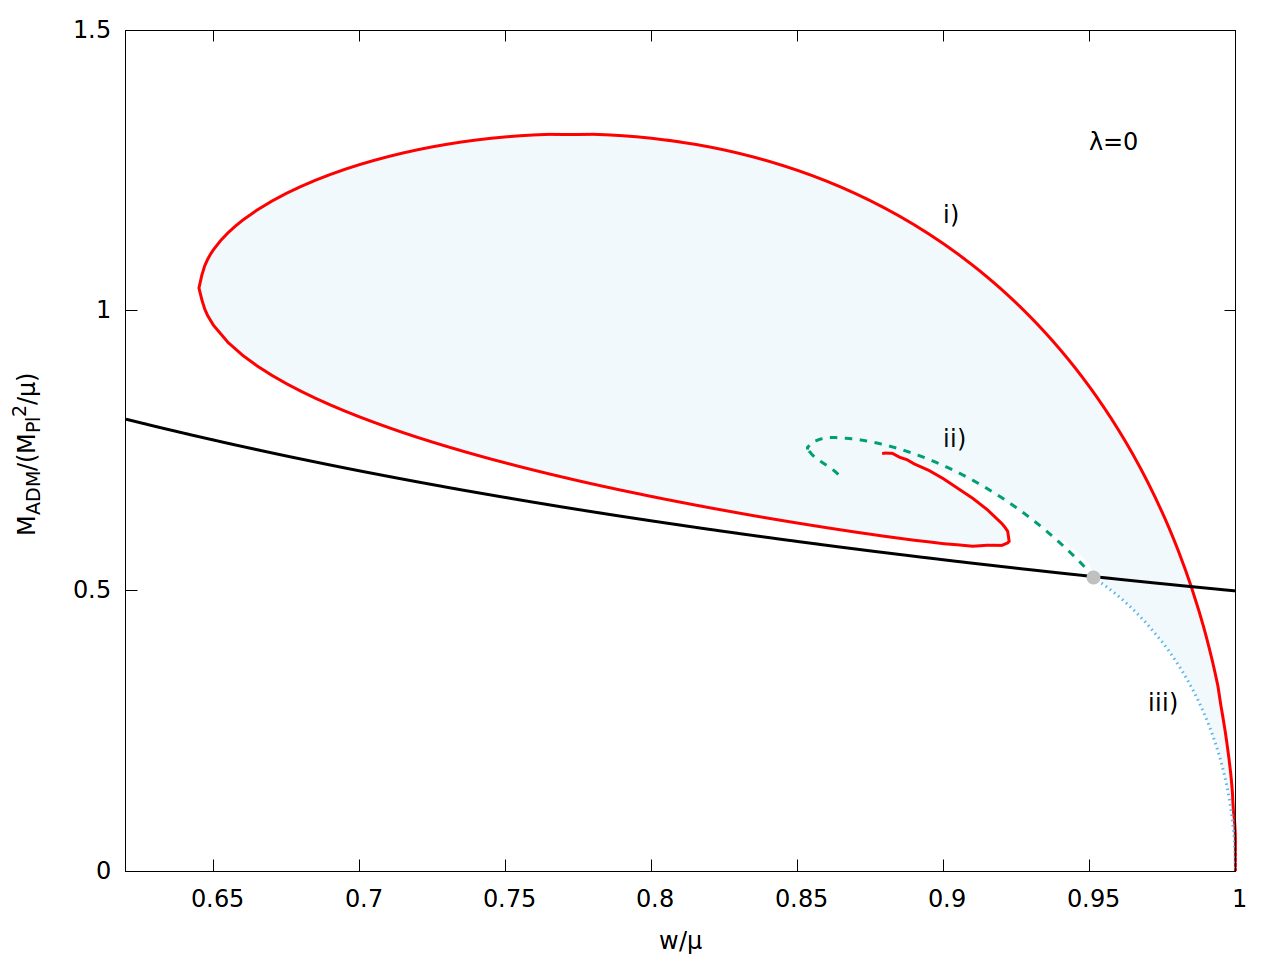
\includegraphics[width=0.48\textwidth]{papers/selfInteractions/w-vs-M-0.png}
    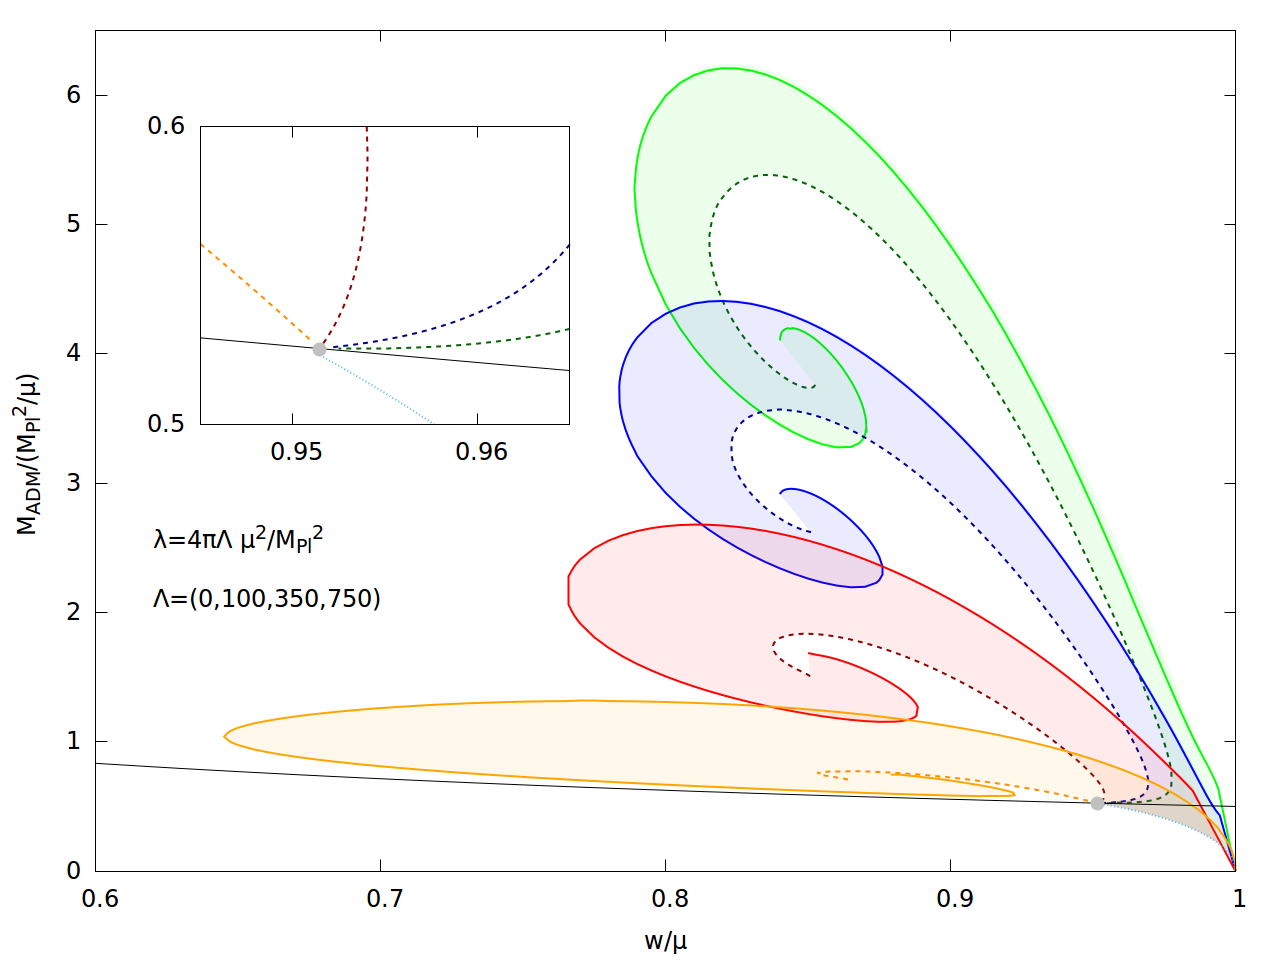
\includegraphics[width=0.48\textwidth]{papers/selfInteractions/BH-w-Mtimes4.png}
      \end{center}
  \caption{(Left) Domain of existence of KBHsSH without self-interactions (blue shaded region).(Right) Domain of existence of KBHsSH for $\Lambda=0,100,350,750$ (shaded regions, from the lowest to the highest, respectively). The inset shows a detail around the Hod point (grey dot).}
  \label{kbhsh1}
\end{figure}


In Fig.~\ref{fig:no-HBHs} we exhibit the phase space in terms of ADM quantities for quartic-KBHsSH for the four values of the coupling also used above. As before, the red solid line denotes boson stars, the black solid line marks extremal Kerr, Kerr BHs exist \textit{above} this line, the blue dotted line is the zero mode line and the blue shaded region is where (quartic-)KBHsSH exist. Analogously to the $\lambda=0$ case, there is always a positive correlation between the ADM mass and the ADM angular momentum, $J_{ADM}$, for the self-interacting case. In fact, the diagram looks quite similar, regardless of $\lambda$, with the major difference that, as $\lambda$ increases, larger values of $M_{\rm ADM}$ and $J_{ADM}$ are allowed. Also observe that for all cases there are solutions violating the Kerr bound, in terms of ADM quantities, as noticed for KBHsSH in~\cite{Herdeiro:2014goa,Herdeiro:2015moa} and for a specific example of quartic-KBHsSH in~\cite{Kleihaus:2015iea}.



\begin{figure}[h!]
  \begin{center}
    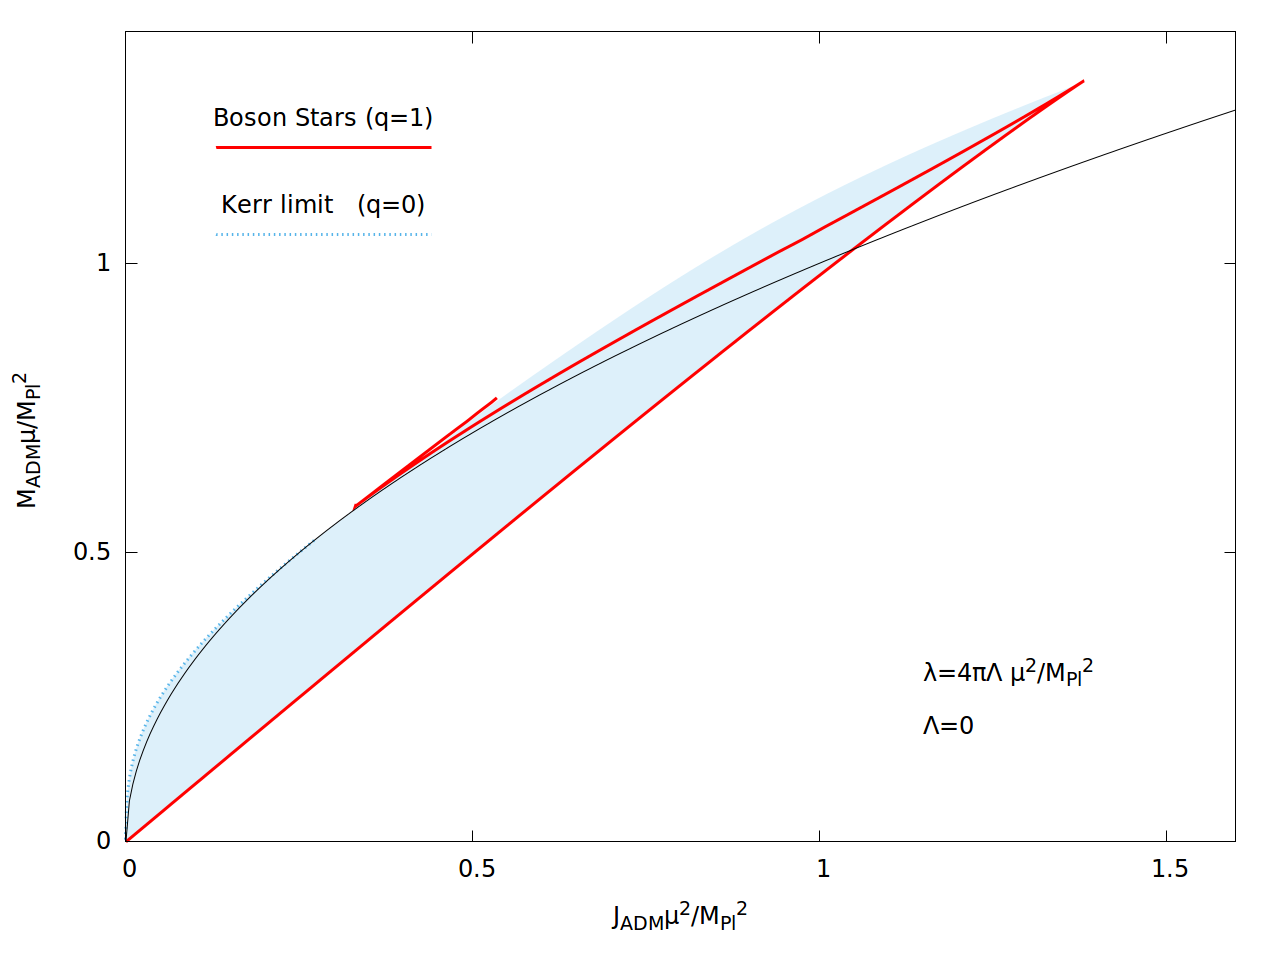
\includegraphics[width=0.48\textwidth]{papers/selfInteractions/c2=0-J-M.png}
    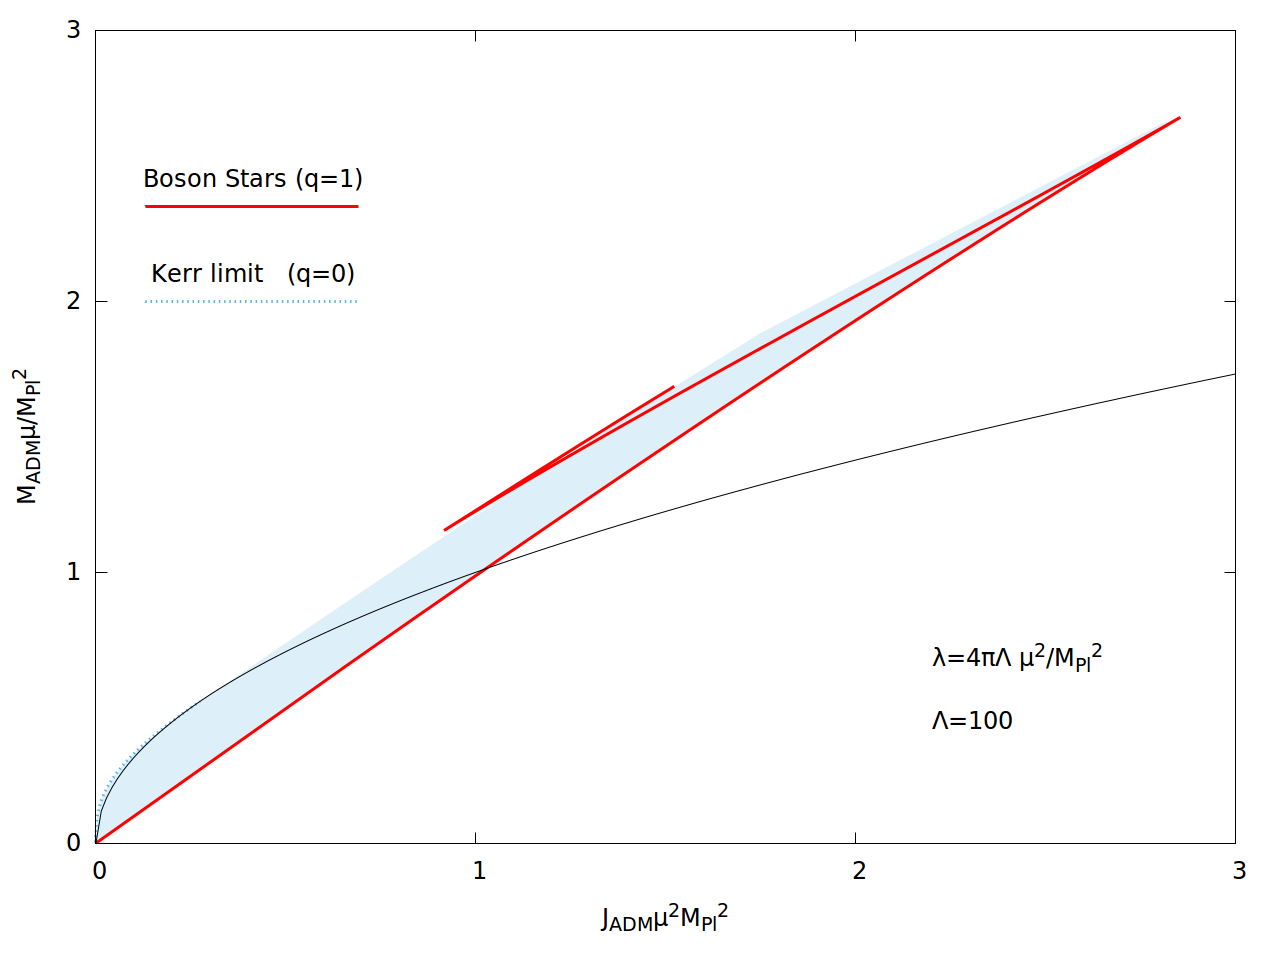
\includegraphics[width=0.48\textwidth]{papers/selfInteractions/c2=100-J-M.png}\\
    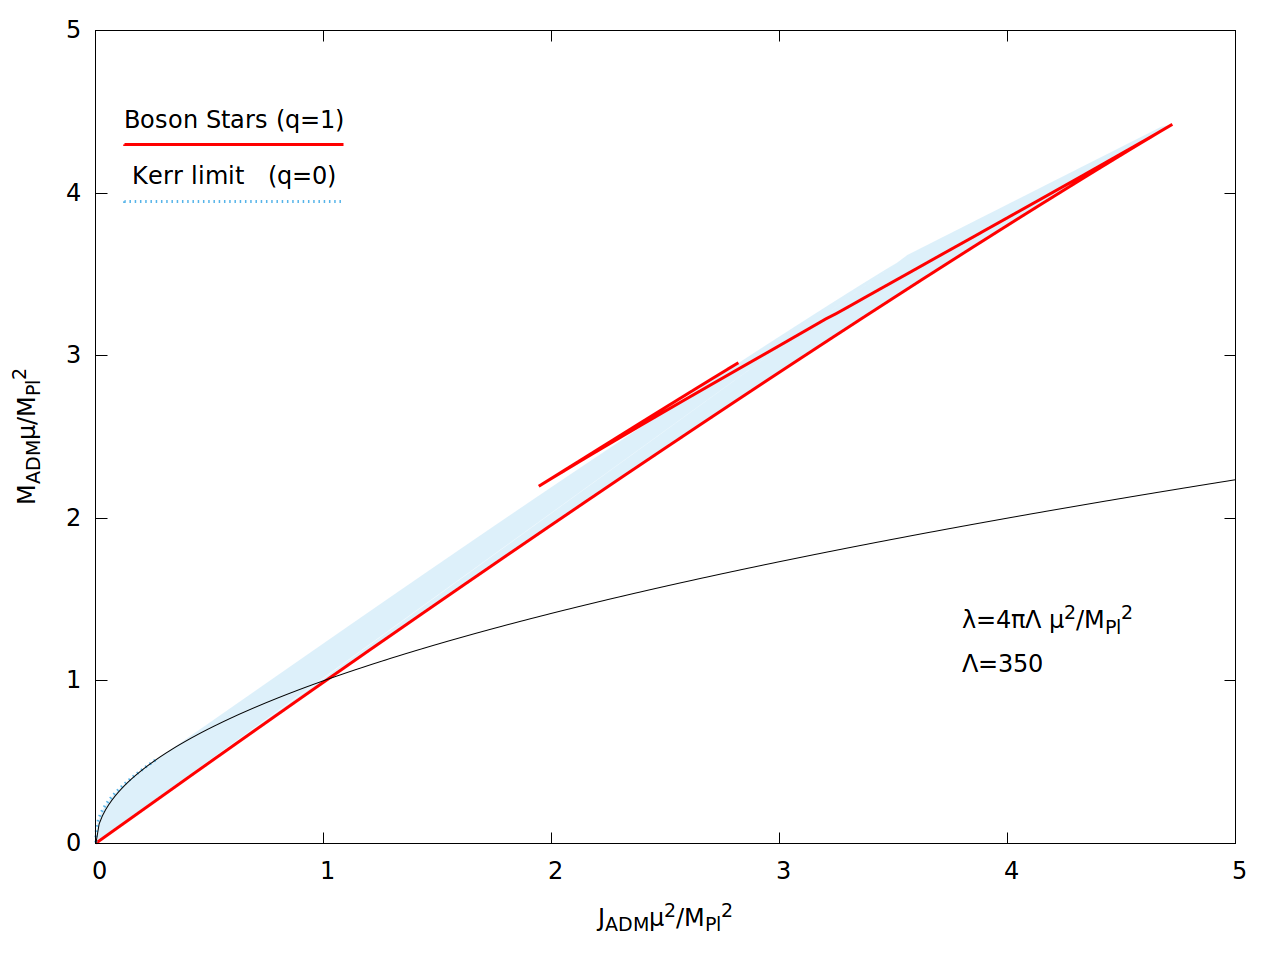
\includegraphics[width=0.48\textwidth]{papers/selfInteractions/c2=350-J-M.png}
    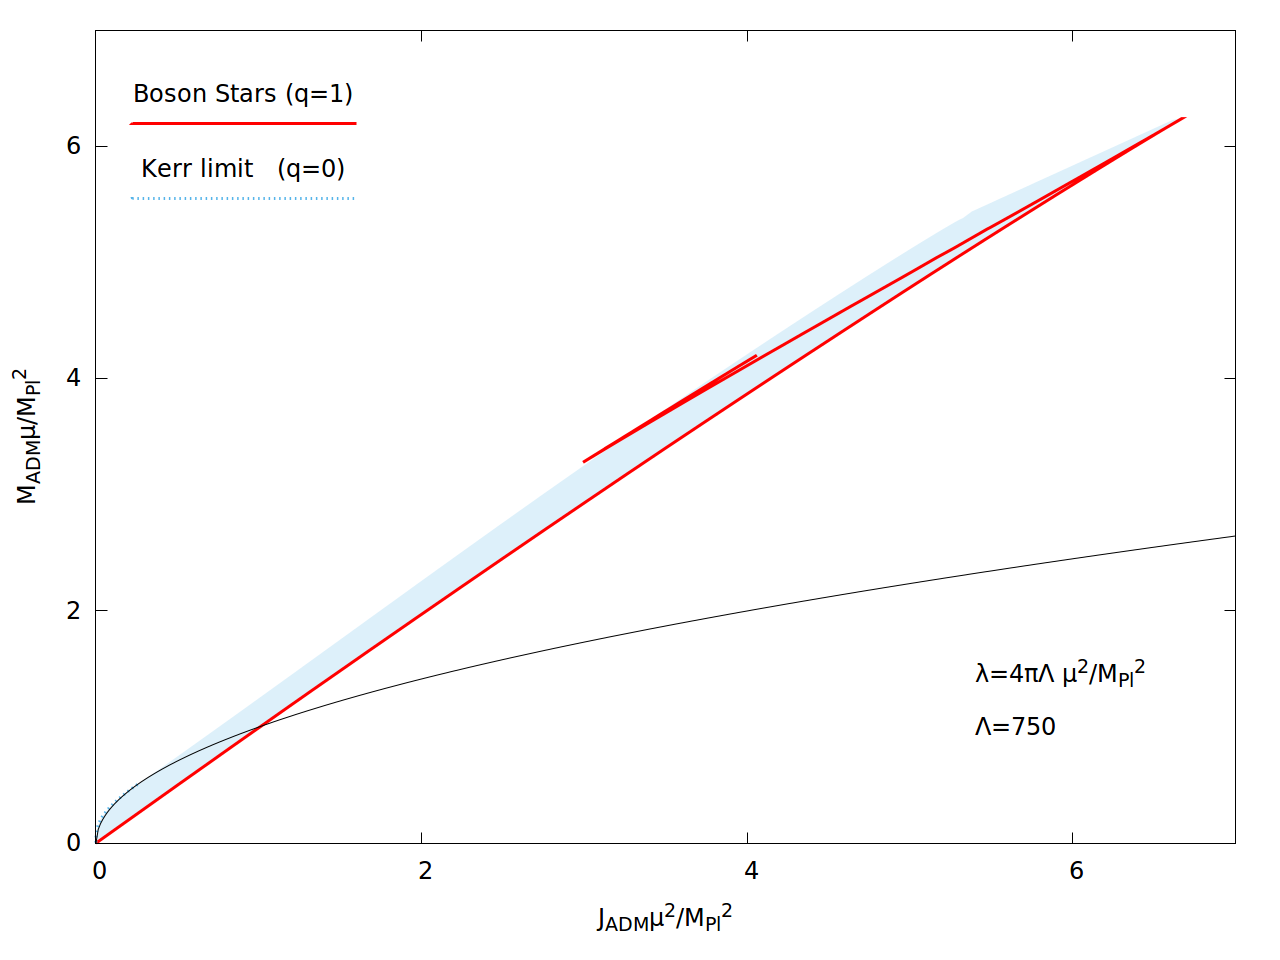
\includegraphics[width=0.48\textwidth]{papers/selfInteractions/c2=750-J-M.png}
  \end{center}
  \caption{Domain of existence of KBHsSH in an ADM mass $vs.$ ADM angular momentum diagram, for $\Lambda=0,100$ (top left and right panels) and $\Lambda=350,750$ (bottom left and right panels).}
  \label{fig:no-HBHs}
\end{figure}
 

%%%%%%%%%%%%%%%%%%%%%%%%%%%%%%%%%%%%%%%%%%%%%%%%%%%%%%%%%%%%%%%%%%%%%%%%%%%%%%%
\section{Quartic-KBHsSH: horizon quantities}
\label{sec_IV}
%%%%%%%%%%%%%%%%%%%%%%%%%%%%%%%%%%%%%%%%%%%%%%%%%%%%%%%%%%%%%%%%%%%%%%%%%%%%%%%

 
We now turn our attention to the horizon mass, $M_{\rm H}$, and angular momentum, $J_{\rm H}$. In Fig.~\ref{horizon_phase}, we display the phase space of quartic-KBHsSH, for a particular value of $\lambda$, but that illustrates the general pattern we have observed. 


\begin{figure}[h!]
  \begin{center}
    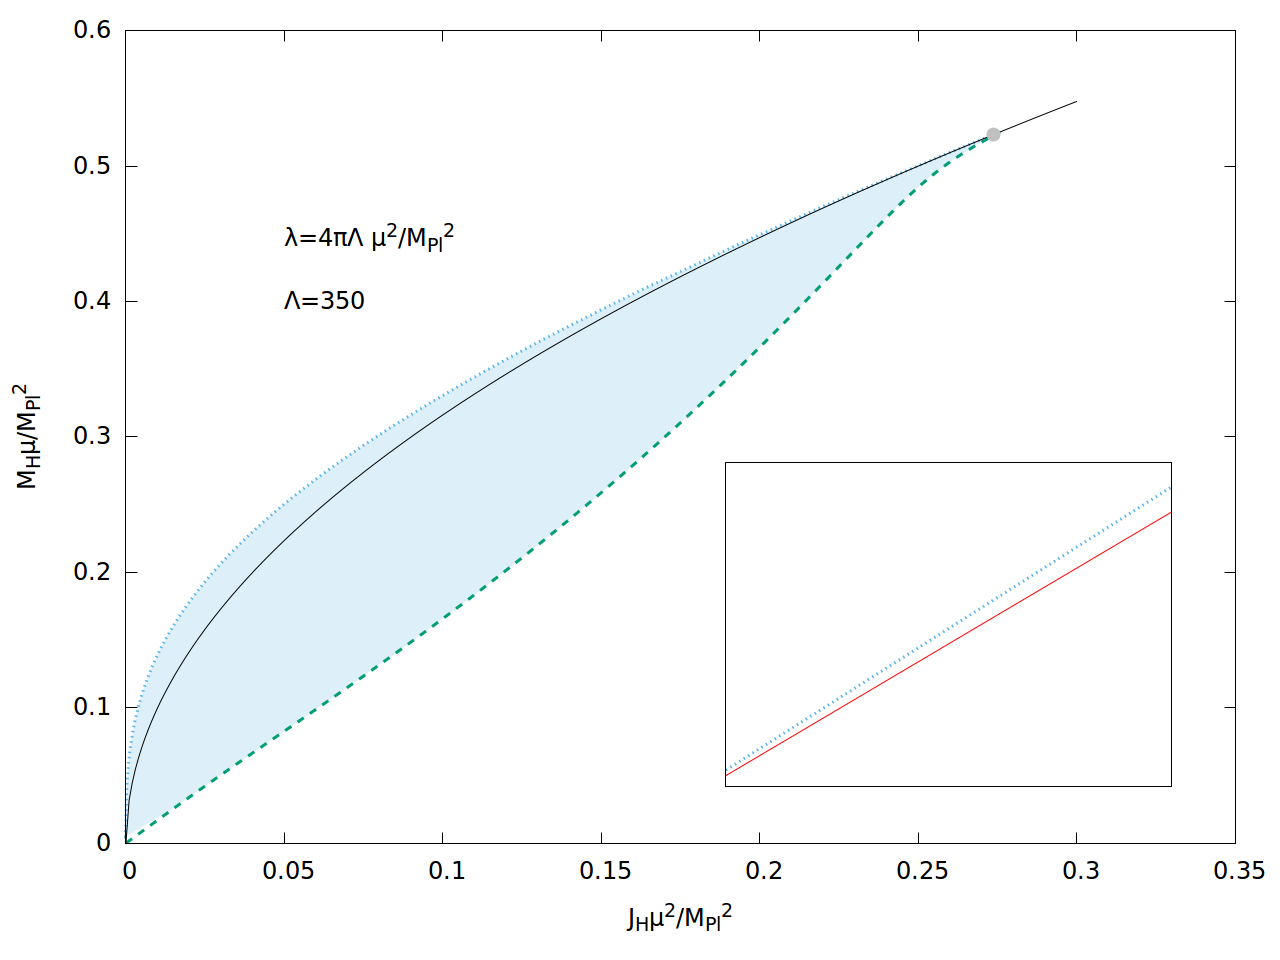
\includegraphics[width=0.7\textwidth]{papers/selfInteractions/horizon-quantities.png}
      \end{center}
  \caption{Phase space in terms of horizon quantities.}
  \label{horizon_phase}
\end{figure}

In Fig.~\ref{horizon_phase}, we can see that all solutions lie within the envelope formed by the (blue dotted) line of vacuum Kerr BHs and the (green dashed) line of extremal KBHsSH, corresponding to the blue shaded region. The salient feature we wish to emphasize is that all quartic-KBHsSH have, therefore, a \textit{lower} mass than that at the Hod point. The same pattern is observed for all other values of $\lambda$ we have studied. 


The black solid line in Fig.~\ref{horizon_phase} denotes the Kerr bound threshold, in terms of horizon quantities, $J_{\rm H}=M_{\rm H}^2$, and it can be observed that there are solutions below it, thus violating the Kerr bound in terms of horizon quantities, as was observed in~\cite{Herdeiro:2015moa} for KBHsSH without self-interactions. 

Finally, the inset of Fig.~\ref{horizon_phase} illustrates the typical pattern when starting from a given vacuum Kerr BH (on the blue dotted line) and increasing the hair, but keeping the frequency $w$ constant -- which we use as a control parameter. The corresponding points fall into the red solid line in the inset. One observes that making (vacuum) Kerr BHs hairier in this way, their horizon quantities increase, but the horizon mass increases more slowly in term of the horizon angular momentum than along the vacuum Kerr line. 


Fig.~\ref{horizon_phase} tells us that the boundary of the domain of (quartic-)KBHsSH, in the phase space constructed from horizon quantities, is composed by a curve that does not depend on $\lambda$ and the extremal hairy BHs line, that depends on $\lambda$.  As such, we study in Fig.~\ref{horizon_ratios}
the ratio between $M_H^{(\lambda)}$, $J_H^{(\lambda)}$ for extremal BHs and the corresponding values at the Hod point. We see that this ratio, as a function of the ratio for the corresponding angular momenta, does not depend strongly on $\lambda$, and in particular is always a monotonic function. Moreover, as can be seen in the inset of this same figure, the maximal mass for extremal KBHsSH is obtained at the Hod point, as all the curves approach that point from below, regardless of the value of the coupling.

\begin{figure}[h!]
  \begin{center}
    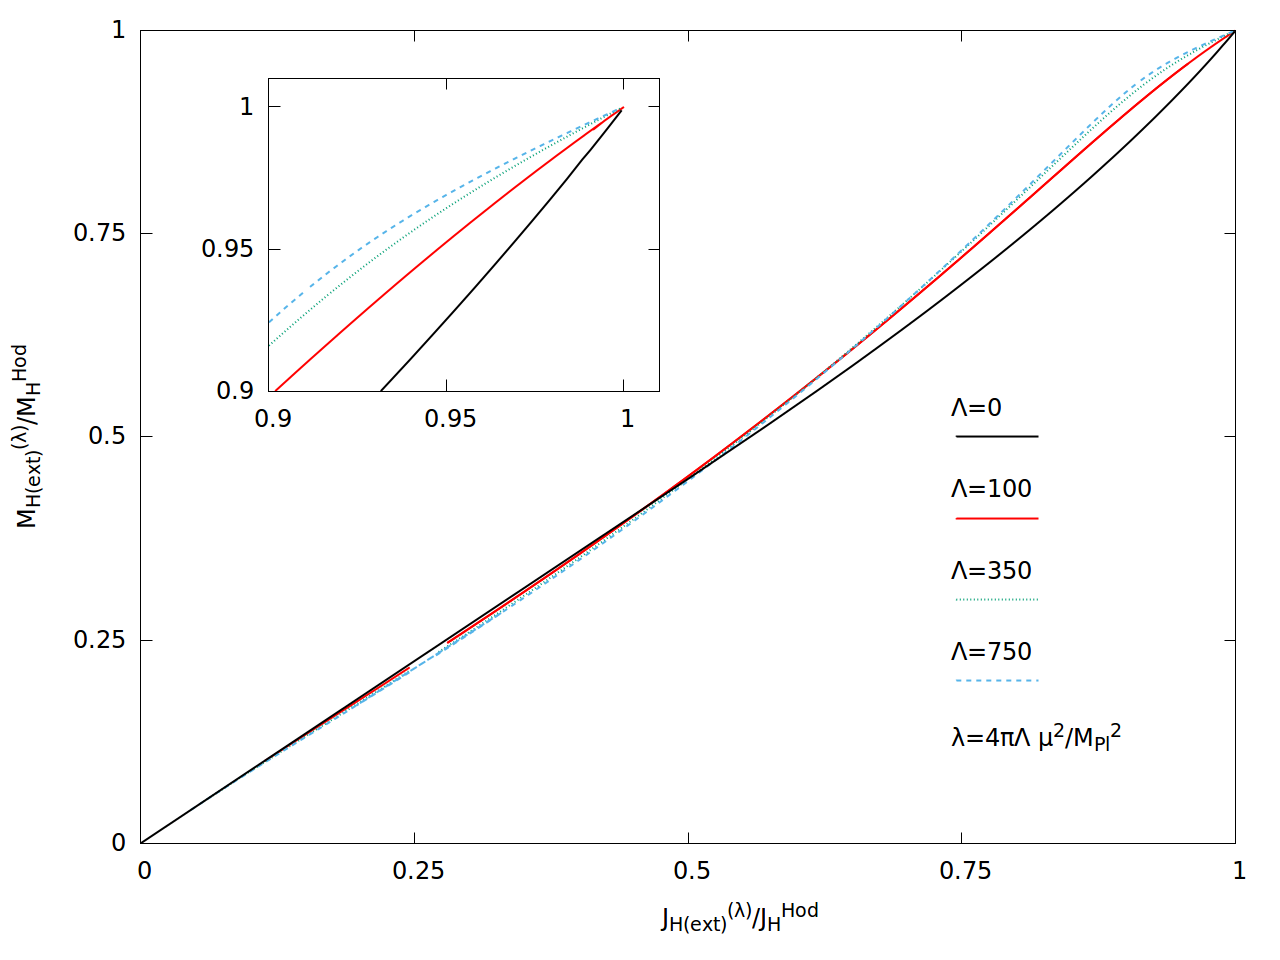
\includegraphics[width=0.7\textwidth]{papers/selfInteractions/horizon-ratios.png}
      \end{center}
      \caption{ The horizon quantities of extremal  KBHsSH and quartic-KBHsSH given in terms of the values at the Hod point, for different values of $\lambda$.}
  \label{horizon_ratios}
\end{figure}

To summarize, as the (quartic-)KBHsSH are bounded by the extremal KBHsSH line and the vacuum Kerr BH line,  and since both of these curves have their maxima at the Hod point, 
we conclude that the maximal horizon quantities are obtained at the Hod point and all 
(quartic-)KBHsSH will have horizon quantities that are
lower than those at this point.



%%%%%%%%%%%%%%%%%%%%%%%%%%%%%%%%%%%%%%%%%%%%%%%%%%%%%%%%%%%%%%%%%%%%%%%%%
\section{Discussion: universality and phenomenology}
\label{sec_V}
%%%%%%%%%%%%%%%%%%%%%%%%%%%%%%%%%%%%%%%%%%%%%%%%%%%%%%%%%%%%%%%%%%%%%%%%%%%%%%%
The main, and somehow unexpected, result in this chapter is the observation that quartic-self interactions make KBHsSH ``hairier but not heavier", in the sense of being able to increase their ADM mass but not their horizon mass, with respect to the maximal values attained in the absence of self-interactions. An immediate question is how \textit{universal} this behaviour is, if one considers a generic self-interacting scalar field theory.

To test this universality, we briefly consider a family of potentials discussed in Chapter \ref{ch:Q}.

On one hand, a systematic study of the spinning solitons 
(including the effects induced by the backreaction on the spacetime geometry) 
is given in \cite{Kleihaus:2005me}.
%As shown in Figure ??,
The results therein show that the
 generic gravitating boson stars in this theory, which we dub \textit{Q}-boson stars, follow closely the pattern for mini-boson stars and quartic-boson stars described herein; in particular 
one finds a similar, though somewhat distorted, version of the mass $vs.$ frequency diagram shown in Fig.~\ref{fig:w-vs-M-BSs}.

We have done some preliminary studies of backreacting $Q$-balls, and found families of KBHsSH with this type of self-interactions, which we dub $Q$-KBHsSH. The overall properties of these BH solutions are similar to those found herein for  quartic-KBHSSH.
In particular, the domain of existence is still bounded by the (corresponding)
curves ${\bf i)}$, ${\bf ii)}$ and ${\bf iii)}$ as defined in Section \ref{sec_III}. 
Therefore, the maximal ADM mass 
of the solutions is 
that of the corresponding $Q$-boson stars.
We remark that for the same scalar field mass, $Q$-KBHsSSH seem able to become considerably hairier than KBHsSH or quartic-KBHsSH.
%
An example of the domain of existence of $Q$-KBHsSH is presented in Fig.~\ref{qkbhsh} for the particular choice of coupling parameters used in Chapter \ref{ch:Q}.
%
\begin{figure}[h!]
  \begin{center}
     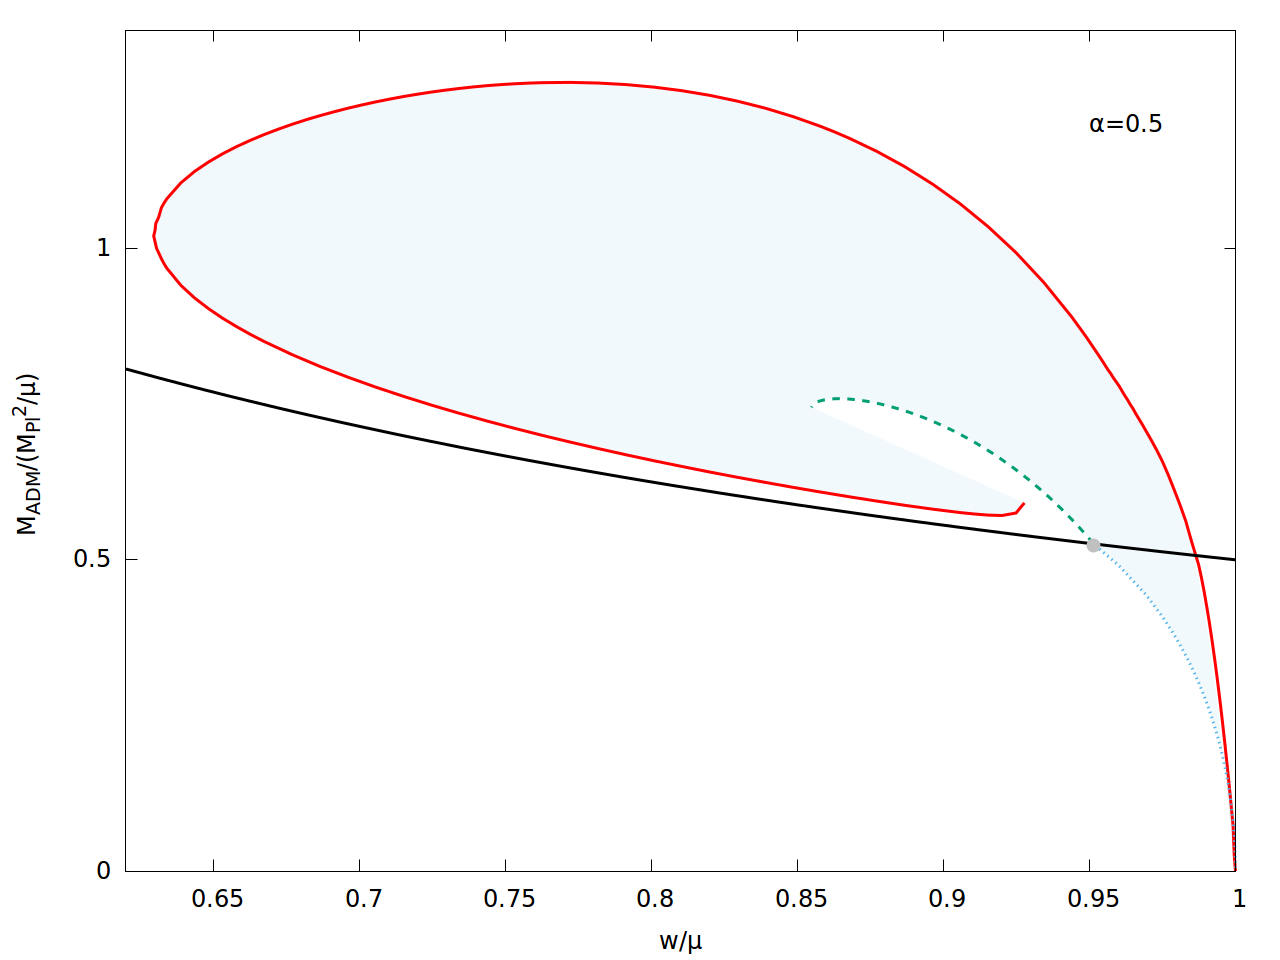
\includegraphics[width=0.7\textwidth]{papers/selfInteractions/w-vs-M-Q-a=05.png}
      \end{center}
  \caption{Domain of existence of a typical set of $Q$-KBHsSH (blue shaded region).}
  \label{qkbhsh}
\end{figure}
%


We have found that the horizon quantities
for all families of solutions studied so far,
 the pattern in 
Figs. \ref{horizon_phase} and \ref{horizon_ratios},   
is preserved.
In particular, the maximum of the horizon mass and angular momentum
are those of the (universal) Hod point - Fig.~\ref{horizon_ratios_q}

\begin{figure}[h!]
  \begin{center}
    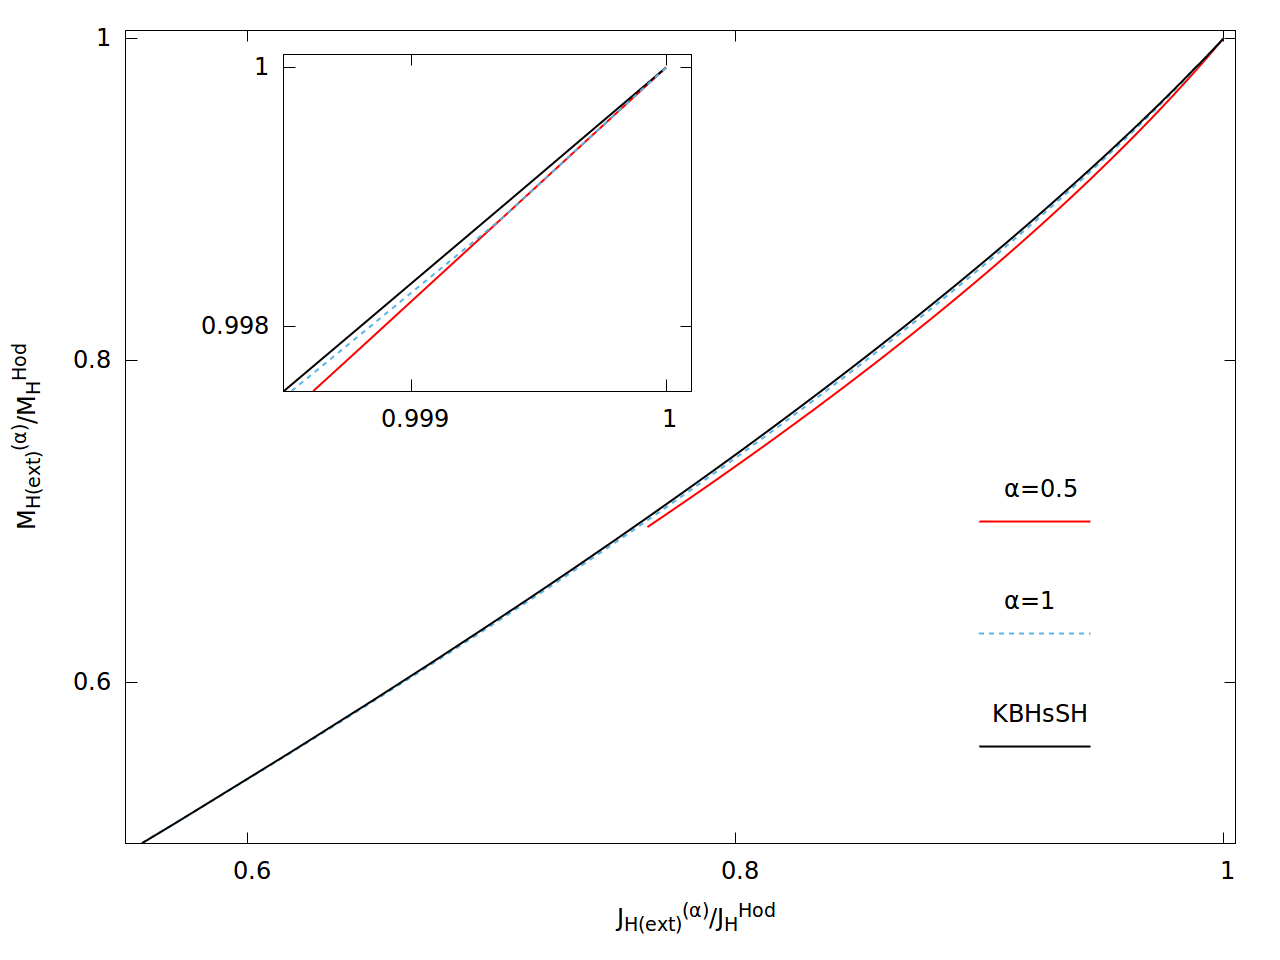
\includegraphics[width=0.7\textwidth]{papers/selfInteractions/horizon-ratios-Q.png}
      \end{center}
      \caption{ The horizon quantities of extremal  $Q$-KBHsSH given in terms of the values at the Hod point, for two different values of $\alpha$. The corresponding curve for KBHsSH without self-interactions almost overlaps with the $\alpha=1$ curve, confirming the behaviour described in the text.}
  \label{horizon_ratios_q}
\end{figure}


A final observation concerning $Q$-KBHsSH, that follows from our numerical data 
is that 
when the coupling 
constant  $\alpha$ is increased,
the solutions tend to those with a free scalar field in \cite{Herdeiro:2014goa}. 
In fact, 
following the arguments in \cite{Kleihaus:2005me}, one can show that 
for large values of $\alpha$, all higher order terms in the scalar field potential become irrelevant
and, as $\alpha\to \infty$, one recovers the solutions of a model with a complex scalar field  
possessing a quadratic potential only. In fact, this feature starts to manifest already for $\alpha$  of order 1. This provides further evidence for the universality of the ``hairier but not heavier" behaviour.

\bigskip

The result of this chapter is the following: the maximum horizon mass, $M^{\rm max}_H$, for KBHsSH (with or without self-interactions) is attained at a particular configuration we dub the \textit{Hod point}, corresponding to the extremal (vacuum) Kerr BH obtained in the vanishing hair limit, and precisely one of the points studied in~\cite{Hod:2012px}.
For KBHsSH this maximal mass obeys the same form as \eqref{mini},
\begin{equation}
  M_{\rm H}^{\rm max}\simeq \alpha_{\rm Hod} \frac{M_{\rm Pl}^2}{\mu}\simeq \alpha_{\rm Hod} \, 10^{-19}M_\odot\left(\frac{\rm GeV}{\mu}\right)\ , 
\label{hodpoint}
\end{equation}
 but with the constant $\alpha_{\rm Hod}<\alpha_{\rm BS}$. For instance, for $m=1;2$, $\alpha_{\rm Hod}=0.526; 1.165$. 

\bigskip

Since the maximal horizon mass behaves as in Eq. \eqref{hodpoint}, if the ``hairier" but not ``heavier" property is universal and holds regardless of the scalar field theory, then KBHsSH with a trapped region with astrophysical masses can only exist if ultra-light scalars occur in Nature. This type of hairy BHs would be, therefore, a distinct observational signature of such beyond the Standard Model particles.

\bigskip

In the next chapter, we will study massive vector hair around Kerr black holes.
%
%
%
% \vspace{0.5cm} 
%  %%%%%%%%%%%%%%%%%%%%%%%%%%%%%%%%%%%%%%%%%%%%%%%%%%%%%%%%%%%%%%%%%%%
% \noindent
% \section*{Acknowledgements}
% C. H. and E. R. acknowledge funding from the FCT-IF programme. H.R. is supported by the grant PD/BD/109532/2015 under the MAP-Fis Ph.D. programme. This work was partially supported by the NRHEPÐ295189
% FP7-PEOPLE-2011-IRSES Grant, by FCT via project No.
% PTDC/FIS/116625/2010 and by the CIDMA strategic project UID/MAT/04106/2013. Computations were performed at the Blafis cluster, in Aveiro University.
%  
\chapter{Kerr black holes with Proca hair}
\label{ch:proca}

\epigraph{``\emph{
Ein sat hún úti \\
þá er inn aldni kom \\
yggjungur ása \\
og í augu leit: \\
„Hvers fregnið mig? \\
Hví freistið mín?“ \\
Allt veit eg, Óðinn, \\
hvar þú auga falt, \\
í inum mæra \\
Mímisbrunni. \\
Drekkur mjöð Mímir \\
morgun hverjan \\
af veði Valföðurs. \\
Vituð ér enn eða hvað? 
} 
''}{28th verse of Völuspá}


%%%%%%%%%%%%%%%%%%%%%%%%%%%%%%%%%%%%%%%%%%%%%%%%%%%%%%%%%%%%%%%%%%%%%%%%%%%%%%%
\section{Introduction}
% %%%%%%%%%%%%%%%%%%%%%%%%%%%%%%%%%%%%%%%%%%%%%%%%%%%%%%%%%%%%%%%%%%%%%%%%%%%%%%%
%  
% In vacuum General Relativity (GR) black holes (BH) are remarkably simple. The Carter-Robinson theorem~\cite{Carter:1971zc,Robinson:1975bv}, supplemented by the rigidity theorem~\cite{Hawking:1971vc,Racz:1995nh}, established that asymptotically flat, stationary, non-singular (on and outside an event horizon)  \textit{vacuum} BHs of GR have \textit{only} 
% two degrees of freedom -- see~\cite{Chrusciel:2012jk} for a review.  
%
% The most general BH solution in this context is the Kerr metric~\cite{Kerr:1963ud} and the two degrees of freedom are the ADM mass, $M$, and angular momentum, $J$, both of which can be determined by an observer at infinity. 
%
% The natural question of how this result generalizes in the presence of matter led to the \textit{no-hair} hypothesis~\cite{Ruffini:1971bza}: regardless of the matter involved, the end-point of gravitational collapse -- in GR and in an astrophysical context -- is characterized solely by conserved charges associated to Gauss laws, including $M,J$, and no further parameters (\textit{hair}). Thus, an observer at infinity should be able to fully compute all relevant ``charges" of an equilibrium BH.
%
% Evidence in favour of this hypothesis has been presented in terms of \textit{no-hair theorems} for particular matter models in GR. A collection of such theorems for the much studied case of scalar matter can be found in the recent review~\cite{Herdeiro:2015waa}. Of relevance for the present paper, Bekenstein established a no-Proca hair theorem for stationary BH solutions of Einstein's gravity minimally coupled to one (or more) real, Abelian Proca field~\cite{Bekenstein:1971hc,Bekenstein:1972ky}, which will be reviewed in Section~\ref{sec_nohair1}. 
%
%
%
% Evidence against the no-hair hypothesis in asymptotically flat spacetimes, on the other hand, has been presented in the form of hairy BH solutions, starting with the pioneering examples in Yang-Mills theory~\cite{Volkov:1998cc} (see also the reviews~\cite{Bizon:1994dh,Bekenstein:1996pn,Herdeiro:2015waa,Volkov:2016ehx}). 
% Such counter-examples, however, typically either 
% 1) violate some energy condition ($e.g.$~\cite{Nucamendi:1995ex,Bechmann:1995sa,Anabalon:2013qua,Anabalon:2012ih,Cadoni:2015gfa}); or 
% 2) have non-minimal couplings between matter and geometry ($e.g.$~\cite{Bekenstein:1975ts,Bekenstein:1974sf,BBM,Sotiriou:2014pfa,Sotiriou:2013qea,Babichev:2013cya}); or 
% 3) have non-canonical/non-linear kinetic terms ($e.g.$~\cite{Luckock:1986tr,Luckock,Bronnikov:2005gm,Radu:2011uj}); or 
% 4) the hair is not independent of other fields, such as an electromagnetic field (secondary hair, $e.g.$~\cite{Gibbons:1987ps,Gibbons:1982ih}); or 
% 5) involve higher curvature terms 
% ($e.g$~\cite{Kanti:1995vq,Ayzenberg:2014aka,Kleihaus:2011tg,Kleihaus:2015aje,Pani:2011gy,Pani:2009wy,Alexander:2009tp,Yunes:2009hc}); or 
% 6) several of the above. It is unclear, moreover, if any of these counter-examples violates the \textit{dynamical spirit} of the no-hair hypothesis; that is, if there are dynamically stable hairy BHs that can be the end-point (or be sufficiently long lived) in a dynamical evolution.
%
% \bigskip
%
% In a qualitatively novel development, a class of BH solutions with scalar hair was found in 2014 bifurcating from the Kerr metric~\cite{Herdeiro:2014goa}: \textit{Kerr BHs with scalar hair} (KBHsSH).
% %
%  These are solutions of the simple model
%  \begin{equation}
% \label{actionscalar}
% S=\int  d^4x \sqrt{-g}\left[ \frac{R}{16\pi G}
%    -\frac{g^{\alpha\beta}}{2} \left( \Psi_{, \, \alpha}^* \Psi_{, \, \beta} + \Psi _
% {, \, \beta}^* \Psi _{, \, \alpha} \right) - \mu^2 \Psi^*\Psi
% %( \left| \Phi \right|) 
%  \right]  \ ,
% \end{equation}
% that 1) obey all energy conditions; 2) have minimal couplings with the geometry; 3) have canonical kinetic terms; 4) have an independent (primary) hair; 5) exist in GR, without higher curvature terms. KBHsSH, moreover, are asymptotically flat, regular on and outside the event horizon, reduce to (specific) Kerr solutions in the limit of vanishing hair, and to gravitating solitons known as \textit{boson stars}~\cite{Schunck:2003kk,Liebling:2012fv} in the limit of vanishing horizon. The scalar hair is described by an independent  conserved Noether charge \textit{but without} an associated Gauss law. Thus, an observer at infinity cannot determine this charge -- which must be computed by a volume integral -- and hence does not have access to all the relevant spacetime charges.  
%
For both KBHsSH and the generalization considered in Chapter \ref{ch:SI}, the matter content was a massive complex scalar field.
As we have discussed the existence of these solutions is tied to the phenomena of superradiance.
This connection led to the suggestion that there is a more general mechanism at play~\cite{Herdeiro:2014goa,Herdeiro:2014ima} (see also~\cite{Herdeiro:2015waa,Herdeiro:2015gia}): 
{\bf Conjecture:}
\begin{description}
\item[1)] If a ``hairless" stationary BH spacetime $(\mathcal{M}_0,{\bf g_0})$ is afflicted by superradiant instabilities triggered by a given test field $\mathcal{F}$;
\item[2)] If the field modes at the threshold of the instability (zero modes), $\mathcal{F}_t$, yield an energy-momentum tensor $\mathcal{T}(\mathcal{F}_t,\mathcal{F}_t)$ which is time-independent $\mathcal{L}_{\bf k}\mathcal{T}(\mathcal{F}_t,\mathcal{F}_t)=0$, where ${\bf k}$ is the time-like Killing vector field (at infinity) that preserves the metric $\mathcal{L}_{\bf k}{\bf g_0}=0$;
\item[Then:] there is a new family of stationary BH ``hairy solutions" bifurcating from $(\mathcal{M}_0,{\bf g_0})$, denoted by $(\mathcal{M}_\mathcal{F},{\bf g_\mathcal{F}})$. Actually, $(\mathcal{M}_\mathcal{F},{\bf g_\mathcal{F}})$ may be a countable set of families.
\end{description}
As we have seen, in the case of KBHsSH, one encounters a family with three continuous and two discrete degrees of freedom.

As further evidence for the above conjecture we consider now 
Einstein's gravity minimally coupled to Abelian Proca fields, hereafter referred simply as Proca fields\footnote{Gravitating \textit{non-Abelian} ($SU(2)$) Proca fields have been studied in \cite{Greene:1992fw}, wherein spherically symmetric solitons and BHs have been discussed. The properties of these solutions are rather distinct from the solutions discussed in this chapter and, moreover, the former have not been generalized to include rotation.}. 
Massive Proca fields trigger, in much the same way as massive scalar fields, 
superradiant instabilities of Kerr BHs -- see~\cite{Pani:2012vp,Pani:2012bp,Witek:2012tr} 
for recent studies of Proca-induced superradiant instabilities in asymptotically flat BHs. 

In this chapter, we will start by looking at the Einstein-(complex)-Proca model.
That is, we will consider a complex Proca field coupled to the Einstein equations.
We will then very briefly review some no-Proca-hair theorems.
After that, we will construct first stationary Proca clouds around Kerr black holes and second review spinning Proca stars.
Just as for KBHsSH, these families of solutions form a part of the boundary for the hairy black hole solutions.
Finally, we will present Kerr black holes with Proca hair (KBHsPH) and discuss some of their properties.

 %%%%%%%%%%%%%%%%%%%%%%%%%%%%%%%%%%%%%%%%%%%%%%%%%%%%%%%%%%%%%%%%%%%%%%%%%%%%%%%
\section{Einstein--complex-Proca model}
\label{Psec_model}
%%%%%%%%%%%%%%%%%%%%%%%%%%%%%%%%%%%%%%%%%%%%%%%%%%%%%%%%%%%%%%%%%%%%%%%%%%%%%%% 
The field equations for a massive vector field were introduced by A. Proca~\cite{Proca} in the 1930s. Much more recently, gravitating Proca fields have been discussed by various authors -- see $e.g.$~\cite{Rosen:1994rq,Obukhov:1999ed,Toussaint:1999zz}. Here, we shall consider  two real Proca fields, both with mass $\mu$, but our discussion can be easily generalized to an arbitrary even number of real Proca fields (or an arbitrary number of complex ones). 
The two fields are described by the potential 1-forms $A^{(i)}$, $i=1,2$, and field strengths $F^{(i)}=dA^{(i)}$. It is convenient to organize them into a single complex Proca field:
\begin{equation}
\mathcal{A}=A^{(1)}+iA^{(2)} \ , \qquad \mathcal{F}=F^{(1)}+iF^{(2)} \ .
\end{equation}
We denote the complex conjugate by an overbar,
\begin{equation}
\bar{\mathcal{A}}=A^{(1)}-iA^{(2)} \ , \qquad \bar{\mathcal{F}}=F^{(1)}-iF^{(2)} \ .
\end{equation}
Considering that the two Proca fields do not couple to each other and couple minimally to gravity, one obtains the minimal Einstein--complex-Proca model, which is  
described by the action:
\begin{equation}
\label{Procaaction}
\mathcal{S}=\int d^4x \sqrt{-g}\left(\frac{1}{16 \pi  G}R
-\frac{1}{4}\mathcal{F}_{ab}\bar{\mathcal{F}}^{ab}
-\frac{1}{2}\mu^2\mathcal{A}_a\bar{\mathcal{A}}^a\right) \ .
\end{equation}
This (or its version with $A_a$ real) 
is the action considered by previous studies of the Einstein-Proca model, see
$e.g.$ refs. \cite{Rosen:1994rq,Vuille:2002qz}.\footnote{We remark that these works did not succeed in finding regular particle-like solutions or BHs with Proca hair.}

Varying Eq. (\ref{Procaaction}) with respect to the potential $A_a$ yields the Proca field equations
\begin{equation}
\nabla_a\mathcal{F}^{ab}=\mu^2 \mathcal{A}^b \ .
\label{procafe}
\end{equation}
Observe that these equations \textit{completely} determine $ \mathcal{A}^b$ once $\mathcal{F}^{ab}$ is known. Thus, the Proca potential is not subject to gauge transformations, unlike the Maxwell potential, and it is as physical as the field strength. In particular \eqref{procafe} imply the Lorentz condition, thus a dynamical requirement, rather than a gauge choice:
\begin{equation}
\nabla_a\mathcal{A}^a = 0 \ .
\label{lorentz}
\end{equation}


As usual, the Einstein equations are found by taking the variation of
(\ref{Procaaction}) $w.r.t.$ the metric tensor $g_{ab}$
\begin{equation}
R_{ab}-\frac{1}{2}R g_{ab}=8 \pi G T_{ab} \ ,
\label{Einstein-eqs}
\end{equation}
where the energy-momentum tensor reads:
\begin{eqnarray}
T_{ab}=\frac{1}{2}
( \mathcal{F}_{ac}\bar{\mathcal{F}}_{bd}
+\bar{\mathcal{F}}_{ac} \mathcal{F}_{bd}
)g^{cd}
-\frac{1}{4}g_{ab}\mathcal{F}_{ce}\bar{\mathcal{F}}^{ce}+\frac{1}{2}\mu^2\left[  
\mathcal{A}_{a}\bar{\mathcal{A}}_{b}
+\bar{\mathcal{A}}_{a}\mathcal{A}_{b}
-g_{ab} \mathcal{A}_c\bar{\mathcal{A}}^c\right]\ . \ \ \ \ \ \ \  \ 
\label{procaemt}
\end{eqnarray}

The action possesses a global $U(1)$ symmetry, since it is invariant under the transformation 
$\mathcal{A}_b\rightarrow e^{i\chi}\mathcal{A}_b$, with $\chi$ constant; 
this implies the existence of a  4-current, 
%
\begin{equation}
\label{j}
j^a=\frac{i}{2}\left[\bar{\mathcal{F}}^{ab}\mathcal{A}_b-\mathcal{F}^{ab}\bar{\mathcal{A}}_b\right] \ ,
\end{equation}
which is conserved by virtue of the field equations (\ref{procafe}): $\nabla_a j^a=0$. Consequently, there exists a Noether charge, $Q$, obtained integrating the temporal component of the 4-current on a space-like slice $\Sigma$:
\begin{equation}
Q=\int_\Sigma d^3x j^0 \ .
\label{Pq}
\end{equation}
We emphasize that unlike the massless limit of the theory, wherein the global symmetry becomes local, the last integral cannot be converted into a surface integral. In other words, there is no Gauss law.


 
 %%%%%%%%%%%%%%%%%%%%%%%%%%%%%%%%%%%%%%%%%%%%%%%%%%%%%%%%%%%%%%%%%%%%%%%%%%%%%%%
\section{No Proca-hair theorems}
\label{sec_nohair}
%%%%%%%%%%%%%%%%%%%%%%%%%%%%%%%%%%%%%%%%%%%%%%%%%%%%%%%%%%%%%%%%%%%%%%%%%%%%
If one considers Maxwell's equations for a test field with a spherically symmetric ansatz (a purely radial electric field) on the Schwarzschild background one finds a regular solution on and outside the Schwarzschild horizon ($cf.$ Section 2.1 in~\cite{Herdeiro:2015waa}). This is a smoking gun that a spherically symmetric field can be added, non-linearly, to the Schwarzschild solution, which indeed yields the well-known Reissner-Nordstr\"om solution. 
Adding a mass term to the Maxwell field -- hence converting it into a Proca field -- drastically alters the behaviour of the test field solution: it is not possible to find a solution which is both finite at the horizon and at spatial infinity, no matter how small $\mu$ is. 
In particular, for the asymptotically (exponentially) decaying solution, the Proca potential squared diverges at the horizon~\cite{Gottlieb:1984jg}.
Thus, requiring any amount of Proca field in equilibrium outside the horizon implies an infinite pile up of Proca invariants at the horizon.
This behaviour parallels that of a scalar field (massless or massive) discussed in~\cite{Herdeiro:2015waa} and it is intimately connected with the existence/absence of a Gauss law for the Maxwell/Proca field.
Moreover, it shows one cannot find a regular, spherically symmetric BH solution with Proca (time-independent) hair bifurcating from the Schwarzschild solution.

Just as with KBHsSH, a key assumption in finding Kerr black holes with Proca hair is to violate the assumption of many no-hair theorems, many of which were put forth by Bekenstein\cite{Bekenstein:1971hc,Bekenstein:1972ky}, that the field inherits the isometries of the background.
In \cite{Herdeiro:2016tmi}, it was shown that even dropping the symmetry inheritance assumption one can establish a no-hair theorem, for \textit{spherically symmetric} BHs.
This is compatible with the KBHsPH solutions discussed in this chapter, which are stationary and axi-symmetric, and shows that these solutions cannot have a static limit,
as can be seen from the domain of existence of KBHsPH, $cf.$ Section~\ref{subsec_III}.

%
% %%%%%%%%%%%%%%%%%%%%%%%%%%%%%%%%%%%
% \subsection{Bekenstein's theorem}
% \label{sec_nohair1}
% %%%%%%%%%%%%%%%%%%%%%%%%%%%%%%%%%%%%%%%%%%%%%%%%%%%%%%%%%%%%%%%%%%%%%%%%%%%%
% Following Bekenstein~\cite{Bekenstein:1971hc,Bekenstein:1972ky}, we consider a rotating, stationary, asymptotically flat BH spacetime. For matter obeying the null energy condition, the rigidity theorem implies that the spacetime is also axi-symmetric~\cite{Hawking:1971vc}. We write the spacetime metric in coordinates adapted to these symmetries $(t,r,\theta,\phi)$, so that the two Killing vector fields read ${\bf k}=\partial_t$, ${\bf m}=\partial_\phi$.
%
%
% For simplicity we consider the Proca field to be real. But the proof generalizes straightforwardly for an arbitrary number of real Proca fields, and in particular for a complex Proca field. We denote the real Proca potential and field strength as $A_\alpha$ and $F_{\alpha\beta}$, respectively. We assume that this field inherits the spacetime symmetries. In particular for the coordinates chosen above 
% this means that: 
% \begin{equation}
% \mathcal{L}_{\bf k} A_\alpha=\mathcal{L}_{\bf m} A_\alpha=0=\mathcal{L}_{\bf k} F_{\alpha\beta}=\mathcal{L}_{\bf m} F_{\alpha\beta} \ .
% \label{symmetriesaf}
% \end{equation}
%
% The proof proceeds as follows. We contract the Proca equation $\nabla_\alpha F^{\alpha\beta}=\mu^2 A^\beta$ with $A_\beta$ and integrate over the BH exterior space-time:
% \begin{equation}
% \int d^4x\sqrt{-g}\left[A_\beta\nabla_\alpha F^{\alpha\beta}-\mu^2 A_\beta A^\beta\right]=0 \ .
% \end{equation}
% Next, integrating the first term by parts:
% \begin{equation}
% \int d^4x\sqrt{-g}\left[\frac{F_{\alpha\beta} F^{\alpha\beta}}{2}+\mu^2 A_\beta A^\beta\right]-\int_{\mathcal{H}}d^3\sigma n^\alpha A_\beta F_{\alpha}^{\ \beta}=0 \ ,
% \label{bek1}
% \end{equation}
% where the boundary term is computed on the (spatial section of the) horizon, $\mathcal{H}$, and the other boundary term (at infinity) vanishes since the Proca field falls off exponentially fast.
%
% Now we argue that the boundary term in  \eqref{bek1} is zero. To do so, we first observe that defining $b_\alpha\equiv A_\beta F_{\alpha}^{\ \beta}$, then $b_t=0=b_\phi$. This results from the symmetries imposed, which imply $A_r=A_\theta=F_{r\theta}=F_{t\phi}=0$.\footnote{$F_{t\phi}=0$ follows immediately from~\eqref{symmetriesaf}. Non-vanishing $A_r,A_\theta,F_{r\theta}$ would imply non vanishing components $T_{tr}$ and $T_{t\theta}$ of the energy momentum tensor~\eqref{procaemt}, which are incompatible with the symmetries of the problem.} 
% Since, the event horizon of a stationary, asymptotically flat spacetime is a Killing horizon, the normal to $\mathcal{H}$, $n^\alpha$, 
% is a linear combination of the Killing vector fields. Then $n^\alpha A_\beta F_{\alpha}^{\ \beta}=0$. 
% %
% We conclude that\footnote{We are implicitly assuming that $d^3\sigma$ and $A_\alpha,F_{\alpha\beta}$ are finite on $\mathcal{H}$. This assumption actually breaks down for the massless case (Maxwell field) due to gauge invariance.}
% \begin{equation}
% \int d^4x\sqrt{-g}\left[\frac{F_{\alpha\beta} F^{\alpha\beta}}{2}+\mu^2 A_\beta A^\beta\right]=0 \ .
% \label{bek3}
% \end{equation}
%
% Contrary to the scalar field case (see $e.g.$~\cite{Herdeiro:2015waa}) this integrand is not positive definite. Thus, a further argument is necessary, which can be constructed by using an orthonormal basis, which we denote as $\{ {\bf e}^{\underline{t}},{\bf e}^{\underline{r}},{\bf e}^{\underline{\theta}},{\bf e}^{\underline{\phi}}\}$. Flat (underlined) indices are raised and lowered with the standard Cartesian Minkowski metric. Taking into account the allowed components by symmetry of the Proca potential and field strength, \eqref{bek3} becomes:
% \begin{equation}
% \begin{array}{l}
% \displaystyle{\int d^4x\sqrt{-g}\left[(F_{\underline{t}\underline{r}})^2+(F_{\underline{t}\underline{\theta}})^2+(A_{\underline{t}})^2\right]} \displaystyle{=\int d^4x\sqrt{-g}\left[(F_{\underline{\phi}\underline{r}})^2+(F_{\underline{\phi}\underline{\theta}})^2+(A_{\underline{\phi}})^2\right]} \ .
% \end{array}
% \label{procaproof}
% \end{equation}
% Analysing the time-reversal invariance of the Proca equation, shows that $\{F_{\underline{t}\underline{r}},F_{\underline{t}\underline{\theta}},A_{\underline{t}}\}$ are even, whereas $\{F_{\underline{\phi}\underline{r}},F_{\underline{\phi}\underline{\theta}},A_{\underline{\phi}}\}$ are odd, under time-reversal. Thus, expanding the Proca potential and field strength in a power series of the angular momentum of the background, the first (second) set of field/potential components contains only even (odd) powers. The zeroth order terms only get contributions from the left hand side of \eqref{procaproof}; since the corresponding integrand is strictly positive and the integral is zero, the zeroth order terms must vanish. Then, the first order terms only get contributions from the right hand side of \eqref{procaproof}; since the corresponding integrand is strictly positive and the integral is zero, the first order terms must vanish. In this way one shows iteratively that the Proca field/potential must vanish, and hence there is no Proca hair. 
% Observe that this theorem did not use the Einstein equations.
%
% A different proof of the no Proca-hair theorem, possibly including a cosmological constant  and making use of the Einstein equations, 
% has been given in \cite{Bhattacharya:2011dq}.
%
%
%
%
%  %%%%%%%%%%%%%%%%%%%%%%%%%%%%%%%%%%%%%%%%%%%%%%%%%%%%%%%%%%%%%%%%%%%%%%%%%%%%%%%
% \subsection{A modified Pe\~{n}a--Sudarsky theorem}
% \label{sec_nohair2}
% %%%%%%%%%%%%%%%%%%%%%%%%%%%%%%%%%%%%%%%%%%%%%%%%%%%%%%%%%%%%%%%%%%%%%%%%%%%%
% The theorem of the previous subsection relied on the symmetry inheritance of the spacetime isometries by the Proca field. In particular the stationarity of the geometry implied a time-independence of the Proca potential/field. Recently, however, gravitating solitons composed by self-gravitating Proca fields were found by allowing the complex Proca field to have a \textit{harmonic time dependence}: Proca stars~\cite{Brito:2015pxa}. This time-dependence vanishes at the level of the energy momentum tensor and it is therefore compatible with a stationary geometry (see~\cite{Smolic:2015txa} for recent discussions of symmetry inheritance). Thus one may wonder if allowing the Proca field to have such harmonic time dependence allows for BHs with Proca hair. 
%
% The situation just described parallels closely the well-known picture for complex scalar fields. The existence of scalar boson stars led Pe\~{n}a and Sudarsky to consider the possibility of spherically symmetric BH geometries with a scalar field possessing a harmonic time dependence. In this setup it was possible to establish a no-scalar-hair theorem, ruling out BHs with scalar hair even if the hair has such harmonic time-dependence~\cite{Pena:1997cy}. In the following we shall establish a no-Proca-hair theorem, allowing the complex Proca field to have a harmonic time dependence, for the case of spherical symmetry, by using a modified version of the arguments in~\cite{Pena:1997cy}. 
%
% We consider a spherically symmetric line element with the parametrization (see $e.g.$~\cite{Brito:2015pxa}):
% %
% \begin{equation}
% ds^2=-\sigma^2(r)N(r)dt^2+\frac{dr^2}{N(r)}+r^2d\Omega_2 \ ,  \qquad \ N(r)\equiv 1-\frac{2m(r)}{r} \ .
% \label{ansatz1}
% \end{equation}
% %
% The Ansatz we consider for the complex Proca potential is also the one introduced in \cite{Brito:2015pxa} for discussing spherical Proca stars and it is the most general one compatible with spherical symmetry and staticity:
% %
% \begin{equation}
% \mathcal{A}=e^{-iwt}\left[f(r)dt+ig(r)dr \right] \ .
% \label{ansatz2}
% \end{equation}
% %
% In the above relations, $\sigma(r),m(r),f(r),g(r)$ 
% are all real functions of the radial coordinate only and $w$ is the frequency parameter, which we take to
% be positive without any loss of generality. 
%
%  %
%  The Proca field equations~\eqref{procafe} yield 
%  \begin{equation}
%  \frac{d}{dr}\left\{\frac{r^2[f'(r)-wg(r)]}{\sigma(r)}\right\}=\frac{\mu^2r^2f(r)}{\sigma(r)N(r)} \ ,
%  \label{proca1}
%  \end{equation}
%  %
%  and
%  \begin{equation}
%  %wg(r)-f'(r)=\frac{\mu^2\sigma^2(r)N(r)g(r)}{w} \ .
%  f'(r)=wg(r) \left (1-\frac{\mu^2\sigma^2(r)N(r) }{w^2} \right) \ ,
%  \label{eq1}
%  \end{equation}
%  where ``prime" denotes radial derivative. The Lorentz condition, \eqref{lorentz}, determines $f(r)$ in terms of the other functions:
%  %
% \begin{equation}
% f(r)=-\frac{\sigma(r)N(r)}{wr^2}\frac{d}{dr}\left[r^2\sigma(r)N(r)g(r)\right] \ ;
% \label{lor}
% \end{equation} 
% this can be rewritten as
% \begin{equation}
% \frac{d}{dr}\left[r^2\sigma(r)N(r)g(r)\right] =-\frac{wr^2 f(r)}{\sigma(r)N(r)}\ .
% \label{eq2}
% \end{equation} 
%  Observe that (\ref{proca1})-(\ref{eq1}) imply (\ref{eq2}), as they should. 
%  %
% %
%  %
% The essential Einstein equations, \eqref{Einstein-eqs}, read (there is a further Einstein equation which is a differential consequence of these)
% \begin{eqnarray}
% \label{Einstein-eqs1}
% &&
% m'=4\pi G r^2
% \left[
% \frac{(f'-wg)^2}{2\sigma^2}
% +\frac{1}{2}\mu^2 \left(g^2N+\frac{f^2}{N\sigma^2}\right)
% \right], \nonumber 
% \\
% &&\frac{\sigma'}{\sigma}=4\pi G r  \mu^2
% \left(g^2+\frac{f^2}{N^2\sigma^2} \right).
% \end{eqnarray} 
% %
% We also note that the $T_t^t$ component of the energy-momentum tensor -- the
% energy density -- reads
%  \begin{equation}
% \label{ro}
% -T^t_t=
%  \frac{(f'-wg)^2}{2\sigma^2}
% +\frac{1}{2}\mu^2 \left(g^2N+\frac{f^2}{N\sigma^2} \right)\ .
% \end{equation}
%  
%
% To establish the no-Proca-hair theorem, let us assume the existence of a regular BH solution of the above  equations. Then the geometry would possess a non-extremal horizon at, say, 
% $r=r_H>0$, which requires that 
%  \begin{equation}
% N(r_H)=0 \ ,
% \end{equation}
% since $r=r_H$ is a null surface. Since we are assuming that there are no more exterior horizons, then $r>r_H=$constant are timelike surfaces and $N'(r_H)>0$. Also, we can choose without loss of generality that $\sigma(r_H)>0$, since the equations of motion are invariant under $\sigma\rightarrow -\sigma$. It follows that $N(r)$ and $\sigma(r)$ are strictly positive functions for any $r>r_H$, as a consequence of the Einstein equations~\eqref{Einstein-eqs1} and the assumption that there are no further more exterior horizons.
%
% The regularity of the horizon implies that the energy density of the Proca field
% is finite there.
% From (\ref{ro}) one can see that this implies
%  \begin{equation}
% f(r_H)=0\ .
% \end{equation}
% Then the function $f(r)$ starts from zero at the horizon 
% and remains strictly positive (or negative) for some $r$-interval.
% Now, let us assume $f'(r)>0$ for 
% $r_H<r<r_1$. Thus $f(r)$, in this interval, is a strictly increasing (and positive) function 
% (the case $f'(r)<0$ can  be discussed in a similar way).
%
% Next, we consider the expression (which appears in~\eqref{eq1}) 
%  \begin{equation}
% P(r)\equiv 1-\frac{\mu^2\sigma^2(r)N(r) }{w^2}\ .
% \end{equation}
% One can see that $P(r_H)=1$; actually $P$  
% becomes negative for large $r$, since $N\to 1$, $\sigma\to 1$ as $r\to \infty$, while $\mu>w$, which is a bound state condition necessary for an exponential decay of the Proca field at infinity. But the important point is the existence of an $r-$interval
% $r_H<r<r_2$ where $P$ is a strictly positive function.
%
%
% Let $r_c$ be the minimum between $r_1$ and $r_2$.
% Then   
%   we observe that (\ref{eq2}) implies
% \begin{equation}
%  r^2\sigma(r)N(r)g(r)  =-w\int_{r_H}^r\ dx \frac{x^2}{\sigma(x)N(x)} f(x)<0 
% \label{eq21}
% \end{equation} 
% for  any $r$ in the interval $r_H<r<r_c$. Consequently, $g(r)<0$ in this interval, since $\sigma,N$ are positive everywhere outside the horizon.
%
% The last conclusion implies a contradiction: $g(r)<0$ is not compatible with $f'(r)>0$, in that interval. In fact, $f'(r)>0$ together with $P>0$ and $w>0$, from (\ref{eq1}), that $g(r)>0$. 
% %The above assumptions imply
% %$wg(r) \left (1-\frac{\mu^2\sigma^2(r)N(r) }{w^2} \right)<0$ (since $P>0$, $w>0$, $g<0$)  and therefore $f'(r)<0$.
% Thus we conclude that $f(r)=g(r)=0$ is the only solution compatible with a BH geometry ($q.e.d.$). 
%
%
% One final observation concerning static fields ($w=0$). In such cases, one has only an electric potential, $g(r)=0$.
% Then, the Proca equations  on a Schwarzschild
% background -- $i.e.$ taking the line element (\ref{ansatz1}) 
% with $\sigma(r)=1$, $N(r)=1-2M/r$, --
% can be solved in closed form by taking the ansatz~\cite{Gottlieb:1984jg}
% \begin{equation}
% f(r)=\frac{e^{-\mu r}}{r}S(r) \ ,
% \label{eqs1}
% \end{equation} 
% where $S(r)$ is a solution of the Kummer equation~\cite{Abramowitz} 
% \begin{equation}
% z\frac{d^2 S(z)}{dz^2}-z \frac{d S(z)}{dz}-M \mu S(z)=0\ ,~~{\rm with}~~z\equiv 2\mu(r-2M) \ .
% \label{eqs2}
% \end{equation} 
% This equation possesses a solution which is regular on and outside the  horizon.
% In particular, $S(z)$ takes a constant nonzero value at $z=0$ ($i.e.$ $r=2M$).
% This implies, however, that the invariant $A_\mu A^\mu=-f^2(r)/(1-2M/r)$
% diverges at the horizon.
%
%
%
%  %%%%%%%%%%%%%%%%%%%%%%%%%%%%%%%%%%%%%%%%%%%%%%%%%%%%%%%%%%%%%%%%%%%%%%%%%%%%%%%
% %\subsection{Other no Proca-hair theorem arguments}
% %\label{sec_nohair3}
% %%%%%%%%%%%%%%%%%%%%%%%%%%%%%%%%%%%%%%%%%%%%%%%%%%%%%%%%%%%%%%%%%%%%%%%%%%%%
%
%
%  
%

 %%%%%%%%%%%%%%%%%%%%%%%%%%%%%%%%%%%%%%%%%%%%%%%%%%%%%%%%%%%%%%%%%%%%%%%%%%%%%%%
\section{Stationary Proca clouds around Kerr}
\label{sec_clouds}
%%%%%%%%%%%%%%%%%%%%%%%%%%%%%%%%%%%%%%%%%%%%%%%%%%%%%%%%%%%%%%%%%%%%%%%%%%%%%%% 
The results discussed in Section~\ref{sec_nohair} leave open the possibility that \textit{stationary} (rather than static and spherically symmetric) BHs with Proca hair, possessing a harmonic time dependence, may exist. There is, moreover, a new physical ingredient in the stationary case which, indeed, makes their existence not only possible, but also natural: \textit{superradiance}. 

Sufficiently low frequency modes of a test Proca field, are amplified when scattering off a co-rotating Kerr BH, by extracting rotational energy and angular momentum from the BH, in a purely classical process. This process was studied in the slow rotation limit of Kerr in~\cite{Pani:2012vp,Pani:2012bp}, where it was used for placing bounds on the photon mass. Sufficiently high frequency modes, on the other hand (or any non-co-rotating mode), are partly absorbed in a similar scattering. 

The same two behaviours occur for gravitationally bound modes, with frequency lower than the Proca mass. These modes are generically \textit{quasi-bound} states, $i.e$ they have a complex frequency. Then, the amplified modes become an instability of the background. Moreover, at the threshold between the two behaviours (growing and decaying modes), one finds bound states with a real frequency, which we dub \textit{stationary Proca clouds around Kerr BHs}. We shall now sketch the study of the Proca bound states around Kerr BHs in a way suitable for the computation of KBHsPH. 

We use the metric ansatz of Eq. \eqref{eqn:HBH-ansatz}.
Note however that $F_i,W$ are functions of the spheroidal coordinates $(r,\theta)$,  and are given explicitly in Appendix \ref{appendixb}.

We consider the Proca field equations \eqref{procafe} on the background~\eqref{eqn:HBH-ansatz}, using an ansatz given in terms of four functions $(H_i,V)$, all of which depends on $r,\theta$, and with a harmonic time and azimuthal dependence, which introduce a (positive) frequency, $w>0$, and the azimuthal harmonic index, $m\in \mathbb{Z}$:

\begin{equation}
\mathcal{A}=e^{i(m\varphi-w t)}\left(
 iV dt  +H_1dr+H_2d\theta+i H_3 \sin \theta d\varphi 
\right) \ .
\label{procaclouds}
\end{equation}

As before, we shall only consider the $m=1$ case. The corresponding Proca equations are given in Appendix~\ref{appendixb}.
These equations are solved with the following set of boundary conditions:
\begin{description}
%
\item[i)] at infinity, 
\begin{eqnarray}
  H_i|_{r=\infty}=V|_{r=\infty}=0\ ;
  \label{bccloudslarge}
\end{eqnarray}
\item[ii)] on the symmetry axis, 
%
\begin{equation}
H_1|_{\theta=0,\pi}
 = \partial_\theta H_2\big|_{\theta=0,\pi}=\partial_\theta H_3\big|_{\theta=0,\pi}=V|_{\theta=0,\pi}=0 \ ;
 \label{bccloudsaxis}
\end{equation}
\item[iii)] at the event horizon $(r=r_H)$ the boundary conditions become simpler by introducing a new radial coordinate $x\equiv \sqrt{r^2-r_H^2}$, such that the horizon is located at $x=0$.
Then one imposes
\begin{eqnarray}
 H_1|_{x=0}=\partial_x H_2|_{x=0}=\partial_x H_3|_{x=0}= 0 \ , \qquad  \left(V+\frac{w}{m}H_3\sin\theta\right)|_{x=0}=0  
\label{bccloudshorizon} \ . 
\end{eqnarray}
\end{description}
%
These boundary conditions are compatible with an approximate construction of the $m=1$ solutions
on the boundary of the domain of integration. 
%
All such solutions we have constructed so far are symmetric with respect to a reflection along the equatorial plane. This symmetry is imposed by taking
 \begin{equation}
 \partial_\theta H_1|_{\theta=\pi/2}=
  H_2\big|_{\theta=\pi/2}=\partial_\theta H_3\big|_{\theta=\pi/2}= \partial_\theta  V|_{\theta=\pi/2}=0\ .
\end{equation}
Odd-parity composite configurations are also likely to exist.
 
We have solved the equations for $H_i,V$, with the above boundary  conditions, for
a fixed Kerr BH background, by using the numerical approach described $e.g.$ in \cite{Herdeiro:2014pka}
for non-linear stationary scalar clouds.
The input parameters for this problem are $w,m$ for the Proca functions and $r_H,b$ for the geometry, cf. Appendix \ref{appendixb}.
Regularity of the Proca fields at the horizon imposes the \textit{synchronization condition} (see the discussions in~\cite{Benone:2014ssa,Brihaye:2014nba})
 \begin{eqnarray}
w=m\Omega_H~,
\label{synchronization} 
\end{eqnarray}
which means that the scalar clouds are modes at the threshold of the superradiant instability (unstable modes obey $w<m\Omega_H$) as expected.
Observe that with~\eqref{synchronization}, the last condition in Eq.~\eqref{bccloudshorizon} becomes
\begin{equation}
\label{condA}
\xi^a \mathcal{A}_a\big|_{r_H}=0 \ ,
\end{equation}
%
where $\xi^a\partial_a=\partial_t+\Omega_H\partial_\varphi$ is the event horizon null generator.\footnote{Observe that for a \textit{massless} vector field, $i.e.$ a Maxwell field, $\xi^a \mathcal{A}_a\big|_{r_H}$ corresponds 
to $\Phi_H$, the co-rotating electric potential on the horizon, which is non-zero in a gauge where the gauge potential vanishes asymptotically~\cite{Townsend:1997ku}.}
Observe that  $\mathcal{A}$ is preserved by the action of $\xi$: $\mathcal{L}_\xi\mathcal{A}_a=0$. 
This is analogous to what occurs in the scalar case ($\mathcal{L}_\xi\Psi=0$), but it is in contrast to the assumptions of Bekenstein's theorem, where it is required that the components of the Proca potential are invariant under $\partial_t$ and $\partial_\varphi$ separately.

The process of finding a solution is similar to the scalar cloud case described in Chapter \ref{ch:intro}.
That is, for a fixed $m$ and a given $w<\mu$, we find a solution for a single value of $r_H$.
By finding a family of such solutions one obtains an existence line.
This existence line for $m=1$ is presented in Fig.~\ref{clouds} as a blue dotted line.
Just as in the KBHsSH case, this existence line will then form one of the boundaries of the domain of existence of Kerr black holes with Proca hair.

\begin{figure}[h!]
  \begin{center}
    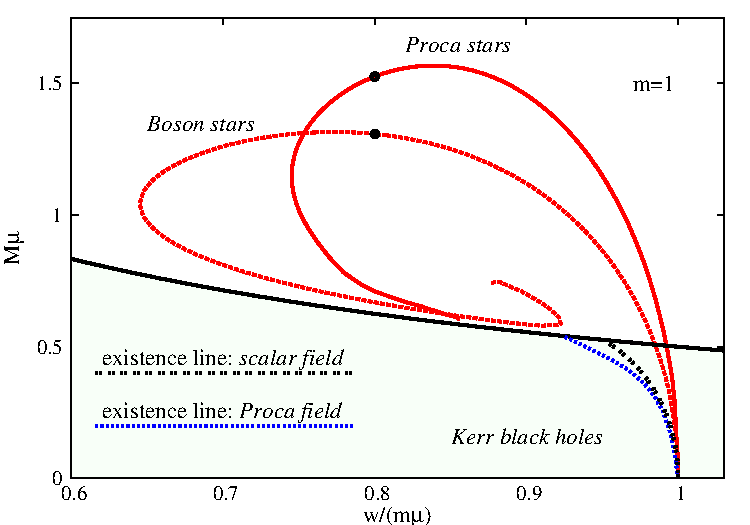
\includegraphics[width=0.7\textwidth]{papers/Proca/wM-m1-comparison.pdf}
  \end{center}
 \caption{Existence line for Proca stationary clouds with $m=1$ (blue dotted line) and the comparable existence line for scalar stationary clouds (with $m=1=\ell$, $n=0$, $cf.$~\cite{Benone:2014ssa}, black double dotted line), in an ADM mass $vs.$ frequency $w/m=\Omega_H$ diagram of Kerr BHs. Both axes are shown in units of the scalar/Proca field mass $\mu$. The black solid line corresponds to extremal Kerr BHs and non-extremal solutions exist below that line. Two red lines describing scalar boson stars (dotted) and Proca stars (solid) are also shown, that will be described in the next section.}
  \label{clouds}
\end{figure}

As can be seen from Fig. \ref{clouds}, there exist Kerr black holes that are superradiantly stable against all $m=1$ scalar perturbations but are superradiantly unstable against $m=1$ Proca modes.
A similar feature has been observed comparing the existence lines for \textit{Maxwell} and scalar stationary clouds in Kerr-AdS~\cite{Wang:2015fgp}.
As we saw in Chapter \ref{ch:Q}, including self-interactions in the scalar field model these stationary clouds can exist in open set of the $(M,\Omega_H)$ space, rather than a one-dimensional line.
We expect this to be the case as well if one would include self-interacting Proca fields, especially in view of the results in~\cite{Loginov:2015rya}.

We close this section by commenting on the node number of these stationary Proca clouds. 
In the scalar case, the number of nodes $n$ of the radial function defining the scalar field profile, 
is $n=0$ for fundamental states and $n\in \mathbb{N}$ for excited states. 
This issue becomes more subtle for Proca clouds (and Proca stars), 
since one has more than one potential component. Nevertheless, we remark that the all states we have obtained so far have always (only)
one node for the temporal component of the Proca potential  $V$, and thus are likely to represent the fundamental
modes of the problem.\footnote{The electric potential of the $m=0$ 
spherically symmetric Proca stars necessarily possesses at least one node \cite{Brito:2015pxa}.
Although the proof there cannot be generalized to the axially symmetric case,
we could not find any numerical indication for the existence of $m\geq 1$ nodeless solutions. 
}

%%%%%%%%%%%%%%%%%%%%%%%%%%%%%%%%%%%%%%%%%%%%%%%%%%%%%%%%%%%%%%%%%%%%%%%%%%%%%%
\section{Spinning Proca stars} 
\label{sec_stars}
%%%%%%%%%%%%%%%%%%%%%%%%%%%%%%%%%%%%%%%%%%%%%%%%%%%%%%%%%%%%%%%%%%%%%%%%%%%%%%
The stationary Proca clouds described in the previous section form one of the central ingredients to understand KBHsPH.
They also form a part of the boundary of the domain of existence of these BHs, as we shall see in the next section. The other central ingredient corresponds to Proca stars, which again will form a part of the boundary of the domain of existence of KBHsPH. We shall now briefly review the relevant properties of these solutions, recently found in~\cite{Brito:2015pxa}, in order to understand KBHsPH better.

Proca stars can be either spherically symmetric and static or axially symmetric and stationary. The former are found by taking a general spherically symmetric ansatz for the line element and an ansatz of the form $\mathcal{A}=e^{-iwt}\left[f(r)dt+ig(r)dr \right]$ for the Proca field.
With this ansatz, however, there are no BH solutions\cite{Herdeiro:2016tmi}. The latter are found by taking a metric ansatz of the form~\eqref{eqn:HBH-ansatz}, with $r_H=0$, with unspecified functions $F_0,F_1,F_2$ and the Proca potential ansatz~\eqref{procaclouds}, with unspecified functions $V,H_2,H_3$.
The remaining two (unspecified) functions are replaced as
\begin{equation}
W\rightarrow \frac{{W}}{r} \ , \qquad H_1\rightarrow \frac{{H_1}}{r} \ . 
\label{ww}
\end{equation}
We find it preferable to work with the new ${W},{H_1}$ when dealing with stars, due to their boundary conditions at the origin (rather than at a horizon). In the remaining of this section we shall always refer to these new functions.
Solving the corresponding field equations with the following boundary conditions:
\begin{description}
\item[i)] at infinity,~\eqref{bccloudslarge}, together with
\begin{equation}
F_i\big|_{r=\infty}={W}\big|_{r=\infty}=0 \ , 
\label{bcstarslarge}
\end{equation}
\item[ii)] on the symmetry axis,~\eqref{bccloudsaxis}, together with 
\begin{equation}
 \partial_\theta F_i\big|_{\theta=0,\pi}=\partial_\theta {W}\big|_{\theta=0,\pi}=0
 \label{bcstarsaxis}
 \end{equation}
 \item[iii)] at the origin, 
 \begin{equation}
 \partial_r F_i\big|_{r=0}={W}\big|_{r=0}=H_i|_{r=0}=V|_{r=0}=0 \ .
 \end{equation}
\end{description} 
 %
 Then, one finds a countable number of families of rotating Proca stars, labelled by $m\in \mathbb{Z}$, of which the cases with $m=1,2,3$ were discussed in~\cite{Brito:2015pxa}.  Therein, it was also found that, as for the scalar rotating boson stars, the ADM angular momentum and the Noether charge obey the simple relation 
 %
 \begin{equation}
 J=mQ \ .
\label{amnc}
 \end{equation}
%
In \cite{Herdeiro:2016tmi}, a detailed derivation and discussion of this relation is given, which is more subtle in the case of Proca stars than for scalar boson stars.
Following~\cite{Herdeiro:2014goa} and the discussion in Chapter \ref{ch:intro}, we define the normalized Noether charge, $q$, as 
 \begin{equation}
 q\equiv \frac{mQ}{J} \ ,
 \label{jq}
 \end{equation}
 which is obviously $q=1$ for all Proca stars, but will be $q\in [0,1]$ for KBHsPH.
 
 For $m=1$, the case in which we focus here, the Proca star solutions 
appear to form a spiral in an ADM mass, $M$, $vs.$ Proca field frequency, $w$, diagram, starting from $M=0$ for $w=\mu$, in which limit the Proca field becomes very diluted and the solution trivializes. 
At some intermediate frequency, a maximal ADM mass is attained. For $m=1$ this frequency is $w_{\rm max}/\mu=0.839$ and the maximal mass is $\mu M_{\rm max}=1.568$, a slightly larger value than for the corresponding scalar rotating boson star (for which $\mu M_{\rm max}=1.315$)~\cite{Brito:2015pxa}. 
This structure is very reminiscent of boson stars.
 
In Fig.~\ref{clouds}, we display the $m=1$ Proca star and scalar boson star curves (red solid and dotted lines). Comparing them, we observe: $(i)$ the slightly larger maximal mass for the Proca stars; $(ii)$ that the backbending of the inspiraling curve occurs for a larger value of the frequency parameter for Proca stars, and hence they exist in a narrower frequency interval; $(iii)$ whereas for scalar boson stars with $m=1$ it was possible to obtain a third branch of solutions (after the second backbending) numerics become very difficult for Proca stars already on the second branch;\footnote{In the spherically symmetric case, 
the results in \cite{Brito:2015pxa} show the existence of a very similar picture for both 
  Proca stars and scalar boson stars, with the occurance  of secondary branches (together with the corresponding
spiral in a $(w,M)$-diagram) also in the former case.} for example, 
the function $F_0$ takes very large, negative values.
Finally, in complete analogy with the scalar boson star case, the Proca star line yields the second boundary of the domain of existence of KBHsPH; the latter reduce to Proca stars when the horizon size vanishes, as will be seen in the next section. 

Although spinning Proca stars are quite similar to spinning scalar boson stars in many aspects, the energy and angular momentum density of the former exhibit novel features with respect to the latter.
Spinning scalar boson stars for generic $m\geqslant 1$ are often described as an effective mass torus in general relativity~\cite{Schunck:1996he}, since surfaces of constant energy density present a toroidal topology sufficiently close to the centre of the star (see $e.g.$ the plots in~\cite{Herdeiro:2014ima}).
Spinning Proca stars, on the other hand, have a different structure for $m=1$ and $m>1$ as shown in Figs.~\ref{PS1}--\ref{3D} for illustrative cases (with $w=0.8$ and along the first branch for all examples).
For $m=1$, the Proca star's energy density has a maximum at the origin and a second maximum (smaller) at some radial distance, thus presenting a composite-like structure, $cf.$ Fig.~\ref{PS1} (top left panel): instead of being toroidal, constant energy surfaces are \textit{Saturn-like} - Fig.~\ref{3D} (left panel).
The angular momentum density, on the other hand, is zero at the origin and has two local positive maxima at some radii and one local negative minimum between them -- Fig.~\ref{PS1} (top right panel); interestingly this means there is a counter-rotating toroidal-like region.
For $m>1$ the Proca star's energy density vanishes at the origin and two local maxima arise at different radial values, $cf.$ Fig.~\ref{PS2} (top left panel).
Thus some constant energy density surfaces are \textit{di-ring-like} - Fig.~\ref{3D} (right panel).
The angular momentum density is similar to the $m=1$ case -- Fig.~\ref{PS2} (top right panel).


\begin{figure}[h!]
  \begin{center}
    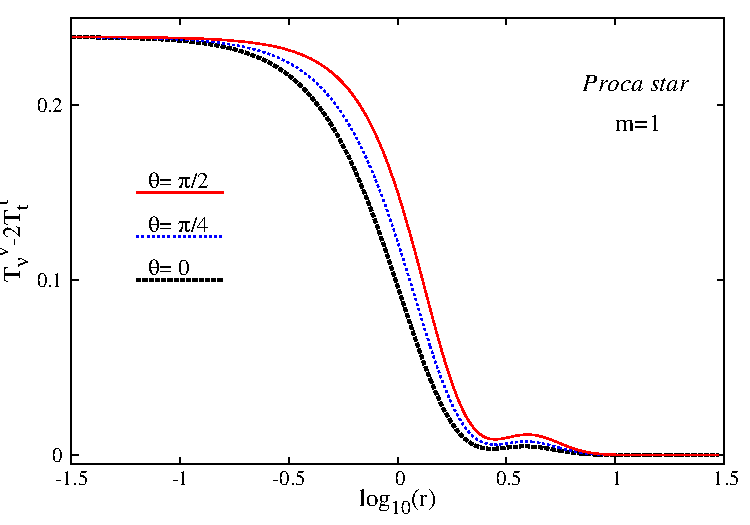
\includegraphics[width=8.1cm]{papers/Proca/PS-ro-m1.pdf}
    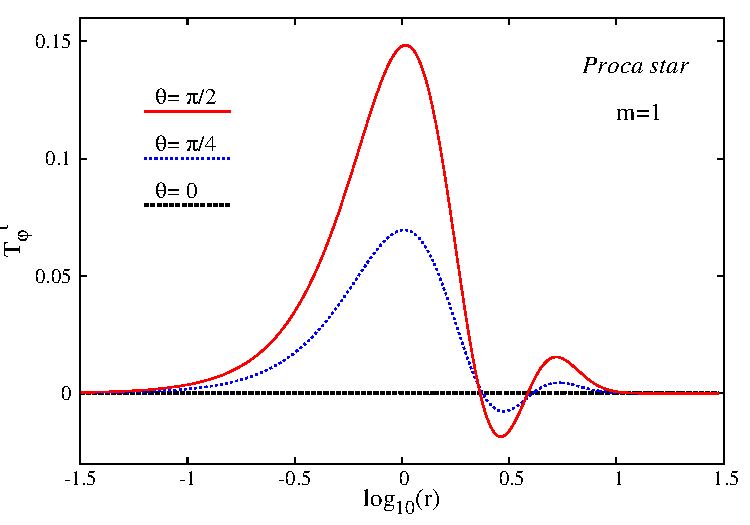
\includegraphics[width=8.1cm]{papers/Proca/PS-T34-m1.pdf}   
    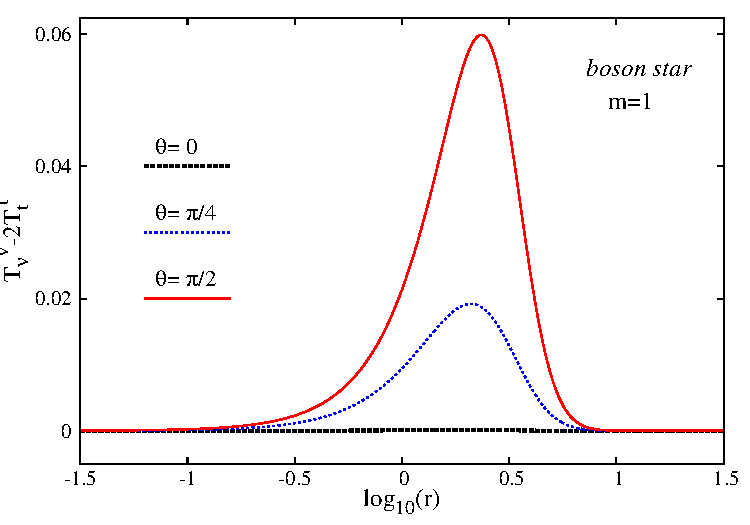
\includegraphics[width=8.1cm]{papers/Proca/BS-ro-m1.pdf}
    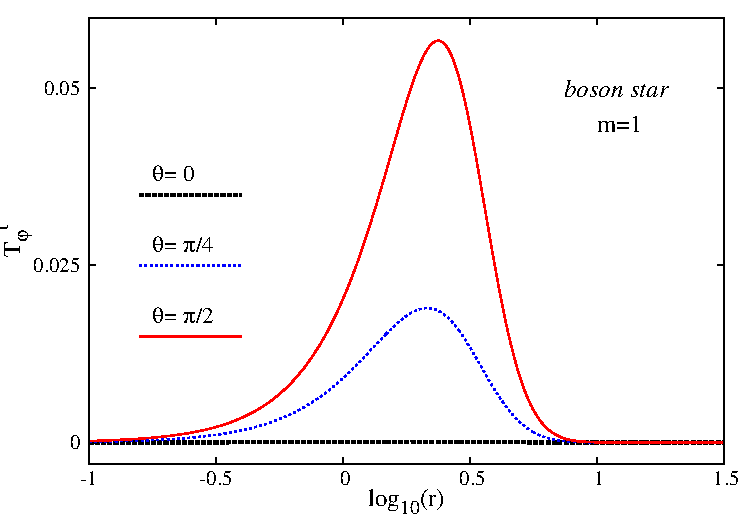
\includegraphics[width=8.1cm]{papers/Proca/BS-T34-m1.pdf}
  \end{center}
 \caption{Radial variation of the energy density, $cf.$~\eqref{ed} (left panel), and angular momentum density, $cf.$~\eqref{amd}  (right panel),  of the Proca field, for different constant $\theta$ sections of a spinning Proca star with $m=1$ (top panels) and a spinning scalar boson star with $m=1$ (bottom panels). Both solutions have $w=0.8$ and are marked with a bullet in Fig.~\ref{clouds}. The Proca star has $\mu M= 1.526$,  $\mu^2J= 1.575$, while the scalar boson star has $\mu M=1.308$, $\mu^2J=1.372$.}
  \label{PS1}
\end{figure}



\begin{figure}[h!]
  \begin{center}
    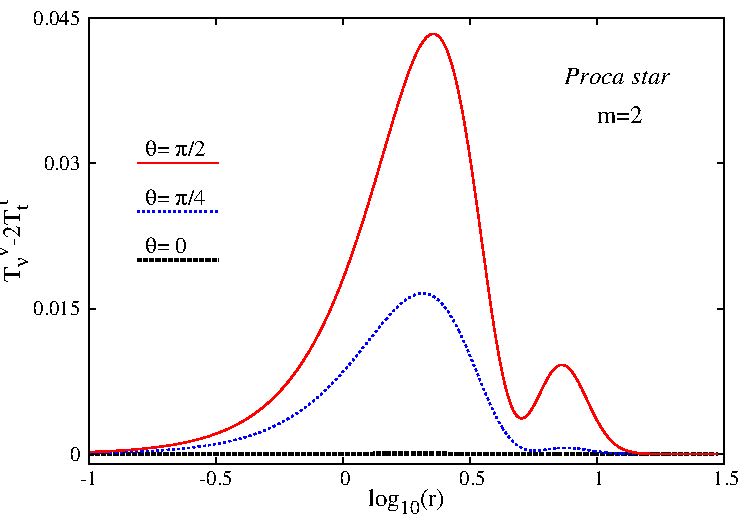
\includegraphics[width=8.1cm]{papers/Proca/PS-ro-m2.pdf}
    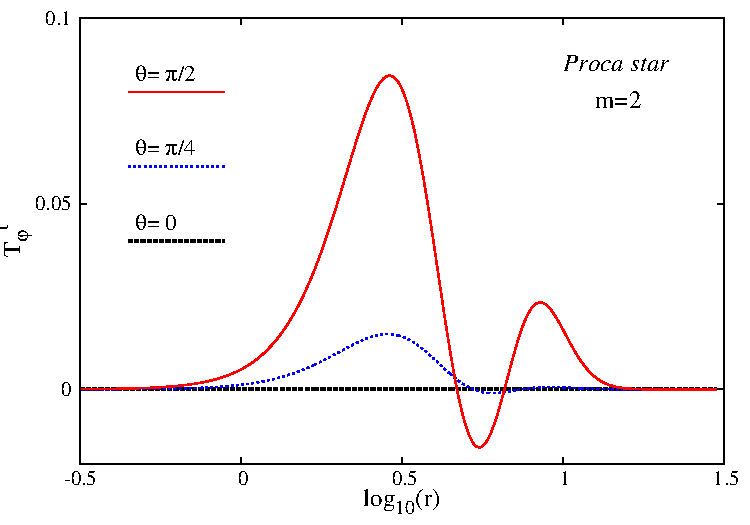
\includegraphics[width=8.1cm]{papers/Proca/PS-T34-m2.pdf}   
    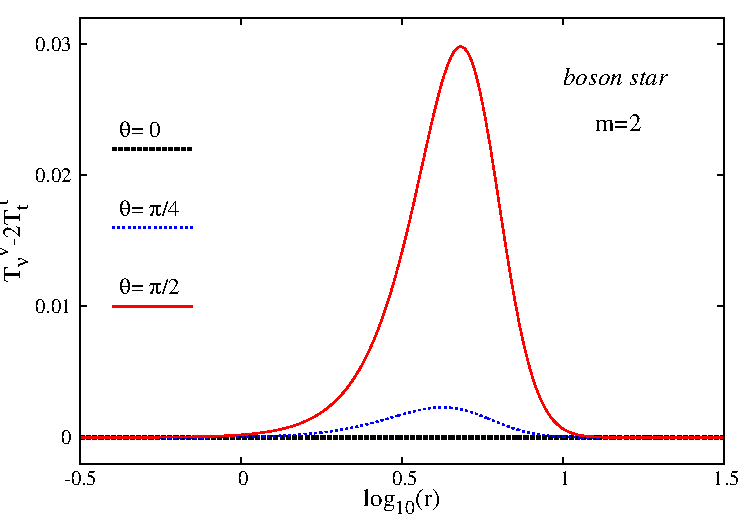
\includegraphics[width=8.1cm]{papers/Proca/BS-ro-m2.pdf}
    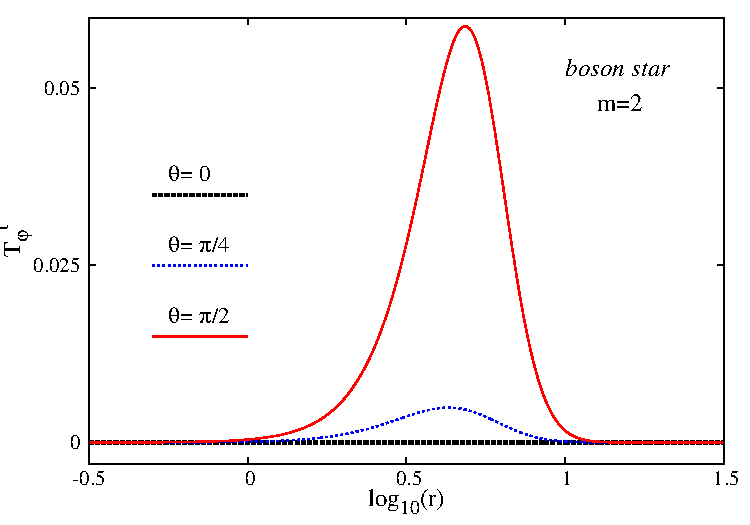
\includegraphics[width=8.1cm]{papers/Proca/BS-T34-m2.pdf}
  \end{center}
 \caption{Same as in Fig.~\ref{PS1} but for $m=2$. Both solutions have $w=0.8$. The Proca star has $\mu M=2.319$, 
$\mu^2J=4.873$ whereas the scalar boson star has $\mu M=2.016$, $\mu^2J=4.272$.}
  \label{PS2}
\end{figure}


\begin{figure}[h!]
  \begin{center}
    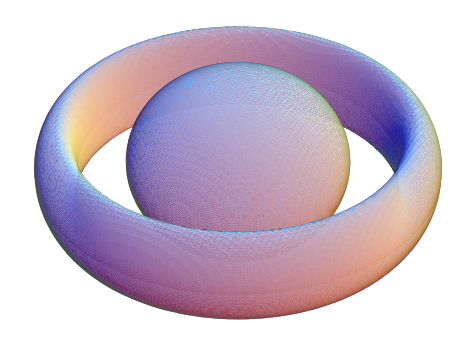
\includegraphics[width=6.1cm]{papers/Proca/3DPS1-m=1-v2.pdf} \qquad \qquad 
    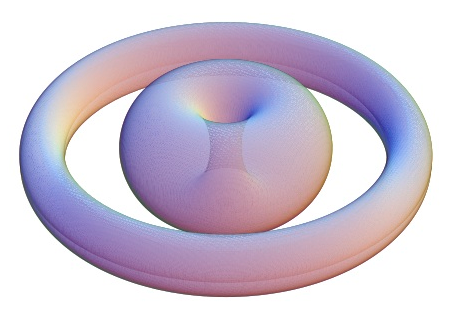
\includegraphics[width=6.1cm]{papers/Proca/3DPS1-m=2-v2.pdf}   
         \end{center}
 \caption{Left (right) panel: Saturn-like (di-ring-like) surfaces of constant energy density for the $m=1$ ($m=2$) Proca star exhibited in Fig.~\ref{PS1} (Fig.~\ref{PS2}). The corresponding energy density is $0.011$ ($0.008$). We emphasize these are not embedding diagrams; rather we defined Cartesian coordinates regarding the $r,\theta,\varphi$ coordinate system used here as standard spherical coordinates.}
  \label{3D}
\end{figure}

Finally, we discuss how ``compact'' these Proca stars are.
Proca stars, like their scalar cousins, have no surface, $i.e.$ the Proca field decays exponentially towards infinity.
Thus, there is no unique definition of the Proca star's ``radius''.
To obtain an estimate we follow the discussion in~\cite{AmaroSeoane:2010qx,Herdeiro:2015gia}.
Using the ``perimeteral'' radius, $i.e.$ a radial coordinate $R$ such that a circumference along the equatorial plane has perimeter $\simeq 2\pi R$,  we compute $R_{99}$, the perimeteral radius containing 99\% of the Proca star mass, $M_{99}$. Then, we define the inverse compactness by comparing $R_{99}$ with the Schwarzschild radius associated to 99\% of the Proca star's mass, $R_{Schw}=2M_{99}$:
%
\begin{equation}
{\rm Compactness}^{-1}\equiv  \frac{R_{99}}{2M_{99}} \ .
\label{compactness}
\end{equation}
%
The result for the inverse compactness of Proca stars with $m=1$ is exhibited in Figure~\ref{compactnessfig}.
With this measure, the inverse compactness is always greater than unity; $i.e.$, Proca stars are less compact than BHs, as one would expect, but, as can be seen from the figure, they are also less compact than comparable scalar boson stars.

\begin{figure}[h!]
  \begin{center}
    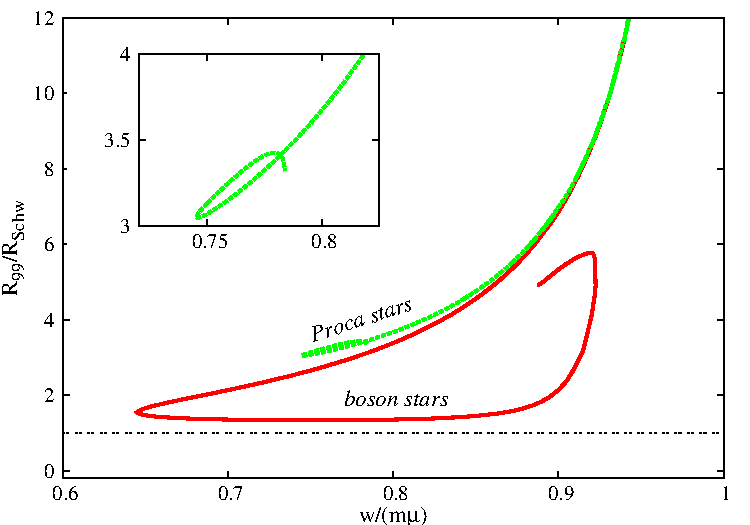
\includegraphics[width=0.7\textwidth]{papers/Proca/w-Comp-Schw.pdf}  
         \end{center}
 \caption{Inverse compactness of Proca stars compared to that of the scalar boson stars with $m=1$, defined in~\eqref{compactness}. The inset shows a detail of the Proca stars curve.}
  \label{compactnessfig}
\end{figure}

%%%%%%%%%%%%%%%%%%%%%%%%%%%%%%%%%%%%%%%%%%%%%%%%%%%%%%%%%%%%%%%%%%%%%%%%%%%%%%
\section{Kerr BHs with Proca Hair} 
\label{sec_kbhsph}
%%%%%%%%%%%%%%%%%%%%%%%%%%%%%%%%%%%%%%%%%%%%%%%%%%%%%%%%%%%%%%%%%%%%%%%%%%%%%%

We are now prepared to take on KBHsPH.
The parallelism with the scalar case for both the stationary clouds and the solitonic limit is striking and one anticipates a high degree of similarity also at the level of the hairy BH solutions. 

The metric ansatz for constructing KBHsPH is the same as for the previous examples of hairy black holes, i.e. Eq.~\eqref{eqn:HBH-ansatz}, where now all four (unspecified) functions $F_0,F_1,F_2,W$ depend on $(r,\theta)$ and, again, $r_H$ is a constant.
If $F_2$ is finite, then $r={\rm constant}$ surfaces are timelike for $r>r_H$ and become null for $r=r_H$.
Thus, $r=r_H$ is the location of the event horizon if the metric is regular therein.

For $r_H=0$, this ansatz reduces to the one discussed in the previous section for Proca stars, except for the replacement given by Eq.~\eqref{ww}.
The line element form used for Proca stars is useful to tackle the behaviour at the origin, whereas the one used for BHs is useful to tackle the behaviour on a rotating horizon wherein $W$ reduces to the horizon angular velocity, $\Omega_H$.
Indeed, following null geodesic generators, $ds^2=0$ on the horizon, assuming $F_2$ is finite there, implies $d\varphi=W(r_H)dt$ and thus $W(r_H)=\Omega_H$, the angular velocity as measured by the observer at infinity.

The Proca field ansatz is the same as for the stationary Proca clouds (and Proca stars up to the replacements given by Eq.~\eqref{ww}), given by Eq.~\eqref{procaclouds}.
This, again, introduces two parameters: $w>0$, $m\in \mathbb{Z}$.
As for Proca stars we shall focus here on $m=1$, and take the sychronization condition~\eqref{synchronization} that we can rewrite in this context as (for general $m$)
\begin{equation}
\frac{w}{m}=W(r_H) =\Omega_H\ . 
\label{synchronization2}
\end{equation}
This condition was deduced in the context of a test field on the Kerr background and can be related to the threshold of superradiance.
But there is another reason for its presence.
In Appendix~\ref{appendixb}, we present the Einstein tensor and the Proca energy-momentum tensor associated to the ansatz discussed in this section.
A careful inspection of the components of the energy-momentum tensor that have inverse powers of $N$,\footnote{A similar analysis can be made at the level of the components in an orthonormal frame, with similar conclusions.} and hence may diverge at the horizon, shows that, taking into account Eq.~\eqref{bccloudshorizon}, finiteness of the energy-momentum tensor components presented at $r=r_H$ \textit{requires}
\begin{equation}
\frac{w-mW(r_H)}{N(r_H)} 
\end{equation}
to be finite there and hence it requires Eq.~\eqref{synchronization2} to be fulfilled.
The same can be observed in the Einstein equations for KBHsSH, presented in~\cite{Herdeiro:2015gia}.

The Einstein-Proca equations are solved with the following boundary conditions:
\begin{description}
\item[i)] at infinity, the same as for Proca stars,~\eqref{bccloudslarge} and~\eqref{bcstarslarge};
\item[ii)] on the symmetry axis, the same as for Proca stars,~\eqref{bccloudsaxis} and~\eqref{bcstarsaxis};
 
\item[iii)] at the horizon, using again the new radial coordinate $x=\sqrt{r^2-r_H^2}$, a power series expansion near $x=0$ implies~\eqref{bccloudshorizon}, together with
\begin{equation}
\partial_x F_i\big|_{x=0}=0 \ , \qquad W\big|_{x=0}=\Omega_H \ .
\end{equation}
\end{description}
 % 

The Einstein-Proca equations,shown in Appendix \ref{appendixb}), are solved numerically subject to these boundary conditions.


%%%%%%%%%%%%%%%%%%%%%%%%%%%%%%%%%%%%%%%%%%%%%%%%%%%%%%%%%%%%%%%%%%%%%%%%%%%%%%%
\subsection{Physical Quantities}
\label{subsec_II}
%%%%%%%%%%%%%%%%%%%%%%%%%%%%%%%%%%%%%%%%%%%%%%%%%%%%%%%%%%%%%%%%%%%%%%%%%%%%%%% 
In the following we shall describe some physical quantities that will be obtained from the numerical solutions we have found.
The ADM mass, $M$, and ADM angular momentum, $J$, are read off from the asymptotic expansion of the appropriate metric components:
%
\begin{equation}
\label{Pasym}
g_{tt} =-1+\frac{2M}{r}+\dots \ ,\qquad ~~g_{\varphi t}=-\frac{2J}{r}\sin^2\theta+\dots \ . \ \ \ 
\end{equation}
%
We also compute the horizon mass and angular momentum by using the appropriate Komar integrals associated to the corresponding Killing vector fields ${\bf k}$ and ${\bf m}$:
\begin{equation}
M_H=-\frac{1}{8\pi}\oint_{\mathcal{H}}dS_{ab}D^a k^b \ , \qquad 
J_H=\frac{1}{16\pi}\oint_{\mathcal{H}}dS_{ab}D^a m^b \ .
\end{equation}
%
The asymptotic quantities, $M$ and $J$, can also be computed as Komar integrals at infinity.
Then, applying Gauss's law, one obtains a relation with $M_H$ and $J_H$ together with volume integrals on a spacelike surface with a boundary at the (spatial section of the) horizon.
By making use of the Killing identity and the Einstein equations one obtains:
\begin{equation}
M=M_H-2\int_{\Sigma}dS_{a}\left(T^a_b k^b-\frac{1}{2}Tk^a\right) \equiv M_H+M^{(\mathcal{P})}
\end{equation}
This defines the energy stored in the Proca field (outside the horizon):
\begin{equation}
M^{({\cal P})}\equiv - \int_{\Sigma} dr d\theta d\varphi(2T_t^t-T_a^a) \sqrt{-g} \ .
\label{ed}
\end{equation}
%
Proceeding similarly for the angular momentum one obtains:
\begin{equation}
J=J_H+J^{(\mathcal{P})} \ , \ \qquad  J^{({\cal P})}\equiv  \int_{\Sigma} dr d\theta d\varphi T^t_\varphi \sqrt{-g} \ ,
\label{amd}
\end{equation}
which defines the angular momentum stored in the Proca field.
For KBHsSH the angular momentum stored in the scalar field relates to the Noether charge in precisely the same way as for rotating scalar boson stars $J^{(\Psi)}=mQ$, for KBHsPH the relation between $J^{(\mathcal{P})} $ and  the Noether charge~\eqref{Pq} includes an extra boundary term
\begin{equation}
\label{nr1}
J^{(\mathcal{P})}=mQ+ \oint_\mathcal{H}  ({\mathcal{A}}_\varphi \bar{ {\mathcal{F}}}^{r t}+\bar{\mathcal{A}}_\varphi { {\mathcal{F}}}^{r t}  ) dS_r \ ,
\end{equation}
which generalizes relation~\eqref{amnc} to the case of hairy BHs. 
A similar relation can be written for $M^{({\cal P})}$
\begin{equation}
\label{nr2}
M^{({\cal P})}=2w Q
-\mu^2  {\cal U}
+ \oint_\mathcal{H}  
\left[
\frac{1}{2} 
\left(
{\mathcal{A}}_b \bar{ {\mathcal{F}}}^{r b}+\bar{\mathcal{A}}_b { {\mathcal{F}}}^{r b}
\right)
-\left({\mathcal{A}}_t \bar{ {\mathcal{F}}}^{r t}+\bar{\mathcal{A}}_t { {\mathcal{F}}}^{r t}
\right)  
\right] dS_r \ ,
\end{equation}
with
\begin{equation}
\label{ProcaU}
{\cal U}\equiv \int _\Sigma  dr d\theta d\varphi  {\mathcal{A}}_a \bar {\mathcal{A}}^a \sqrt{-g}\ .
\end{equation}


The horizon temperature and event horizon area of the KBHsPH solutions are computed by standard relations, that specialize to: 
\begin{eqnarray}
\label{PTHAH}
T_H=\frac{1}{4\pi r_H}e^{(F_0-F_1)|_{r=r_H}} \ , \qquad
 A_H=2\pi r_H^2 \int_0^\pi d\theta \sin \theta  e^{(F_1+F_2)|_{r=r_H}}\ . 
 \end{eqnarray}
Then, the ADM quantities $M,J$ are related to $T_H,S,Q,M^{({\cal P})}$, where $S=A_H/4$ is the horizon entropy, through a Smarr formula  
%
\begin{eqnarray}
\label{Psmarr} 
M=2 T_H S +2\Omega_H J_H+ M^{({\cal P})} \ .
\end{eqnarray}
The variation of $M$ can be expressed by the first law
\begin{equation}
\label{fl}
dM=T_H dS +\Omega_H dJ \ .
\end{equation}
We note that
by making use of relations
(\ref{nr1})
and
(\ref{nr2}),
 the Smarr formula (\ref{Psmarr})
can be written in a Kerr-like form
\begin{eqnarray}
\label{smarr-new1} 
M=2 T_H S +2\Omega_H J-\mu^2 {\cal U} \ ,
\end{eqnarray}
which renders explicit the fact that the solutions are supported by
a nonzero mass term of the Proca field, as is evident from the last term in the equation.

%%%%%%%%%%%%%%%%%%%%%%%%%%%%%%%%%%%%%%%%%%%%%%%%%%%%%%%%%%%%%%%%%%%%%%%%%%%%%%%
\subsection{The domain of existence and phase space}
\label{subsec_III}
%%%%%%%%%%%%%%%%%%%%%%%%%%%%%%%%%%%%%%%%%%%%%%%%%%%%%%%%%%%%%%%%%%%%%%%%%%%%%%% 
We have scanned the domain of existence of KBHsPH by varying $r_H$ for fixed $w$ lines, 
in between the minimum frequency 
$w_{\rm min}/\mu=0.7453$ and the maximal one $w=\mu$. 
The result for the $m=1$ family of KBHsPH is shown in Fig.~\ref{figdomain} obtained from over five thousand numerical points. 


%
\begin{figure}[h!]
  \begin{center}
    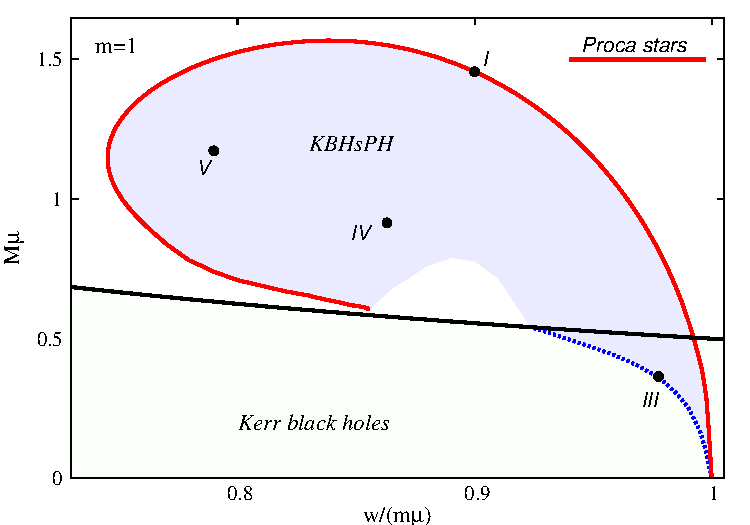
\includegraphics[width=0.7\textwidth]{papers/Proca/BH-w-M-with-points.pdf}
      % 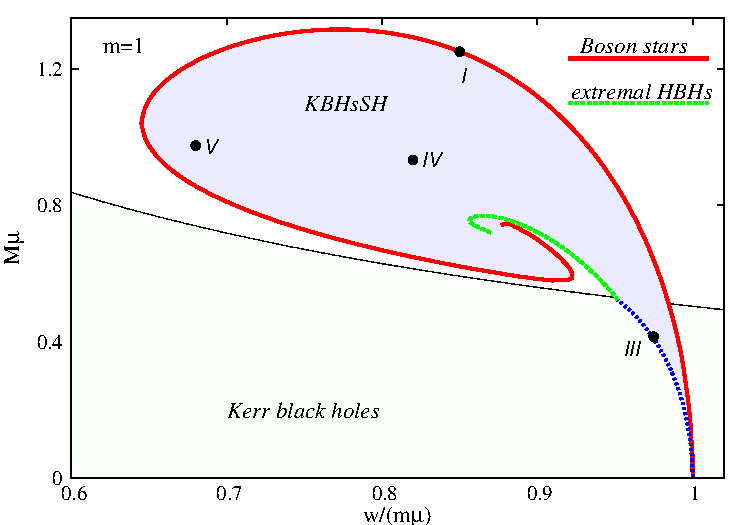
\includegraphics[width=8.1cm]{papers/Proca/scalar-BH-w-M.pdf}
  \end{center}
  \caption{ADM mass $vs.$ frequency $w$ diagram for $m=1$ KBHsPH. The red solid lines correspond to the solitonic limit. The blue dotted lines are the Kerr limit, also shown in Fig.~\ref{clouds}. Kerr solutions exist below the black solid line, which corresponds to extremal Kerr solutions. The hairy BHs exist in the blue shaded region. Points I,III,IV,V, in each case, correspond to specific solutions for which the numerical data is publicly available~\cite{datakbhph,datakbhsh}. The right panel also shows the extremal hairy BHs (green dashed) line.}
  \label{figdomain}
\end{figure}
%

Just as for KBHsSH, the domain of existence of KBHsPH should be bounded by three lines: the Proca clouds existence line discussed in Section~\ref{sec_clouds}, the Proca star line discussed in Section~\ref{sec_stars} and the line of extremal KBHsPH ($i.e.$ zero temperature).
So far, the last of the three was only obtained by extrapolating to $T_H=0$ the non-extremal solutions, as our attempts to construct the extremal KBHsPH solutions by directly solving the Einstein-Proca field equations were unsuccessful (unlike the scalar case, as reported in~\cite{Herdeiro:2015gia} and Chapter \ref{ch:SI} for self-interacting solutions).
For this reason we have chosen not to display this line in Fig.~\ref{figdomain}, for the Proca case.
Another technical difficulty arises in trying to connect the set of (extrapolated) extremal solutions with the set of Proca stars.
As for the case of KBHsSH, these two curves are likely to meet in a critical point at the center of the 
Proca stars spiral; however, validation of this hypothesis is a numerical challenge, both for the Proca and scalar case.

In Fig.~\ref{figdomain} we have singled out four particular solutions for each case, denoted I,III,IV and V. The numerical data for these four solutions, together with the data for a vacuum Kerr solution with the same ADM mass and angular momentum as that of configuration III, for each case, has been made publicly available for community use~\cite{datakbhph,datakbhsh}.
The corresponding parameters are detailed in Appendix~\ref{appendixd} along with similar data for KBHsSH.

In Fig.~\ref{fig2} we exhibit the phase space, $i.e.$ ADM mass $vs.$ ADM angular momentum diagram for $m=1$ solutions of KBHsPH.
The plot is quite similar to the top left panel of Fig.~\ref{fig:no-HBHs} and the features we wish to emphasize is that, as for the scalar case, one observes violation of the Kerr bound (in terms of ADM quantities) and non-uniqueness, $i.e$ there are both hairy and vacuum Kerr BHs with the same ADM mass and angular momentum ($cf.$ Appendix~\ref{appendixd}). 


\begin{figure}[h!]
  \begin{center}
    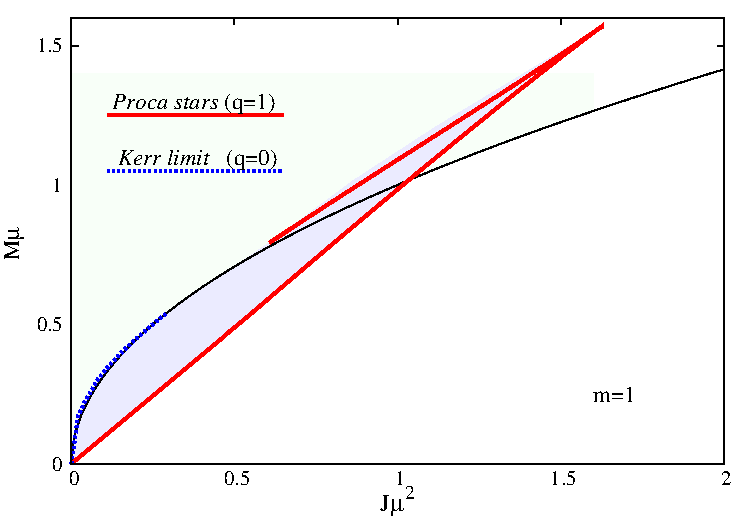
\includegraphics[width=0.7\textwidth]{papers/Proca/BH-J-M.pdf}
  \end{center}
  \caption{ADM mass $vs.$ ADM angular momentum diagram for $m=1$ KBHsPH, in units of the field mass. The black solid line corresponds to extremal Kerr solutions; non extremal BHs exist above this line. The red solid line is for Proca stars in the left panel. The blued dotted line is the existence line, denoting Kerr BHs that support Proca clouds. The blue shaded region is the domain of existence of KBHsPH.}
  \label{fig2}
\end{figure}
 

The violation of the Kerr bound also occurs in terms of \textit{horizon} quantities, as shown in Fig.~\ref{vconjecture} (right panel). For these solutions the conjecture put forward in~\cite{Herdeiro:2015moa} concerning the horizon linear velocity $v_H$, as defined therein, holds: despite violating the Kerr bound both in terms of ADM and horizon quantities, $v_H$ never exceeds the speed of light.
We recall $v_H$ is defined as follows: for asymptotically flat, stationary and axi-symmetric spacetimes, on a spatial section of the event horizon one computes the proper length of all closed orbits of ${\bf m}$.
If $L_{\rm max}$ is the maximum of all such proper lengths; the corresponding circumferencial radius is $R_c\equiv {L_{\rm max}}/({2\pi})$. 
Then the horizon linear velocity is $v_H \equiv R_c \Omega_H$ \cite{Herdeiro:2015moa}.

\begin{figure}[h!]
  \begin{center}
    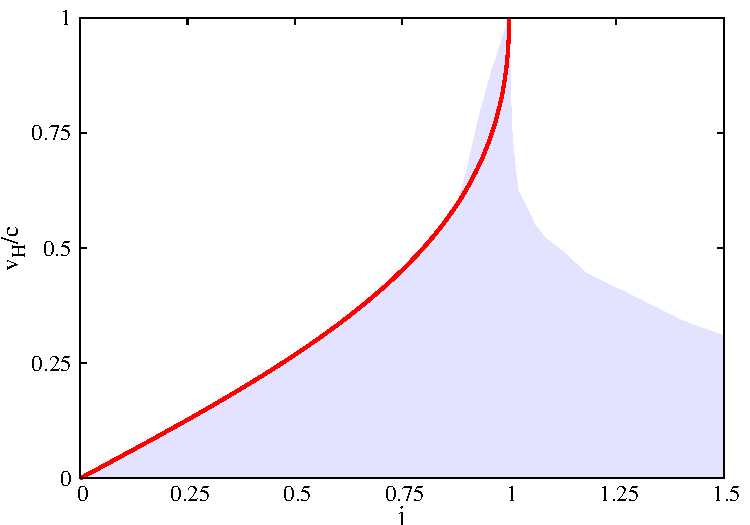
\includegraphics[width=8.1cm]{papers/Proca/ProcaBH-j-v-bound.pdf}
      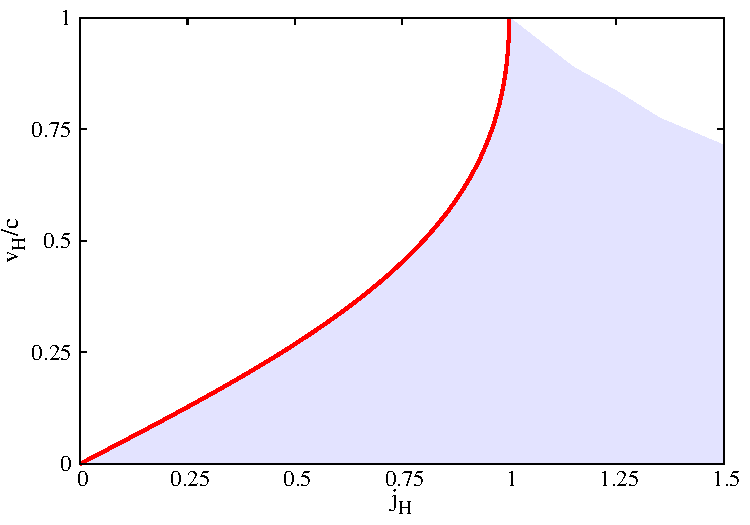
\includegraphics[width=8.1cm]{papers/Proca/ProcaBH-jKv-bound.pdf}
  \end{center}
 \caption{Linear velocity of the horizon normalized to the speed of light, $v_H$, versus:  (left panel)  the ADM dimensionless spin parameter $j\equiv Jc/GM^2$, where $M,J$ are the ADM mass and angular momentum; (right panel) the horizon dimensionless spin parameter $j_H\equiv J_Hc/GM_H^2$, where $M_H,J_H$ are the horizon mass and angular momentum. Here we have reinstated $c,G$. The red solid line corresponds to vacuum Kerr and the shaded area is filled by KBHsPH.}
  \label{vconjecture}
\end{figure}

%%%%%%%%%%%%%%%%%%%%%%%%%%%%%%%%%%%%%%%%%%%%%%%%%%%%%%%%%%%%%%%%%%%%%%%%%%%%%%%
\subsection{Energy distribution and horizon quantities}
\label{subsec_IV}
%%%%%%%%%%%%%%%%%%%%%%%%%%%%%%%%%%%%%%%%%%%%%%%%%%%%%%%%%%%%%%%%%%%%%%%%%%%%%%%
As for their scalar counterparts, KBHsPH can be thought of as a bound state of a horizon with a Proca star.
Thus, the matter energy density distribution around the horizon will resemble that of (some) Proca stars.
In~Fig.~\ref{figenergybhs} we exhibit the energy density and the angular momentum density as a function of the radial coordinate for different angular sections for an example of KBHPH.
As for the Proca stars, both the energy density and the angular momentum density can have more than one maximum outside the horizon and the latter can also have regions with a different sign.
Thus, outside KBHsPH there are counter-rotating regions.
In Fig.~\ref{fig3Dbh} a constant Proca energy density surface is exhbited in a 3D plot.
The behaviour of the energy density and angular momentum density on the horizon is more clearly seen in Fig.~\ref{horizoned}.


\begin{figure}[h!]
  \begin{center}
    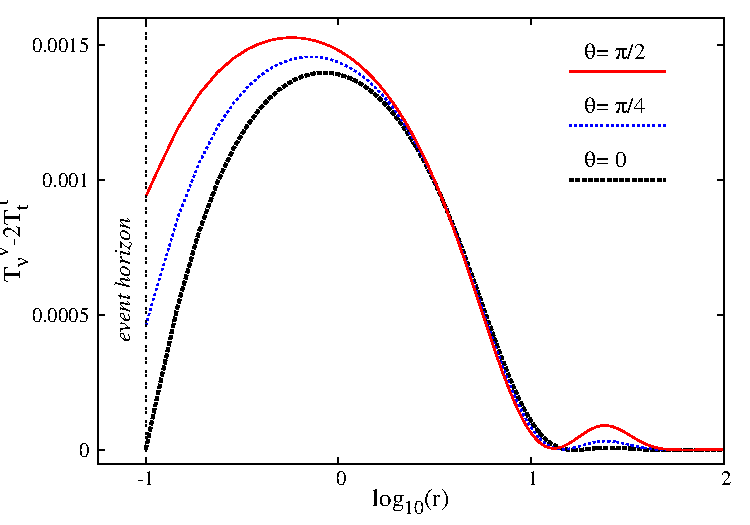
\includegraphics[width=8.1cm]{papers/Proca/BH-ro-m1.pdf}
      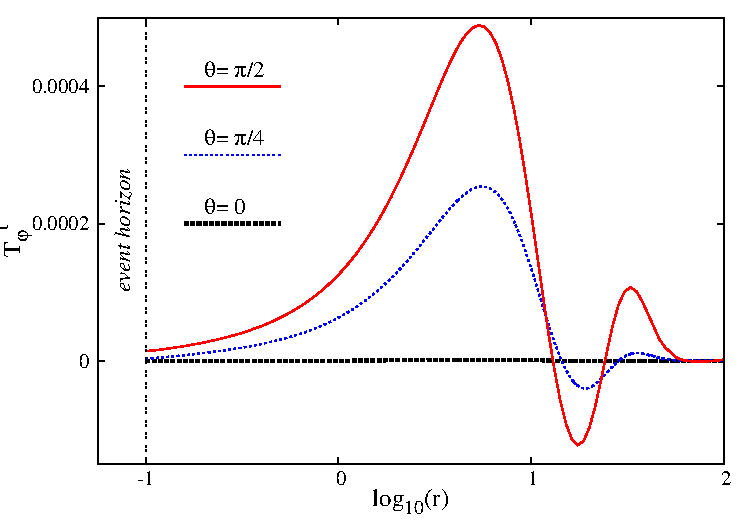
\includegraphics[width=8.1cm]{papers/Proca/BH-T34.pdf}
  \end{center}
  \caption{Radial variation of the energy density, $cf.$~\eqref{ed} (left panel), and angular momentum density, $cf.$~\eqref{amd}  (right panel),  of the Proca field, for different constant $\theta$ sections of a KBHPH with $m=1$, $w=0.98\mu$, $r_H=0.1$,  $\mu M=0.701$ and $\mu^2J=0.652$.}
  \label{figenergybhs}
\end{figure}



\begin{figure}[h!]
  \begin{center}
    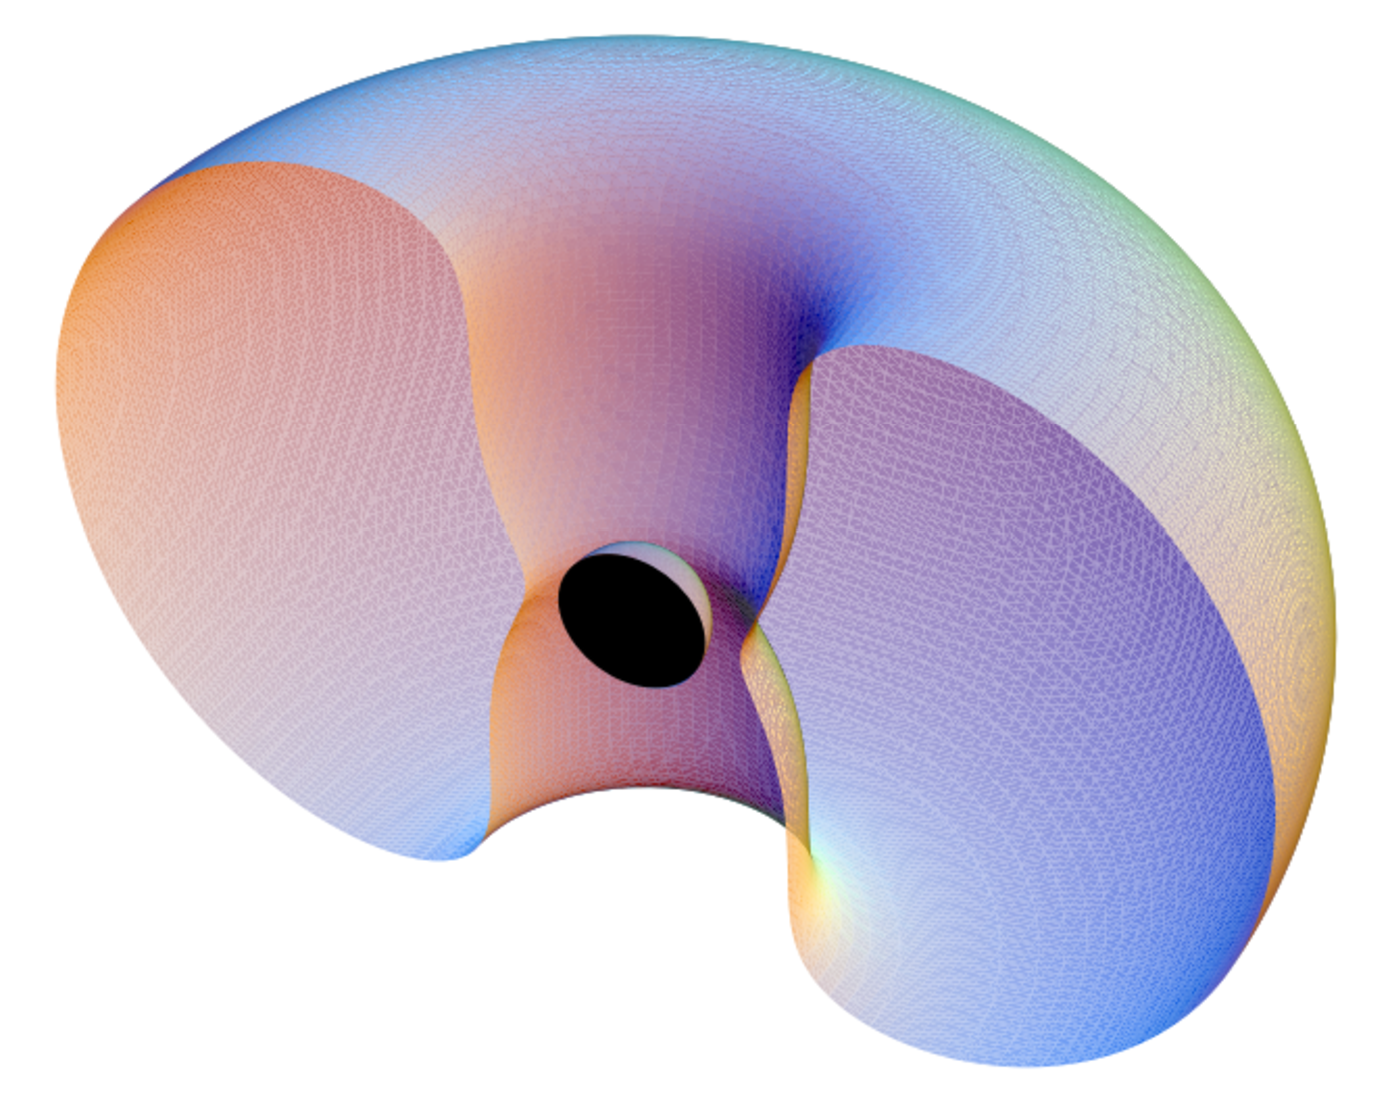
\includegraphics[width=6.1cm]{papers/Proca/3Dbh.pdf}
  \end{center}
  \caption{One toroidal-like surface of constant energy density (corresponding to $0.00142$) for the same KBHPH displayed in Fig.~\ref{figenergybhs}. We also plot the spatial section of the event horizon in these coordinates (half-sphere with the black cross section).}
  \label{fig3Dbh}
\end{figure}


\begin{figure}[h!]
  \begin{center}
    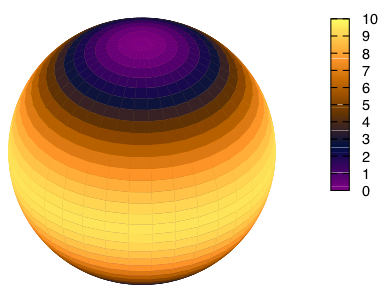
\includegraphics[width=5.5cm]{papers/Proca/Ttr-horizon.pdf}\qquad \qquad 
      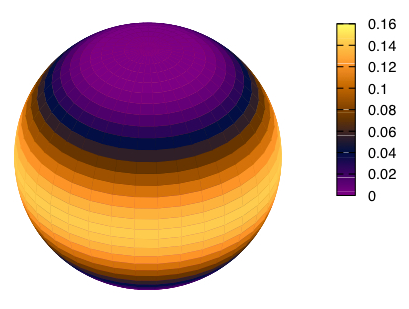
\includegraphics[width=6.0cm]{papers/Proca/T34-horizon.pdf}
  \end{center}
  \caption{Energy density, $cf.$~\eqref{ed} (left panel), and angular momentum density, $cf.$~\eqref{amd}  (right panel),  of the Proca field on the horizon for the same example of a KBHPH displayed in Fig.~\ref{figenergybhs}. The corresponding values were multiplied by $10^4$ for better visualization.}
  \label{horizoned}
\end{figure}


Finally, in Fig.~\ref{temperature} we exhibit the variation of the horizon area with the horizon temperature along sequences of solutions with constant horizon angular velocity (or frequency).
For both KBHsPH (left panel) and KBHsSH (right panel) one can see three different types of behaviour, which are easy to interpret referring back to Fig.~\ref{figdomain}.
For large values of $\Omega_H$, the solutions interpolate between the Kerr existence line and the corresponding (Proca or scalar boson) star line (for which $T_H\rightarrow \infty$).
For intermediate values of $\Omega_H$, the solutions interpolate between the extremal BHs line (for which $T_H\rightarrow 0$) and the corresponding star line.
Finally, for sufficiently small values of $\Omega_H$, the solutions interpolate between two stars, and thus start and end for $T_H\rightarrow \infty$.


\begin{figure}[h!]
  \begin{center}
    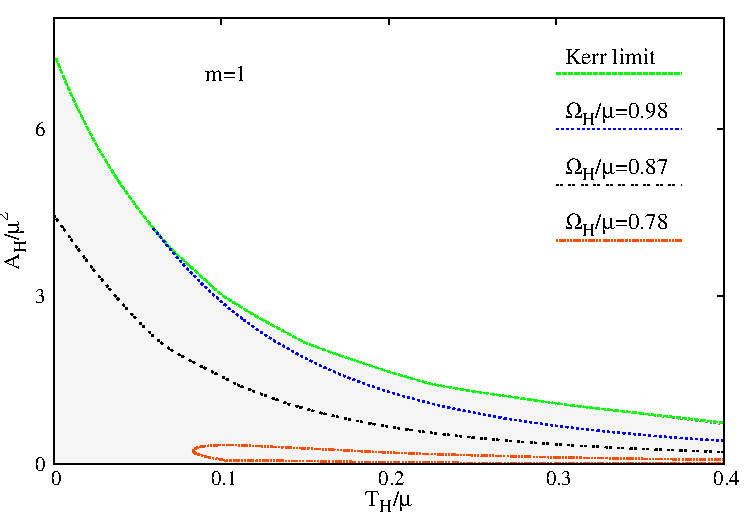
\includegraphics[width=8.1cm]{papers/Proca/BH-TH-AH.pdf}
      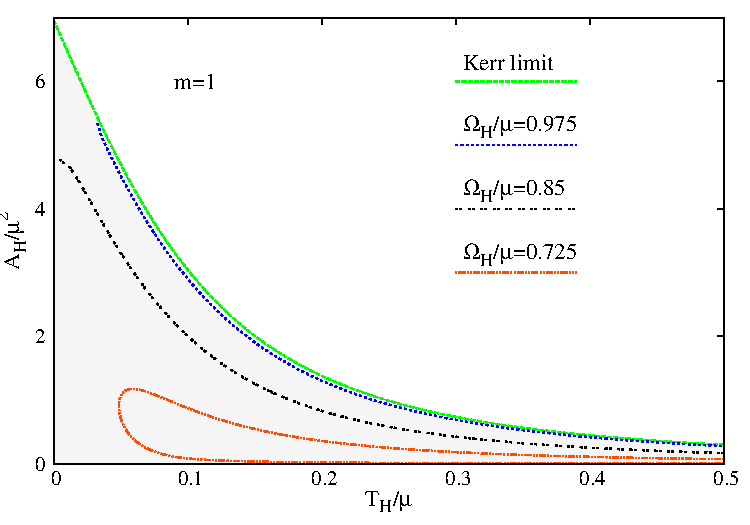
\includegraphics[width=8.1cm]{papers/Proca/scalar-BH-TH-AH.pdf}
  \end{center}
 \caption{Event horizon area $vs.$ temperature for KBHsPH (left panel) and KBHsSH (right panel), in units of $\mu$, for different constant angular velocity sets of solutions.}
  \label{temperature}
\end{figure}
%%%%%%%%%%%%%%%%%%%%%%%%%%%%%%%%%%%%%%%%%%%%%%%%%%%%%%%%%%%%%%%%%%%%%%%%%
\section{Discussion}
\label{sec_discussion}
%%%%%%%%%%%%%%%%%%%%%%%%%%%%%%%%%%%%%%%%%%%%%%%%%%%%%%%%%%%%%%%%%%%%%%%%%%%%%%%
It has long been established that stationary, asymptotically flat BHs in Einstein's gravity minimally coupled to one or many real, Abelian Proca fields cannot have Proca hair.
The basic theorem supporting this idea, due to Bekenstein~\cite{Bekenstein:1971hc,Bekenstein:1972ky}, assumes, however, that the Proca field inherits the spacetime isometries.
In this chapter we have shown that dropping this assumption Kerr BHs with Proca hair exist under two conditions:
\begin{description}
\item[i)] The Proca field is complex, or equivalently there are two real Proca fields with the same mass. These solutions can be, moreover, generalized to an arbitrary number of complex Proca fields (any even number of real Proca fields), without mutual interactions, and all of them minimally coupled to gravity. Here, however, we focus on a model with a single complex Proca field. 
\item[ii)] The complex Proca field has a harmonic time dependence, as in the ansatz~\eqref{procaclouds}, with the frequency and azimuthal harmonic index obeying the synchronization condition~\eqref{synchronization}.
\end{description}
These two assumptions, together, allow the two real Proca fields to oscillate, with the same frequency but opposite phases, hence cancelling out gravitational radiation emission (as well as Proca radiation emission).
It remains as an open question if the same could be achieved with a single real Proca field, especially in view of the result in~\cite{Wang:2015fgp}, since such real Proca field already has two independent modes. 

\bigskip

In the next chapter, we move back to the scalar hair case but now we will consider both a charged black hole and a charged field.
That is, Kerr-Newman black holes with gauged or ungauged scalar hair.
\chapter{Kerr-Newman black holes with scalar hair}
\label{ch:KN}

\epigraph{``\emph{
Bræður munu berjast \\
og að bönum verðast, \\
munu systrungar \\
sifjum spilla; \\
hart er í heimi, \\
hórdómur mikill, \\
skeggöld, skálmöld, \\
skildir eru klofnir, \\
vindöld, vargöld, \\
áður veröld steypist, \\
mun engi maður \\
öðrum þyrma. 
} 
''}{44th verse of Völuspá}


\section{Introduction}

It is to be expected that KBHsSH, just like the Kerr solution, admit electrically charged generalizations.
The astrophysical interest of such solutions is, perhaps, more limited due to efficient discharge mechanisms, but understanding their existence and their physical properties is of relevance to fully grasp the impact of this scalar (or other) hair on the paradigmatic BHs of General Relativity.
In addition to this, the Kerr-Newman solution introduces some interesting features to the rotating black hole spacetime.
Namely, a energy and angular momentum component \emph{outside} the horizon and a dipole magnetic moment induced by the rotating electric charge.
The corresponding gyromagnetic ratio turns out to have precisely the non-anomalous electron value, $g=2$.

In this chapter we will show that this is the case and to this end, we will first consider an ungauged scalar field around a Kerr-Newman black hole.
The domain of these solutions is bounded by uncharged boson stars and as such, no new soliton solutions arise.
However, after achieving this, we will also study a gauged scalar field around a Kerr-Newman black holes and there the solitonic limit is electrically charged.
Due to this, we will also construct electrically charged rotating boson stars.

%%%%%%%%%%%%%%%%%%%%%%%%%%%%%%%%
\section{The ungauged scalar field model}
\label{sec_mod_u}
%%%%%%%%%%%%%%%%%%%%%%%%%%%%%%%%
%%%%%%%%%%%%%%%%%%%%%%%%%%%%%%%%
\subsection{Action, equations of motion and ansatz}
\label{sec_mofrl}
%%%%%%%%%%%%%%%%%%%%%%%%%%%%%%%%
We start by considering Einstein-Maxwell theory, minimally coupled to a complex, massive (mass $\mu$)  ungauged scalar field $\Psi$, whose action is given by
%
\begin{eqnarray}
  \label{KNaction}
 \mathcal{S} = \frac{1}{4\pi G}\int d^4x \sqrt{-g}\left[\frac{R}{4}- \frac{1}{4}F_{ab}F^{ab}- g^{ab}\Psi^*_{,a}\Psi_{,b} -\mu^2\Psi^*\Psi \right]\ ,  
\end{eqnarray}  
where $F_{ab}$ are the components of the Maxwell 2-form, $F$, related to the 1-form potential $A=A_adx^a$ as $F=dA$. The Einstein-Klein-Gordon-Maxwell equations, obtained by varying the action with respect to the metric, scalar field and electromagnetic field, are, respectively,
%
%
\begin{equation}
G_{ab}  = 2\left( T_{ab}^\Psi+T_{ab} ^{\rm EM} \right)\ , \qquad \Box \Psi =\mu^2\Psi \ , \qquad D_aF^a_{~b}=0 \ ,
\label{KNeom}
\end{equation}
where the two components of the energy-momentum tensor are
%
\begin{equation}
\label{KNemt}
T_{ab}^\Psi \equiv  
 \Psi_{ , a}^*\Psi_{,b}
+\Psi_{,b}^*\Psi_{,a} 
-g_{ab}  \left[ \frac{1}{2} g^{cd} 
 ( \Psi_{,c}^*\Psi_{,d}+
\Psi_{,d}^*\Psi_{,c} )+\mu^2 \Psi^*\Psi\right] \ , \qquad
 T_{ab}^{\rm EM} \equiv F_a^{~c}F_{bc} - \frac{1}{4}g_{ab}F_{cd}F^{cd} \ .
\end{equation}
This model is invariant under a \textit{global} transformation $\Psi\rightarrow \Psi e^{i\alpha}$, where $\alpha$ is constant.



Kerr-Newman black holes with ungauged scalar hair (KNBHsUSH) are obtained using the metric and scalar field given by Eqs. \eqref{eqn:HBH-ansatz} and \eqref{eqn:field-ansatz}, and the electromagnetic potential ansatz is
%
\begin{align}
 \label{electric_ansatz}
 A_adx^a &= \left( A_t - A_\varphi W\sin\theta \right)dt + A_\varphi\sin\theta d\varphi \ ,
\end{align}
where $A_t$ and $A_\varphi$, depend only on the spheroidal coordinates $r$ and $\theta$ just as the metric and scalar field functions.
As in the previous chapters, we shall focus on nodeless $m=1$ solutions as an illustrative case.

%%%%%%%%%%%%%%%%%%%%%%%%%%%%%%%%
\subsection{Boundary conditions}
\label{KNBCs}
% %%%%%%%%%%%%%%%%%%%%%%%%%%%%%%%%
In order to find Kerr-Newman black holes with ungauged scalar hair, we must impose boundary conditions.
In addition to the boundary conditions described in Appendix \ref{BCs} for KBHsSH, we require that at spatial infinity
\begin{equation}
  \lim_{r\rightarrow\infty}A_\varphi=\lim_{r\rightarrow\infty}A_t=0\ .
\end{equation}
Observe that the last equality could be changed to a constant, rather than zero, in a different gauge.

On the symmetry axis, $i.e.$ at $\theta=0,\pi$, axial symmetry and regularity require that
\begin{equation}
  \label{ABCs}
  \partial_\theta A_t = \phi = A_\varphi = 0\ .
\end{equation} 
% %
By writing an approximate form of the solution near the horizon as a power series in the coordinate $x=\sqrt{r^2-r_H^2}$, we find
\begin{equation}
  A_t \big|_{x=0} =  \Phi_H,~~ \partial_x A_\varphi \big|_{x=0}=0 ,
\end{equation}
where $\Phi_H$ is the horizon electrostatic potential. 
%
%
% %%%%%%%%%%%%%%%%%%%%%%%%%%%%%%%%
\subsection{Physical quantities}
% \label{sec_pq}
% %%%%%%%%%%%%%%%%%%%%%%%%%%%%%%%%
% These quantities can be split into the horizon contribution -- computed as a Komar integral on the horizon -- and the matter contributions, composed of the scalar field and electromagnetic parts, computed as the volume integrals of the appropriate energy-momentum tensor components: 
% %
The contribution of the electromagnetic field changes some of the physical quantities described in Appendix \ref{BCs}.
Namely, each equation in Eq. \eqref{MH-hor} obtains a new contribution from the electromagnetic field
\begin{eqnarray}
  \label{KNMH-hor}
  M=M^\Psi+M^{\rm EM}+M_H\ , \qquad J=J^\Psi+J^{\rm EM}+J_H\ ,
\end{eqnarray}
where $M^{\rm EM}$ and $J^{\rm EM}$ are the mass and angular momentum contributions of the electromagnetic field respectively.
The solutions possess an electric charge $Q_E$ that can be computed using Gauss's law, 
on any closed 2-surface covering the horizon. 
Alternatively, $Q_E$ can be computed from the decay of the 4-potential, together with the magnetic dipole moment $\mu_M$:
 \begin{eqnarray}
 \label{asym-matter-fields}
  A_t\sim 
  \frac{Q_E}{r}+\dots \ , \qquad A_{\varphi}\sim \frac{\mu_M \sin \theta}{r}+\dots\
   .
 \end{eqnarray}
As with the Kerr-Newman black holes, the gyromagnetic ratio $g$ defines how the magnetic dipole moment 
is induced by the total angular momentum and charge, for a given total mass:
\begin{equation}
  \mu_M=g\frac{Q_E}{2M}J \ .
  \label{gyro}
\end{equation}
The Smarr mass formula obtains an additional term
%
\begin{eqnarray}
  \label{KNsmarr}
  M=2 T_H S +2\Omega_H (J-m Q) + \Phi_H Q_E+ M^\Psi,
\end{eqnarray}
and so does the first law
\begin{eqnarray}
\label{first-lawKN}
dM=T_H dS +\Omega_H dJ + \Phi_H dQ_E\ .
\end{eqnarray}
Finally, observe that relations \eqref{KNsmarr} and \eqref{KNMH-hor} are consistent with a different Smarr relation, only in terms of horizon quantities  

\begin{eqnarray} 
  M_H=2T_H S+2 \Omega_H J_H~,
% + \Phi_H Q_E \ .
\end{eqnarray}
together with the electromagnetic relation $M^{\rm EM}=\Phi_HQ_E+2\Omega_HJ^{\rm EM}$.

%%%%%%%%%%%%%%%%%%%%%%%%%%%%%%%%%%%%%%%%%%%%
\subsection{Results }
\label{sec_results_u}
%%%%%%%%%%%%%%%%%%%%%%%%%%%%%%%%%%%%%%%%%%%%
% As in the previous work \cite{Herdeiro:2015gia,Herdeiro:2016tmi} and previous chapters of this essay
% the numerical integration is performed with 
% dimensionless variables introduced by using natural units set by $\mu$ and $G$.
% The global charges and all other quantities of interest are also
%  expressed in units set by $\mu$ and $G$ 
% (we set $G=1$ in what follows). 
% In particular this means we set $\mu Q_E\rightarrow Q_E$; 
% note that $\Phi_H$ is dimensionless (in units such that $4\pi \epsilon_0=1$). 

In order to obtain an overview of the domain of existence of KNBHsUSH we have to fix the new degree of freedom, related to electric charge. 
As was briefly mentioned above, similarly to the
KN case, no solitonic limit exists, for a nonzero $Q_E$.
Thus, for most of the numerical solutions we have chosen to fix the electrostatic potential on the horizon $\Phi_H$
and vary the remaining  input parameters $w$ and $r_H$.
This allows these  two-dimensional sections of the full domain of existence to reach the solitonic limit, 
wherein the horizon area vanishes and the electrostatic potential becomes constant everywhere and pure gauge.


 In Fig.~\ref{fig:w-M} (left panel), 
we exhibit the $(\Omega_H,M)$ domain of existence of the solutions, where we have fixed the horizon electrostatic potential to be $\Phi_H=0.3$. Observe that the domain therein was obtained by extrapolating into the continuum
the results from discrete sets of around two thousand numerical solutions; we also remark that a qualitatively similar picture has been found for $\Phi_H=0.6$.
 As shown in the main panel (the inset is for $\Phi_H=0$), 
this domain of existence is bounded by boson stars (red solid line), 
the KN limit (blue dotted line -- dubbed \textit{existence line}) 
and the extremal KNBHsUSH limit (green dashed line). 
The last two limits vary with the electrostatic potential whereas the first one does not; 
this can be observed in the right panel, where part of the line of extremal KNBHsUSH is shown for $\Phi_H=0$, $0.6$ and $0.8$, as well as the corresponding existence line and extremal Kerr-Newman BHs (black solid lines). 
The trend is that the larger the electrostatic potential becomes, the lower the mass of the extremal Kerr-Newman BH is, along the existence line (henceforth dubbed as \textit{Hod point}, following~\cite{Herdeiro:2015tia}), whence the line of extremal KNBHsUSH starts. This is the expected result from the known behaviour of Kerr-Newman BHs. Another trend, illustrated by comparing the main left panel with the inset, is that for higher $\Phi_H$, there are extremal hairy BHs with lower horizon angular velocity.
Note that the maximal frequency of extremal KNBHsUSH increases as can be seen from the right panel of Fig. \ref{fig:w-M}.

%%%%%%%%%%%%%%%%%%%%%%%%%%%%%%%%%%%%%%%%%%%%%%%%%%%%%%%%%%%%%%%%%%%%%%%%%%
\begin{figure}[h!]
  \begin{center}
    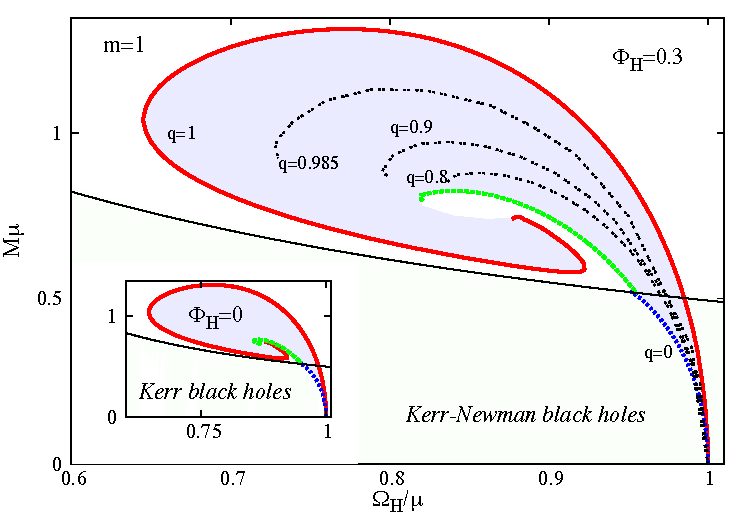
\includegraphics[width=0.48\textwidth]{papers/KerrNewman/BH-w-M} 
    \includegraphics[width=0.48\textwidth]{papers/KerrNewman/zoom-w-M}
  \end{center}
  \caption{The $(\Omega_H,M)$ domain of existence for a sample of KNBHsUSH. (Main left panel) Diagram for $\Phi_H=0.3$ with the boson star envelope (red solid line), the existence line on the domain of KN BHs (blue dotted line) and the line of extremal KNBHsUSH (green dashed line). The black solid line corresponds to the extremal KN BHs; non-extremal solutions exist below. The black dotted lines have constant normalized Noether charge $q$. (Inset) diagram for $\Phi_H=0$, for comparison. (Right panel) Detail around the intersection of the existence lines with the extremal KNBHsUSH lines and the extremal KN lines for $\Phi_H=0,0.6$ and $0.8$.  
	}
  \label{fig:w-M}
\end{figure}
%%%%%%%%%%%%%%%%%%%%%%%%%%%%%%%%%%%%%%%%%%%%%%%%%%%%%%%%%%%
 
  
 In Fig.~\ref{fig:w-g} (left panel), we exhibit the ratio $ M^{\Psi}/M$, which gives another measure of hairiness
   as a function of $\Omega_H$,
for $\Phi_H=0.3$. The figure shows that small fractions of the total energy in the hair are only allowed for sufficiently large horizon angular velocity. When the angular velocity is small, equilibrium between the hair and the horizon is only possible for solutions with $q$ close to unity, $i.e.$ boson star-like. 
The inset in this figure shows the $(\Omega_H,Q_E)$ domain of existence of the KNBHsUSH solutions. It illustrates that the electric charge of the solutions, for fixed $\Omega_H$ between that of the Hod point and the maximum allowed frequency, $\Omega_H=\mu$, is maximized along the existence line (and in particular at the Hod point). But for lower values of the frequency, slightly larger charges than that found at the Hod point are possible, occurring along the extremal hairy BHs line.

%%%%%%%%%%%%%%%%%%%%%%%%%%%%%%%%%%%%%%
\subsubsection{Gyromagnetic ratio}
%%%%%%%%%%%%%%%%%%%%%%%%%%%%%%%%%%%%%%
Rotating charges give rise to a magnetic dipole moment, $\mu_M$. 
In classical electromagnetism, a generic relation of the form~\eqref{gyro}, 
between $\mu_M$ and the total angular momentum, mass and charge can be derived, 
for systems with constant ratio of charge to mass density, yielding $g=1$. 
When experiments such as that performed for Stern and Gerlach in the early 20th century, 
showed that the electron should have $g=2$, it became clear that a new fundamental description 
for the electron was necessary, beyond the scope of the non-relativistic quantum theory. 
Such a description appeared with the Dirac equation, which, from first principles predicts $g=2$, 
a value that is corrected by loop diagrams in Quantum Electrodynamics (QED), 
yielding the so called anomalous magnetic moment, whose agreement 
with experiment is one of the outstanding successes of QED.

In BH physics, Carter first observed that $g=2$ for the KN solution. 
Since then many other studies considered the gyromagnetic ratio of rotating charged BHs, 
for instance with different asymptotics and in higher dimensions (see $e.g.$~
\cite{Garfinkle:1990ib,Herdeiro:2000ap,Aliev:2004ec,Ortaggio:2006ng,Aliev:2006tt}). 
Here we show that the addition of scalar hair leads to a suppression of the gyromagnetic ratio, 
and of the corresponding magnetic dipole moment, 
with respect to that of a comparable KN BH.  
 A novel aspect is that $g$ 
can be smaller than 1, a rather unsual feature in other models of relativistic, 
charged and spinning compact objects, 
$cf.$~\cite{Novak:2003uj}. 


In Fig.~\ref{fig:w-g} (right panel), we exhibit the gyromagnetic ratio in a $(q,g)$-diagram, for KNBHsUSH with $\Phi_H=0.3$.
The diagram shows that the gyromagnetic ratio, $g$, of both the extremal and non-extremal hairy BH solutions, is always less than $2$.
As expected, it does approach $2$, for both cases, in the limit of vanishing hair.
Further insight is obtained by considering the quantity
\begin{align}
\Delta\equiv \frac{M^2}{Q_E^2+J^2/M^2} \ ,
\end{align}
which determines the KN bound $\Delta\geqslant 1$. Indeed, all KN BHs have $\Delta>1$. This bound is, however, violated by a large set of KNBHsUSH, in particular by those close to the BS limit. This is reminiscent of what has been found for KBHsSH - see the discussions in~\cite{Herdeiro:2014goa,Herdeiro:2015gia,Herdeiro:2015tia,Delgado:2016zxv}.  Our results show that
solutions with $g<1$ predominantly exhibit $\Delta<1$ and thus violate the KN bound -- $cf.$ the inset of Fig.~\ref{fig:w-g} (right panel).



%%%%%%%%%%%%%%%%%%%%%%%%%%%%%%%%%%%%%%%%%%%%
\begin{figure}[H]
  \begin{center}
    \includegraphics[width=0.48\textwidth]{papers/KerrNewman/Mpsi}
    \includegraphics[width=0.48\textwidth]{papers/KerrNewman/qg}
  \end{center}
  \caption{(Left panel) The ratio $M^\Psi/M$ is shown as a function of $\Omega_H$ for a sample of KNBHsUSH. The inset shows the electric charge as a function of $\Omega_H$, where the blue dotted line is the existence line. 
	(Right panel)  The $(q,g)$ space. The inset show $g$ as a function of $\Delta$, that determines the KN bound.
}
\label{fig:w-g} 
\end{figure}
%%%%%%%%%%%%%%%%%%%%%%%%%%%%%%%%%%%%%%%%%%%%

 
 


%%%%%%%%%%%%%%%%%%%%%%%%%%%%%%%%%%%%%%%%%%%%
\section{Gauged scalar field model}
\label{sec_mod_g}
%%%%%%%%%%%%%%%%%%%%%%%%%%%%%%%%%%%%%%%%%%%%




%%%%%%%%%%%%%%%%%%%%%%%%%%%%%%%%
\subsection{Main differences in the model}

%%%%%%%%%%%%%%%%%%%%%%%%%%%%%%%%

Let us now consider the model described in Section~\ref{sec_mod_u} but with a \textit{gauged} scalar field, 
that couples minimally to the electromagnetic field, with gauge coupling $q_E$. 
This coupling is implemented by replacing the partial derivatives of the scalar field in the action~\eqref{KNaction} as
\begin{equation}
\partial_a \Psi \longrightarrow D_a\Psi=\partial_a \Psi + iq_E A_a \Psi \ .
\label{KNmc}
\end{equation}
The Einstein equations still take the form~\eqref{KNeom}, but with the substitution~\eqref{KNmc} 
in the scalar field energy-momentum tensor~\eqref{KNemt}. Then, the scalar and Maxwell equations of motion become
\begin{eqnarray}
\label{field-eqs}
D_{a}D^{a}\Psi=\mu^2 \Psi\ , \qquad 
\nabla_{b}F^{ba}=
iq_E \big [ (D^{a}\Psi^*) \Psi-\Psi^*(D^a \Psi) \big ] 
\equiv q_E j^a  \ .
\end{eqnarray}  
Physically, the scalar field is now electrically charged, 
and its quanta, the scalar particles, carry a charge $q_E$.
Thus the scalar field sources the Maxwell field.

This model is invariant under the $local$ U(1) gauge transformation 
\begin{eqnarray}
\label{gauge-transf}
\Psi \to \Psi e^{-i q_E \alpha}\ ,~~A_a\to A_a+\partial_a \alpha \ ,
\end{eqnarray}
where $\alpha$ is a real function. One consequence of this gauge invariance is that the $(t, \varphi)$-dependence of the scalar field ansatz~\eqref{eqn:field-ansatz}, 
can now be gauged away by applying the local $U(1)$ symmetry
(\ref{gauge-transf})
with $\alpha =  (m\varphi -w t)/q_E$.  This, however, also changes the gauge field, as $A_t\to A_t-w/q_E$,
$A_\varphi \to A_\varphi+m/q_E$. 
%
Consequently, the solutions cannot be constructed starting with the configurations in the
previous sections and increasing $q_E$.
%
Thus, in order
to be able to consider this approach, we  keep the $(t,\varphi)$-dependence in 
the scalar field ansatz and fix the corresponding gauge freedom by setting $A_t = A_\varphi = 0$ at infinity.

One major difference with respect to the case 
discussed in the previous section 
 is that the solitonic limit of the solutions carries now a nonzero electric charge.
Self-gravitating charged boson stars were first considered, in spherical symmetry, in~\cite{Jetzer:1989av} 
(see also the recent work  \cite{Pugliese:2013gsa}). 
To the best of our knowledge, no rotating generalizations of these static solutions have been reported\footnote{ 
Some properties of the spinning charged solitons, 
with a self-interacting ($Q$-ball type) scalar field model, were addressed in~\cite{Brihaye:2009dx}.
}.
The Noether charge $Q$ of the solitons, $i.e.$ the total
particle number, is now intrinsically related to the electric charge $Q_E$. 
The former can be computed as  
%
\begin{eqnarray}
\label{Q1}
Q= \int j^t \sqrt{-g} dr  d\theta d\varphi=
 4\pi \int_{0}^\infty dr \int_0^\pi d\theta  
~r^2\sin \theta ~e^{-F_0+2F_1+F_2}  (w-q_E A_t -mW)\phi^2 \ ,
\end{eqnarray}
%
whereas the latter is read from the asymptotics
 of the electric potential $A_t$, as given by Eq. \eqref{asym-matter-fields}.
A straightforward computation 
shows that both the Noether charge and the electric charge of the spinning \textit{solitons}
are proportional  to the total angular momentum,
\begin{eqnarray}
\label{JQ}
J= m Q=\frac{4 \pi m Q_E}{q_E}\ .
\end{eqnarray} 


%%%%%%%%%%%%%%%%%%%%%%%%%%%%%%%%%%%%%%%%%%%%%%%%%%%%%%%%%%%%%%%%%%
\subsection{Features of the gauged scalar field solutions}
\label{sec_results_g}
%%%%%%%%%%%%%%%%%%%%%%%%%%%%%%%%%%%%%%%%%%%%%%%%%%%%%%%%%%%%%%%%%%
 
The construction of the  gauged scalar field solutions is similar 
to that described above for the ungauged case ($q_E=0$ limit).
In particular, the KNBHsGSH are subject to the same set of 
boundary conditions  used in the ungauged case.
The synchronization condition, however, is different,   
\begin{equation}
\label{cond-new}
 w-q_E \Phi_H=m \Omega_H \ ,
\end{equation}
in agreement with the result found in the linear theory~\cite{Hod:2014baa,Benone:2014ssa}.

As mentioned in the introduction to this chapter, the electrically charged boson stars form a part of the domain of existence of KNBHsGSH. 
Thus we have paid special attention to this limiting case.
These solutions  are obtained by considering the ansatz~\eqref{eqn:HBH-ansatz}--\eqref{electric_ansatz} with $r_H=0$ 
and replacing the boundary conditions at the horizon,~\eqref{bch1} and \eqref{ABCs},
by the following boundary conditions at the origin
\begin{eqnarray}
\label{bc0} 
\partial_r F_i|_{r=0}= 
W|_{r=0}=0\ ,~~
\phi| _{r =0}=0\ ,~~\partial_r A_t|_{r=0}=A_\varphi|_{r=0}=0\ .
\end{eqnarray}
% 

Some results of the numerical integration are shown in Fig.~\ref{fig:w-M-gauged} (left panel).
The basic properties of the spinning gauged boson stars solutions can be summarized as follows.
First, for all values of the gauge coupling considered so far, 
the frequency dependence of the solutions is qualitatively similar to the ungauged case.
The solutions 
exist for a limited range of frequencies
$0<w_{min}<w<\mu$. 
In particular, we observe that the minimal frequency increases with $q_E$. 
After this minimal frequency, a backbending towards larger values of $w$ occurs, yielding a second branch of solutions. 
A second backbending, towards
smaller values of $w$,  is observed as the frequency reaches a maximal value along the second branch, $w\to w^{\rm 2nd}_{\rm max}$, whose value increases again with $q_E$. 
Then, similarly to the ungauged limit, a third branch of solutions develops -- not shown in Fig.~\ref{fig:w-M-gauged} (left panel).
Subsequently, we expect the existence of an inspiraling behaviour of the solutions, 
in analogy with uncharged boson stars, towards a limiting configuration.  


%%%%%%%%%%%%%%%%%%%%%%%%%%%%%%%%%%%%%%%%%%%%%%%%%%%%%%%%%%%
\begin{figure}[H]
  \begin{center}
    \includegraphics[width=0.48\textwidth]{papers/KerrNewman/BS-w-M-gauged}
    \includegraphics[width=0.48\textwidth]{papers/KerrNewman/BS-g-M-gauged}
  \end{center}
  \caption{
	(Left panel)
	The $(w,M)$ diagram for spinning boson stars with $q_E=0$ (red curve), $q_E/\mu=0.2, 0.3, 0.4, 0.5$
	and $0.6$ (top curve).  
		(Right panel)
	The mass $M$ is shown as a function of the gauge coupling constant $q_E$
	for several frequencies, $w/\mu=0.7, 0.8, 0.9$ and $0.95$ (as an inset).	}
  \label{fig:w-M-gauged}
\end{figure}
 %%%%%%%%%%%%%%%%%%%%%%%%%%%%%%%%%%%%%%%%%%%%%%%%%%%%%%%%%%%
Although only the mass is displayed in Fig.~\ref{fig:w-M-gauged} (left panel), the $J(w)$
diagram has a very similar shape.
Consequently,  the axially symmetric gauged boson stars do not possess
a static limit.  Observe also that the maximal mass of spinning gauged boson stars solutions increases with $q_E$.

As shown in Fig.~\ref{fig:w-M-gauged} (right panel), 
the solutions possess also a nontrivial dependence on 
the gauge coupling constant $q_E$.
For given values of $w$,
spinning solutions exist up to a maximal
value of the gauge coupling constant only, $q_E=(q_E)_{max}$.
The physical rationale behind this behaviour 
is similar to that discussed for the spherically symmetric case 
\cite{Jetzer:1989av,Pugliese:2013gsa}.
For $q_E>(q_E)_{max}$ the charge repulsion  becomes bigger than
  the scalar and gravitational attraction and localized solutions cease to exist  
(note that the maximal value of $q_E$
increases with frequency).
Also, as seen in Fig.~\ref{fig:w-M-gauged} (right panel),
all global charges stay finite as $q_E\to (q_E)_{max}$.

\bigskip

KNBHsGSH are obtained by adding a horizon at the center of the spinning gauged boson star  
we have just described, which can be done for  any such  solution.
One way to construct the BHs
  is to  start from  boson stars 
and slightly increase the horizon size via the parameter $r_H$.
In this approach, the other input parameters 
$\Omega_H$, $q_E$,  $\Phi_H$ and $m$
are kept fixed. 
We recall that for BHs, the frequency $w$ is fixed by the synchronization condition (\ref{cond-new}).
Then one finds three 
possible behaviours for
the resulting branches of BH solutions -- see Fig.~\ref{fig:q-AH-gauged} (left panel).
($i$) First, for small enough values of $\Omega_H$,
 the branch of BHs connects two different boson stars; 
as $r_H\to 0$ the horizon area vanishes, $q\to 1$, while the temperature
 diverges.
($ii$) For intermediate values of  $\Omega_H$,
the branch of solutions ends in an extremal KNBHsGSH solution. 
These limiting configurations have finite
horizon size   and global charges, $0<q<1$ and appear to possess 
a regular horizon.
($iii$) Finally, for large values of $\Omega_H$,
the branch of  KNBHsGSH interpolates between 
a charged boson star and a set of critical KN solutions (with $q=0$ and $A_H>0$), which lie again 
on an {\it existence line}. 

 In Fig.~\ref{fig:q-AH-gauged} (right panel) we exhibit the (Komar) energy density and angular momentum density (in the inset) for an illustrative example of a KNBHGSH  with physical input parameters 
$r_H=0.24$, $w =0.86$, $q_E =0.2$, $\Phi_H=0.1$. 
These densities have a contribution from both the electromagnetic and the scalar field. The main feature we wish to emphasize is the composite structure revealed by the plots. KN BHs have an (electromagnetic) energy and angular momentum density that decays with the radial coordinate, whereas KBHsSH 
(and boson stars)
have toroidal-like distributions for the (scalar) energy and angular momentum densities. 
Consequently, KNBHsGSH exhibit a superposition of these two behaviours, with decaying densities from the horizon but which exhibit a local maximum, in the neighbourhood of the equatorial plane, at some finite radial coordinate. 
A similar energy and angular momentum distribution can be found for KNBHsUSH.  

The behaviours illustrated in Fig.~\ref{fig:q-AH-gauged} supports the expectation that the domain of existence of KNBHsGSH will fill in the domain delimited by the boson star curves exhibited in Fig.~\ref{fig:w-M-gauged} (left panel), together with the existence line of KN BHs and a line of extremal KNBHsGSH,  in a qualitatively similar fashion to that shown in Fig.~\ref{fig:w-M} (left panel). Having established these solutions exist, and that their domain of existence will be analogue to the case of KNBHsUSH, we will not enter further details here.
Here we mention only that, similar to the ungauged case, 
the gyromagnetic ratio of  KNBHsGSH constructed so far is always smaller than $g=2$.


%%%%%%%%%%%%%%%%%%%%%%%%%%%%%%%%%%%%%%%%%%%%%%%%%%%%%%%%%%%
\begin{figure}[H]
  \begin{center}
    \includegraphics[width=0.48\textwidth]{papers/KerrNewman/BH-q-AH} 
    \includegraphics[width=0.48\textwidth]{papers/KerrNewman/energy-2d} 
  \end{center}
  \caption{ (Left panel) 
	The $(A_H,q)$ diagram is shown for three sets of KNBHsGSH solutions with fixed values of 
$\Omega_H$ and 
$q_E/\mu=0.2$, 
$\Phi_H=0.1$. (Right panel) 
 Energy density (and angular momentum density in the inset) along three different slices of constant $\theta$ for an illustrative example of a KNBHGSH.
	}
  \label{fig:q-AH-gauged}
\end{figure}
 %%%%%%%%%%%%%%%%%%%%%%%%%%%%%%%%%%%%%%%%%%%%%%%%%%%%%%%%%%%
 


%%%%%%%%%%%%%%%%%%%%%%
\section{Discussion}
\label{sec_remarks}
%%%%%%%%%%%%%%%%%%%%%%%

% The Kerr solution~\cite{Kerr:1963ud}, which describes the paradigmatic BH geometry in General Relativity, allows a generalization with electric (or magnetic) charge~\cite{Newman:1965my}, discovered shortly after the Kerr metric. Much more recently, it was found that the Kerr solution also allows a generalizations with scalar~\cite{Herdeiro:2014goa,Herdeiro:2015gia,Kleihaus:2015iea,Herdeiro:2015tia,Chodosh:2015oma} or Proca hair~\cite{Herdeiro:2016tmi}. The former are known as Kerr BHs with scalar hair (KBHsSH).
In this chapter we showed that electric charge can be added to KBHsSH, both considering an ungauged and a gauged scalar field and analysed some basic properties of the solutions.
In both cases, their domain of existence is qualitatively similar to the of the uncharged hairy BHs.
In particular it is bounded by three curves, corresponding do the solitonic limit (boson stars), extremal hairy BHs, and bald (KN) BHs.
In the gauged case, the solitonic limit corresponds to rotating charged boson stars, which until now had not been studied in the literature. 

These results indicate that by adding scalar hair to the electrically charged Kerr-Newman blackhole suppresses some of the electromagnetic properties of the black hole.
As an example of this we have considered the gyromagnetic ratio, $g$, and found that it is always lower than the well known the relativistic (Dirac) value for Kerr-Newman black holes, $g=2$~\cite{Carter:1968rr}, only reaching the limit when the hair vanishes.

There are other interesting applications for these solutions such as testing the no-short-hair conjecture.
This will be discussed further in Chapter \ref{ch:conclusions}.
\chapter{Conclusions}
\label{ch:conclusions}

\epigraph{``\emph{
Sól tr sortna, \\
sígur fold í mar, \\
hverfa af himni \\
heiðar stjörnur. \\
Geisar eimi \\
við aldurnara, \\
leikur hár hiti \\
við himin sjálfan. 
} 
''}{55th verse of Völuspá}


This thesis studied the phenomena of hairy black holes on the background of Kerr black holes.
Namely, we showed that Kerr black holes can support self-interacting scalar hair, Proca hair and that Kerr-Newman black holes can support both gauged and ungauged scalar hair.

To this end, we first discussed $Q$-clouds in Chapter \ref{ch:Q}.
$Q$-clouds are rotating generalizations of the well known flat space $Q$-balls and are in synchronous rotation with the black hole horizon.
When compared to their scalar cloud counterparts, we found that the subset of Kerr black holes which can support scalar clouds expands from a one-dimensional line to a two-dimensional subspace of Kerr black holes in the case of $Q$-clouds.
In Chapter \ref{ch:SI}, we added positive $\phi^4$-self-interactions to Kerr black holes with scalar hair and found that, just as for their self-interacting boson star counterparts, their mass increases.
However, this mass increase arises solely from the scalar field and not the horizon.
As such, we have called these solutions ``hairier but not heavier''.
At the end of this chapter, we showed that by allowing the $Q$-clouds of the previous chapter to backreact on the spacetime, hairy black hole solutions are found.
We found that these self-interacting KBHsSH, with now a different self-interaction potential, are also ``hairier but not heavier''.

\bigskip

In Chapter \ref{ch:proca}, we exchanged the scalar field for a massive vector field, i.e. a Proca field.
We found Kerr black holes with Proca hair and these solutions have a similar structure as their scalar hair counterparts yet their energy densities possess a second local maximum which could provide interesting phenomenology.
This seems to indicate that these objects, as well as their soliton counterparts are ``composite objects''.
A consequence of this is a negative region of the angular momentum density which leads to a counter-rotating toroidal-like region in the spacetime.
The existence of KBHsPH -- to the best of our knowledge the first example of (fully non-linear)   
BHs with (Abelian) vector hair -- is anchored  in the synchronization/superradiance condition
%
All previously constructed examples which employed this mechanism have scalar hair, 
both in four spacetime dimensions~\cite{Herdeiro:2014goa,Herdeiro:2015gia,Kleihaus:2015iea,Herdeiro:2015tia} and in higher dimensions~\cite{Brihaye:2014nba,Herdeiro:2015kha}, 
including the example in five dimensional asymptotically Anti-de-Sitter space found in~\cite{Dias:2011at}. 

Several direct generalizations/applications of these solutions are possible. 
At the level of constructing further 
solutions, we anticipate that 
$(i)$ self-interacting Proca hair will lead to new solutions, 
which, if the scalar field case is a good guide, can have a much larger ADM mass (but not horizon mass) as we saw in Chapter \ref{ch:SI} for solutions with scalar hair,
and
$(ii)$ hybrid solutions with scalar \emph{and} Proca hair are possible. 
At the level of possible astrophysics phenomenology, 
it would be interesting to look in detail to the geodesic flow, 
in particular to the frequency at the innermost stable circular orbit (ISCO), 
quadrupoles as well as to the lensing and shadows of these new black holes and stars,
following~\cite{Cunha:2015yba} (see also the review~\cite{Johannsen:2015mdd}). 

\bigskip

Finally, in Chapter \ref{ch:KN}, we studied both gauged and ungauged scalar hair around Kerr-Newman black holes.
We found that while these solutions are very similar to their uncharged counterparts they do possess some interesting features.
E.g. some electromagnetic properties, such as the gyromagnetic ratio, seem to be suppressed in the presence of scalar hair.
The gyromagnetic ratio measures how a magnetic dipole moment is induced by the charge and angular momentum of the BH.
It is well known that the relativistic value holds for the Kerr-Newman BH, i.e. $g=2$~\cite{Carter:1968rr}.
We have shown that the gyromagnetic ratio of these hairy charged BHs is always $g\leqslant 2$, with equality attained only in the ``bald'' case.
Thus, the scalar hair leads to a suppression of the magnetic dipole moment.
This property is also present in the case of charged rotating boson stars.

As an example of other interesting applications for these solutions we mention testing the no-short hair conjecture.
This conjecture suggests that when hair exists around a spherically symmetric black hole, it should extend beyond $3r_+/2$, where $r_+$ is the areal radius of the event horizon\cite{Nunez:1996xv}.
This radius is in fact the location of the circular null geodesic for the Schwarzschild solution, which leads to a general version of the conjecture that the hair must extend beyond the null circular orbit of the spacetime\cite{Hod:2011aa}.
For linearized hair around rotating black holes, the conjecture seems to hold for uncharged black holes\cite{Hod:2016dkn}, but may be violated for electrically charged ones~\cite{Hod:2014sha,Hod:2015ynd}.
The latter possibility can be tested using the fully non-linear solutions of the Einstein-Maxwell-Klein-Gordon field equations discussed in Chapter \ref{ch:KN}.

Future work could also include the phenomenological studies discussed for the Proca model above, but now for these electrically charged solutions.
Due to the more complicated spatial distributions of energy densities and other quantities, one would expect some qualitative differences.

\bigskip

The connection between KBHsSH and superradiance led to the suggestion that, underlying the example of KBHsSH, there is a more general mechanism~\cite{Herdeiro:2014goa,Herdeiro:2014ima} (see also~\cite{Herdeiro:2015waa,Herdeiro:2015gia}) at play.
In Chapter \ref{ch:proca} we formally put forth the conjecture and confirmed it for a handful of configurations throughout this thesis.
Essentially it seems that any rotating black hole can be endowed with synchronized bosonic hair.
Generalizations to spin $2$ fields should be straight forward though it is not clear which equations of motion should be used.

However, in higher dimensions it was shown that superradiance is not a required ingredient for these hairy black hole solutions to exist \cite{Brihaye:2014nba,Herdeiro:2015kha}.
This seems to indicate that while superradiance hints of their existence, it is really the synchronization condition that plays a key role in the existence of such solutions.

\chapter{Outlook}
\label{ch:outlook}

\epigraph{``\emph{
Sér hún upp koma \\
öðru sinni \\
jörð úr ægi \\
iðjagræna. \\
Falla fossar, \\
flýgur örn yfir, \\
sá er á fjalli \\
fiska veiðir. 
} 
''}{57th verse of Völuspá}

Let us now briefly discuss the outlook of this new field of hairy black holes.
If we look towards more astrophysical horizons, these new black hole solutions have interesting phenomenology.
As was discussed in \cite{Herdeiro:2014goa,Herdeiro:2015gia}, the frequency at the ISCO and the quadrupole moment changes for these types of hairy black hole solutions.
The results in Chapter \ref{ch:SI} indicate that large differences might occur when considering these properties in terms of ADM quantities but not in terms of horizon quantities.

Another pursuit lies in the shadows and gravitational lensing of these black holes \cite{Cunha:2015yba,Cunha:2016bjh} and their corresponding ``star solutions''.
In Fig. \ref{shadows}, we show a striking example of the shadows of a KBHsSH and the Kerr black hole whose mass and angular momenta are that of the ADM mass and angular momenta of the KBHsSH.
Though this is just one example, it is clear even by the naked eye that there is a difference in both the shape and size of the shadow.

\begin{figure}[h!]
\centering
  \includegraphics[width=0.48\textwidth]{Figs/skuggi2a.pdf}
  \includegraphics[width=0.48\textwidth]{Figs/skuggi2b.pdf}
  \caption{(Left) The shadow of a KBHsSH with parameters $M_{\rm ADM}=0.933$, $J_{\rm ADM}=0.74$, $M_H=0.234$ and $J_H=0.115$. (Right) The shadow of a Kerr black hole with the same ADM parameters as the KBHsSH on the left.}
\label{shadows}
\end{figure}

The shadows of the three new cases of Kerr black holes with hair in this thesis could provide more templates for the shape of a black hole shadow.
Even though some of them might not be of much astrophysical interest, they still provide alternative, and important, templates for future observations.

\bigskip

The physical and phenomenological consequencies of these new types of hairy black holes are still in its infancy.
A particularly important question concerns the stability of these new solutions, which must be studied further.

The charged counterpart to superradiance discussed in the introduction, i.e. a gauged scalar field on the background of a Reissner-Nordström black hole, has been shown to form dynamically \cite{Sanchis-Gual:2015lje}.
This, as the charged case is often considered a toy model for the more technically difficult rotating example, provides some hints that the hairy black holes studied in this thesis are really the endpoint of the superradiant instability for each corresponding configuration of field and black hole.

In~\cite{Herdeiro:2014jaa} it was suggested that Kerr black holes with hair may be afflicted by superradiant instabilities, as they possess an ergoregion which is a crucial ingredient of the superradiant instability of the Kerr black hole.
But it was also argued that these superradiant instabilities may be ``weaker''  than for Kerr.
I.e. that the timescale might be longer.
Note however that even if they are unstable in this way, they could still play a role in astrophysical processes if the timescale of the instability is long enough.
As an example consider the merger of two hairy black holes: if the merger timescale is smaller than that of the instability, the hair will play a role nonetheless.
Therefore, even though we suspect these black holes to be unstable towards various types of instabilities, the question still remains whether they could play an important role in astrophysical processes.
The full time evolution, both for a single black hole or a pair of them, will therefore give important insights into the true nature of these solutions.

% math paper \cite{Chodosh:2015oma}. include it or not?

\bigskip

Finally, it is still very common to find in the current literature of black holes statements that stationary black holes in General Relativity are described solely by mass, angular momentum and charge.
As was shown in this thesis, and the work it is based on, this is \textit{not true as a generic statement for General Relativity, even if physical matter -- i.e. obeying all energy conditions -- is required.}
These examples show that Noether charges, rather than charges associated to Gauss laws, are also permitted in non-pathological stationary, asymptotically flat, black hole solutions. 
The question is then whether these Noether charges can survive in real dynamical processes.

\bigskip

To end this thesis, I quote Chandrasekhar once again

\begin{quote}
    \emph{``In my entire scientific life...the most shattering experience has been the realization that an exact solution of general relativity, discovered by the New Zealand mathematician Roy Kerr, provides the absolutely exact representation of untold numbers of massive black holes that populate the Universe.''}
\end{quote}

and conclude that things may not be as simple as they seem.

